%\begin{filecontents}
%  @CONTROL{apsrev41Control,title="0"%,author="48",editor="1",pages="1",year="0"}
%\end{filecontents}
\RequirePackage[l2tabu, orthodox]{nag}
\RequirePackage{fixltx2e}
\RequirePackage{fix-cm}
\PassOptionsToPackage{pdftex,psdextra=true,
pdfversion=1.7,
pdfencoding=auto,
pdfnewwindow=true,
pdfusetitle=true,
psdextra=true,
%pdftoolbar=true,
%pdfmenubar=true,
bookmarks=true,
bookmarksnumbered=true,
bookmarksopen=true,
pdfpagemode=UseThumbs,
bookmarksopenlevel=1,
pdfpagelabels=false
}{hyperref}
\PassOptionsToPackage{usenames,dvipsnames}{xcolor}
\documentclass[aps,english,superscriptaddress,onecolumn,twoside,longbibliography,pra,floatfix,fleqn,nofootinbib]{revtex4-1}%


\usepackage[utf8]{inputenx}% for arXiv use encoding ansinew
\input{ix-utf8enc.dfu}
%\usepackage[utf8x]{inputenc}% for arXiv use encoding ansinew
%\usepackage{utf8mathlite}% custom style sheet for unicode-ish math
%\usepackage{newunicodechar}
%\newunicodechar{∫}{\int}
%\usepackage{unicode-math}
\usepackage[OT1]{fontenc}
\usepackage{ucs} %for unichar

\usepackage{amsfonts}
\usepackage{amssymb}
\usepackage{amsthm}
\usepackage[intlimits,fleqn]{amsmath}
%\usepackage{mathdots}
\usepackage{graphicx}%
\usepackage{placeins} %for FloatBarrier
\usepackage{afterpage} %for FloatBarrier in afterpage wrapper
%\usepackage{flushend}
%\usepackage{dblfloatfix}
\usepackage[normalem]{ulem} %for sout
\usepackage[raggedright,bf,nooneline]{subfigure}
\renewcommand{\thesubfigure}{\alph{subfigure}}
\usepackage{paralist}

%\usepackage{ellipsis}
\usepackage{float}% (not with floatrow)
\usepackage{wrapfig}
%\usepackage{floatrow}


\usepackage{setspace}
\usepackage{array}
\usepackage{ragged2e}%for justifying text in tables
\usepackage{tabularx}
\def\tabularxcolumn#1{m{#1}}
\usepackage{booktabs}
%\usepackage{tabulary}
\newcolumntype{R}{>{\raggedleft\arraybackslash}X}
\newcolumntype{C}{>{\centering\arraybackslash}X}
\newcolumntype{L}{>{\raggedright\arraybackslash}X}
\newcolumntype{J}{>{\justifying\arraybackslash}X}
\usepackage{adjustbox}
\usepackage{multirow}
\newcolumntype{T}[2]{%
    >{\adjustbox{angle=#1,lap=\width-(#2)}\bgroup}%
    l%
    <{\egroup}%
}
\newcommand*\rot{\multicolumn{1}{T{90}{1em}}}% no optional argument here, please!

\setcounter{MaxMatrixCols}{30}
\providecommand{\U}[1]{\protect\rule{.1in}{.1in}}
%EndMSIPreambleData
\newtheorem{theorem}{Theorem}
\newtheorem{acknowledgement}[theorem]{Acknowledgement}
\newtheorem{algorithm}[theorem]{Algorithm}
\newtheorem{axiom}[theorem]{Axiom}
\newtheorem{claim}[theorem]{Claim}
\newtheorem{conclusion}[theorem]{Conclusion}
\newtheorem{condition}[theorem]{Condition}
\newtheorem{conjecture}[theorem]{Conjecture}
%\newtheorem{corollary}[theorem]{Corollary}
\newtheorem{corollary}{Corollary}[theorem]
\newtheorem{criterion}[theorem]{Criterion}
\newtheorem{definition}[theorem]{Definition}
%\newtheorem{example}[theorem]{Example}
\newtheorem{exercise}[theorem]{Exercise}
\newtheorem{lemma}[theorem]{Lemma}
\newtheorem{notation}[theorem]{Notation}
\newtheorem{problem}[theorem]{Problem}
\newtheorem{prop}{Proposition}
\newtheorem{taut}{Tautology}
\newtheorem{remark}[theorem]{Remark}
\newtheorem{solution}[theorem]{Solution}
\newtheorem{summary}[theorem]{Summary}
%\newenvironment{proof}[1][Proof]{\noindent\textbf{#1.} }{\ \rule{0.5em}{0.5em}}

% hyperlink stuff
\usepackage[usenames,dvipsnames]{xcolor}
\definecolor{ultramarine}{RGB}{63, 0, 255}
\definecolor{medblue}{RGB}{0, 0, 100}
\definecolor{panblue}{RGB}{0,24,150}
\definecolor{carmine}{RGB}{150, 0, 24}
\usepackage[breaklinks=true]{hyperref}
\hypersetup{colorlinks,
linkcolor=carmine,
citecolor=medblue,
urlcolor=panblue,
anchorcolor=OliveGreen}
%\usepackage{url}
\usepackage{pdfpages}

\definecolor{purple}{RGB}{128,0,128}
\definecolor{PURPLE}{RGB}{128,0,128}
\definecolor{BLACK}{RGB}{0,0,0}
\definecolor{ultramarine}{RGB}{63, 0, 255}
\definecolor{medblue}{RGB}{0, 0, 100}
\definecolor{panblue}{RGB}{0,24,150}
\definecolor{carmine}{RGB}{150, 0, 24}
\definecolor{gray}{RGB}{150, 150, 150}

\newcommand{\purp}[1]{{\color{purple}{#1}\color{black}}}
\newcommand*{\mred}[1]{{\color{RawSienna}{\mathbf{#1}}}}
\newcommand*{\mblue}[1]{{\color{MidnightBlue}{\ensuremath{#1}}}}
\newcommand*{\mpurp}[1]{{\color{Plum}{\mathbf{#1}}}}
\newcommand*{\mgreen}[1]{{\color{OliveGreen}{\mathbf{#1}}}}
\newcommand*{\tred}[1]{{\color{carmine}{\textbf{#1}}}}
\newcommand*{\tblue}[1]{{\color{MidnightBlue}{\textbf{#1}}}}
\newcommand*{\tpurp}[1]{{\color{Plum}{\textbf{#1}}}}
\newcommand*{\tgreen}[1]{{\color{Sepia}{\textbf{#1}}}}

\newcommand{\quoteby}{\raise.17ex\hbox{$\scriptstyle\sim$}}

\usepackage{verbatim} %for comment command
\usepackage{units}% for nicefrac
\newcommand{\half}[1]{\nicefrac{#1}{2}}

%\usepackage{braket} %provide \bra and \Bra and \set and \Set etc...
%\newcommand{\brackets}[1]{\lbrace{#1\rbrace}}
%\newcommand{\brackets}{\Set}



\usepackage{microtype}
%\usepackage{MnSymbol}
%\usepackage{mathabx}

\usepackage[capitalise]{cleveref}
\Crefname{eqs}{Eqs.}{Eqs.}

\creflabelformat{eqs}{(#2#1#3)}
\crefrangelabelformat{equation}{(#3#1#4-#5#2#6)}
%\crefmultiformat{equation}{eqs.~(#2#1#3)}{ and~(#2#1#3)}{, (#2#1#3)}{ and~(#2#1#3)}
\Crefmultiformat{equation}{Eqs.~(#2#1#3}{,#2#1#3)}{,#2#1#3}{,#2#1#3)}
\crefrangelabelformat{eqs}{(#3#1#4-#5#2#6)}
\Crefmultiformat{eqs}{Eqs.~(#2#1#3}{,#2#1#3)}{,#2#1#3}{,#2#1#3)}
\Crefname{prop}{\textbf{Prop}.}{\textbf{Props}.}
\Crefname{taut}{\textbf{Taut}.}{\textbf{Tauts}.}
\Crefname{section}{Sec.}{Secs.}

%\Crefname{ineq}{Ineq.}{Ineqs.}
%\creflabelformat{ineq}{(#2#1#3)}
%\crefrangelabelformat{ineq}{(#3#1#4-#5#2#6)}
%\Crefmultiformat{ineq}{Ineqs.~(#2#1#3}{,#2#1#3)}{,#2#1#3}{,#2#1#3)}

%\Crefname{ineqs}{Ineqs.}{Ineqs.}
%\creflabelformat{ineqs}{(#2#1#3)}
%\crefrangelabelformat{ineqs}{(#3#1#4-#5#2#6)}
%\Crefmultiformat{ineqs}{Ineqs.~(#2#1#3}{,#2#1#3)}{,#2#1#3}{,#2#1#3)}

\newenvironment{topic}[1][]{\par\medskip\noindent\textbf{\rmfamily#1}}{\par\medskip\par}

\newcounter{step}[section]
\newenvironment{step}[1][]{\refstepcounter{step}\par\medskip
   \noindent \textbf{Step~\thestep}\rmfamily#1}{\par\medskip\par}
%\newenvironment{step}[1][Step]{\noindent\textbf{#1.} }{\ \rule{0.5em}{0.5em}}
\Crefname{step}{Step}{Steps}
\creflabelformat{step}{#2#1#3}
\crefrangelabelformat{step}{#3#1#4-#5#2#6}
\Crefmultiformat{step}{Steps.~#2#1#3}{,#2#1#3}{,#2#1#3}{,#2#1#3}
\renewcommand{\thestep}{\arabic{step}}


\newcounter{example}[section]
\newenvironment{example}[1][]{\refstepcounter{example}\par\medskip
   \noindent \textbf{Example~\theexample}\rmfamily#1}{\par\medskip\par}
%\newenvironment{step}[1][Step]{\noindent\textbf{#1.} }{\ \rule{0.5em}{0.5em}}
\Crefname{example}{Exmpl.}{Exmpls.}
\creflabelformat{example}{#2#1#3}
\crefrangelabelformat{example}{#3#1#4-#5#2#6}
\Crefmultiformat{example}{Exmpls.~#2#1#3}{,#2#1#3}{,#2#1#3}{,#2#1#3}
\renewcommand{\theexample}{\arabic{example}}


\usepackage[intlimits,fleqn]{mathtools} %for mathclap and prescript and more. Learning to love this package. And DeclarePairDelimeter!
\DeclarePairedDelimiter{\ceil}{\lceil}{\rceil}
\DeclarePairedDelimiter{\floor}{\lfloor}{\rfloor}
\DeclarePairedDelimiter{\parens}{\lparen}{\rparen}
\DeclarePairedDelimiter{\parenths}{\lparen}{\rparen}
\DeclarePairedDelimiter{\abs}{\lvert}{\rvert}
\DeclarePairedDelimiter{\norm}{\lVert}{\rVert}
\DeclarePairedDelimiter{\braces}{\lbrace}{\rbrace}
\DeclarePairedDelimiter{\bracks}{\lbrack}{\rbrack}
\DeclarePairedDelimiter{\expec}{\langle}{\rangle}
\newcommand{\brackets}[1]{\braces*{#1}}

%\usepackage{nath} %automatically pair delimiters. Provides \inline and \displayed. Adjusts \frac and /

%\newcommand{\na}{\ensuremath{\mathring{a}}}
%\newcommand{\nb}{\ensuremath{\mathring{b}}}
%\newcommand{\nc}{\ensuremath{\mathring{c}}}
\newcommand{\na}{\ensuremath{\overline{a}}}
\newcommand{\nb}{\ensuremath{\overline{b}}}
\newcommand{\nc}{\ensuremath{\overline{c}}}

\newcommand{\naf}{\ensuremath{\lnot a}}
\newcommand{\nbf}{\ensuremath{\lnot b}}
\newcommand{\ncf}{\ensuremath{\lnot c}}

\newcommand{\n}[1]{\ensuremath{\overline{#1}}}
\newcommand{\ot}[1]{\ensuremath{\overline{#1}}}
\newcommand{\Nor}[1]{\operatorname{\mathsf{Nor}}\!\bracks*{#1}}

\newcommand{\larray}[1]{\ensuremath{\begin{array}{l}#1\end{array}}}
\newcommand{\lparens}[1]{\ensuremath{\parens*{\larray{#1}}}}
%\newcommand{\NamedFunction}[2]{\operatorname{\mathsf{#1}}\!\bracks*{#2}}
%\newcommand{\NamedFunction}[2]{\operatorname{\mathsf{#1}}\!\bracks*{\larray{#2}}}
\newcommand{\NamedFunction}[2]{\operatorname{\mathsf{#1}}\!\begin{bmatrix*}[l]#2\end{bmatrix*}}
%\newcommand{\SmallNamedFunction}[2]{\operatorname{\mathsf{#1}}\bracks{#2}}
\newcommand{\SmallNamedFunction}[3][]{{\operatorname{\mathsf{#2}}_{#1}}\bracks{#3}}
\newcommand{\nap}{\ensuremath{a'}}
\newcommand{\nbp}{\ensuremath{b'}}
\newcommand{\ncp}{\ensuremath{c'}}
\newcommand{\napp}{\ensuremath{a''}}
\newcommand{\nbpp}{\ensuremath{b''}}
\newcommand{\ncpp}{\ensuremath{c''}}

\newcommand{\p}[2][]{{p_{#1}}\parenths{#2}}
%\newcommand{\pdf}[1]{\operatorname{\mathsf{PDF}}\!\parenths{#1}}
\newcommand{\pdf}[2][]{{P_{#1}}\parenths{#2}}
\newcommand{\pdfp}[2][]{{P_{#1}}^{\prime}\parenths{#2}}
\newcommand{\pfunc}[1]{P_{#1}}
\newcommand{\An}[2][]{{\mathsf{An}_{#1}}\parenths{#2}}
\newcommand{\Pa}[2][]{{\mathsf{Pa}_{#1}}\parenths{#2}}
\newcommand{\Ch}[2][]{{\mathsf{Ch}_{#1}}\parenths{#2}}
\newcommand{\subgraph}[2][]{{\operatorname{\mathsf{SubDAG}}_{#1}}\bracks{#2}}
\newcommand{\ansubgraph}[2][]{{\operatorname{\mathsf{AnSubDAG}}_{#1}}\bracks{#2}}
\newcommand{\pasubgraph}[2][]{{\operatorname{\mathsf{PaSubDAG}}_{#1}}\bracks{#2}}
\newcommand{\nodes}[1]{\SmallNamedFunction{Nodes}{#1}}
\newcommand{\edges}[1]{\SmallNamedFunction{Edges}{#1}}
\newcommand{\namedand}[1]{\SmallNamedFunction{And}{#1}}
\newcommand{\namedor}[1]{\SmallNamedFunction{Or}{#1}}
\newcommand{\aindep}{\ensuremath{\mathrel{\mathopen{\Lsh}{\scriptstyle\emptyset}\mathclose{\Rsh}}}}


%\newcommand{\subsim}[1]{\substack{\textstyle #1\\[-0.3ex]\sim}}
%\newcommand{\subsim}{\utilde}
%\def\subsim#1{\mathord{\vtop{\ialign{##\crcr
%$\hfil\displaystyle{#1}\hfil$\crcr\noalign{\kern1.5pt\nointerlineskip}
%$\hfil\tilde{}\hfil$\crcr\noalign{\kern1.5pt}}}}}
\newcommand{\subsim}[1]{\tilde{#1}}

\newcommand{\cramp}[1]{\ensuremath{\mathord{#1}}}
%\newcommand{\cramp}[1]{\ensuremath{\mathopen{}#1\mathclose{}}} oldway. New way is better.
\newcommand{\eql}{\cramp{=}}

\usepackage{bm}
\newcommand{\setlambda}{\bm{\lambda}}


%%%% Tobias: to mark my edits and stuff
\usepackage{showkeys}
\usepackage[draft]{fixme}
\newcommand{\btob}{\color{OliveGreen}}
\newcommand{\etob}{\color{black}}



\let\stdsection\section
%\renewcommand\section{\clearpage\stdsection}%every section new page


\begin{document}
%\preprint{ }
%\title{Transitivity of implication and causal structure}
\title{The Inflation DAG Technique for Causal Inference with Hidden Variables}
\author{Elie Wolfe}
\email{ewolfe@perimeterinstitute.ca}
\affiliation{Perimeter Institute for Theoretical Physics, Waterloo, Ontario, Canada, N2L 2Y5}
\author{Robert W. Spekkens}
\email{rspekkens@perimeterinstitute.ca}
\affiliation{Perimeter Institute for Theoretical Physics, Waterloo, Ontario, Canada, N2L 2Y5}
\author{Tobias Fritz}
\email{tobias.fritz@mis.mpg.de}
\affiliation{Perimeter Institute for Theoretical Physics, Waterloo, Ontario, Canada, N2L 2Y5}
\affiliation{Max Planck Institute for Mathematics in the Sciences, Leipzig, Germany}
\date{\today}


\begin{abstract}
\sout{The fundamental problem of causal inference is to infer from a given probability distribution over observed variables, what causal structures, possibly incorporating hidden variables, could have given rise to that distribution.}


The fundamental problem of causal inference is to infer if an observed probability distribution is compatible with some causal structure hypothesis, possibly incorporating hidden variables.
Given a particular causal structure, it is therefore valuable to derive incompatibility witnesses, i.e. criteria whose violation certifies the incompatibility of the violating distribution with the given causal structure.
The problem of causal inference via incompatibility witnesses comes up in many fields. Special incompatibility witnesses are Bell inequalities (which distinguish non-classical from classical distributions) and Tsirelson inequalities (which distinguish quantum from post-quantum distributions), and Pearl's instrumental inequality. All of these are limited to very specific causal structures. Analogues of such inequalities for more-general causal structures, i.e., necessary criteria for either classical or quantum distributions to be realizable from the structure, are highly sought after. 

We here introduce a technique for deriving such incompatibility witnesses, applicable to any causal structure. It consists of first \textit{inflating} the causal structure and then translating weak constraints on the inflated structure into stronger constraints on the original structure. Moreover, we show how our technique can be tuned to yield either classical criteria (i.e., that may have quantum violations), or post-classical criteria (i.e., that hold even in the context of general probability theories), depending on whether or not the inflation implicitly broadcasts the value of a hidden variable. Concretely, we derive polynomial inequalities for the so-called Triangle scenario, and we show how all Bell inequalities also follow from our method. %analyze Pearl's instrumental inequality from our perspective. 
Furthermore, given both a causal structure and a specific probability distribution, our technique can be used to efficiently witness their incompatibility, without requiring explicit inequalities. The inflation technique is therefore both relevant and practical for general causal inference tasks with hidden variables.

%We introduce a technique for deriving such inequalities which apply to any causal structure (with hidden variables). This class contains all Bell inequalities as special cases. Our technique consists of ``inflating'' the causal structure. We then translate weak constraints on the inflated structure into much stronger constraints on the original structure through ``deflation" and quantifier elimination. One can derive either classical causal infeasibility criteria (i.e. that have quantum violations), or criteria which hold even in the context of general probability theories, depending on whether the inflation relies on cloning the values of the hidden variables. Concretely, we derive polynomial inequalities for the so-called Triangle scenario, and we show how the well-known Bell inequalities also follow from our method.%analyze Pearl's instrumental inequality from our perspective. 
%Furthermore, our method can efficiently witness the incompatibility of a probability distribution with a given causal structure even absent explicit quantifier-free inequalities.

\end{abstract}
\maketitle
%In Ref.~\cite{WoodSpekkens}, the standard proof of Bell's theorem is presented in the language of causal inference.  In particular, the CHSH inequality emerges as a special case of what Pearl calls an ``instrumental inequality''.  Hardy's proof of Bell's theorem is quite different from the standard proof and the following question naturally arises: is there a generic tool for classical causal inference of which the Hardy argument can be considered a special case when applied to the M-shaped causal structure of the Bell experiment?

%To try and answer this question, we apply Hardy-type reasoning to the triangle causal structure, that is, the one with three observed variables, each pair of which have a common cause.  We show that this sort of reasoning does indeed facilitate causal inference in the case of the triangle causal structure, thereby lending some evidence to the notion that this style of argument has the potential to be generalized into a generic tool for classical causal inference.

\section{Introduction}

Given a probability distribution over some random variables, the problem of \tblue{causal inference} is to determine what causal relations among these variables and possibly also some unobserved variables could have generated this distribution. This type of problem arises in a wide variety of scientific disciplines, from sussing out biological pathways to enabling machine learning \cite{pearl2009causality,spirtes2011causation,studeny2005probabilistic,koller2009probabilistic}. A related problem is to determine, for a given set of causal relations, the set of all probability distributions that can be generated from them.   
%Progress on the latter problem can be leveraged towards solving the former problem because one can simply test a set of possible causal hypotheses for compatibility with a given distribution.  
%We focus here on the following decision problem:
%Both of these problems can be reduced in principle to the following decision problem: 
A special case of both is the following decision problem: given a probability distribution and a causal hypothesis, 
%start with \emph{both} a given distribution and a given causal hypothesis and\
 determine whether the two are compatible, in the sense that the causal relations permitted by the hypothesis could in principle have generated the given distribution. 
%For instance, in causal inference, one could in principle parametrize the set of possibilities for the causal relations and check each for compatibility with the given distribution, while in a sampling problem, one could in principle parameterize the set of probability distributions and check each for compatibility with the given causal hypothesis.  Of course, this reduction may not be computationally feasible in practice.  
%Nonetheless, the problem of deciding compatibility 
%This problem is already difficult enough on its own; it is the one we focus on in this article. 
%interesting in its own right.  It is the probem on which we will focus in this article. 
In this article, we focus on techniques for solving the decision problem and for finding necessary conditions on a probability distribution for compatibility with a given causal hypothesis.

%\tblue{infeasibility criteria}, i.e., observable constraints such that the their violation implies the invalidity of the hypothesis as an explanation for observational data. 

In the simplest setting, the causal hypothesis consists of a directed acyclic graph (DAG) whose nodes all correspond to {\em observed} variables.
%which only contains the observed variables as nodes. 
In this case, obtaining a verdict on the compatibility of a given distribution with the causal hypothesis is simple: the compatibility holds if and only if the distribution is Markov with respect to the DAG, which is to say that all of the conditional independence relations in the distribution are explained by the structure of the DAG. The compatible DAGs can be determined algorithmically solely from the distribution. \sout{ i.e.~without having an \emph{a priori} hypothesis}~\cite{pearl2009causality}.

A significantly more difficult case is when one considers a causal hypothesis which consists of a DAG whose nodes include \tblue{latent} variables, so that the set of observable variables is only a subset of the nodes of the DAG. This case occurs, e.g.,~in situations where one needs to deal with the possible presence of unobserved confounders, as in experiment design. \purp{What is ``experiment design''? Is this a technical term in statistics?  --RWS}

It is useful to distinguish two varieties of this problem. In the first case, the causal hypothesis specifies the nature of the latent variables, for instance, that they are discrete and of a particular cardinality (the cardinality of a variable is the number of possible values it can take).   In the second case, the nature of the latent variables is arbitrary.  

Consider the first case.  If the latent variables are all discrete then the mathematical problem which one must solve to infer the distributions that are compatible with the hypothesis is a quantifier elimination problem for some finite number of quantifiers.  The probability distribution over the observed variables are defined as a function of the conditional probabilities incorporating the latent variables, where this function is dictated by the DAG.  If one can eliminate the parameters describing these conditional probabilities, while taking into account the constraint that probabilities are constrained to the unit interval,  one is left with constraints that refer exclusively to the probability distribution over the observed variables.  Because this is a nonlinear quantifier elimination problem, it is infeasible to provide an exact solution except in very simple cases [cite:LeeSpekkens].  Nonetheless, because the mathematical problem to be solved is known in this case, any techniques developed for finding approximate solutions to problems of nonlinear quantifier elimination can be leveraged.

The second case, where the latent variables are arbitrary, is more difficult, but also the case that has been the focus of most research and that motivates the present work.  
%While the conditional independence relations implied by the causal structure on the observable nodes are still necessary conditions for compatibility of a distribution with the causal structure hypothesis, these equations are generally no longer sufficient.  
It is possible that it is also reducible to 
%It is not obvious, a priori, whether or not this case can be formulated as 
a quantifier elimination problem for quantifiers that refer to the latent variables. This would be the case, for instance, if one could show that discrete latent variables of a certain finite cardinality (rather than arbitrary latent variables) are sufficient to generate all the distributions compatible with that DAG (see, e.g.~\cite{} [cite unpublished Rosset result]).   However, it is not clear at present whether this is likely to be the case, and we do not pursue the question here.  At present, therefore, the problem of providing a mathematical algorithm for deciding compatibility in this second case---let alone an efficient algorithm---remains open.
%In any case, it is not the approach we pursue here. 

\color{black}

If one allows for latent variables, the condition that all of the conditional independence relations among the observed variables should be explained by the structure of the DAG is still a necessary condition for compatibility of a DAG with a given distribution, but it is no longer, in general, a sufficient condition for compatibility. 
%the conditional independence relations on the observable nodes that are implied by the causal structure  are still necessary conditions for compatibility of a distribution with the causal structure hypothesis, these equations are generally no longer sufficient. 
%Finding necessary and sufficient conditions is a difficult open problem. Determining plausible candidate causal structures from the given distribution is even more difficult, but this can be reduced to the previous problem e.g.~by enumerating all DAGs (say with a fixed number of latent nodes) and checking one at a time for compatibility with the distribution. Due to the possibility of making this reduction, and because the compatibility determination is already difficult enough, we will focus on the case when a DAG (with latent nodes) is given as a description of the causal structure. We then consider the problem of deciding whether a given distribution can arise from this causal structure, as well as that of describing the entire set of these distributions for a fixed number of values per variable.
Historically, the insufficiency of the conditional independence relations for causal inference in the presence of latent variables was first noted by Bell in the context of the hidden variable problem in quantum physics~\cite{bell1964einstein}. Bell considered an experiment which considerations of relativity theory suggested must have a particular causal structure, and derived an inequality that any distribution compatible with this structure (and with the quantum predictions) must satisfy.  Bell also showed that this inequality was violated by distributions generated from suitably entangled quantum states\footnote{This incompatibility has subsequently become known as \emph{quantum nonlocality}~\cite{Brunner2013Bell}.  Later work, by Clauser, Horne, Shimony and Holte (CHSH) \cite{CHSH} showed how to derive inequalities directly from the causal structure.  The CHSH inequality was the first example of a compatibilty condition that did went beyond conditional independence relations.  

\color{red} Move the following to the introduction of the quantum section: Although the term suggests the existence of nonlocal interactions, in the sense that the actual causal structure may be different from the hypothesized one, this interpretation is at odds with the fact that no nonlocal interactions have been observed in nature, implying that their presence would require fine-tuning~\cite{WoodSpekkens}. A less problematic alternative conclusion from Bell's theorem is the impossibility to model quantum physics in terms of the usual notions of ``classical'' probability theory.}. 
\color{black}

Later on, Pearl derived another inequality, called the \tblue{instrumental inequality}~\cite{pearl1995instrumental}, which provides a necessary condition for the compatbility of a distribution with a causal structure 
%which witnesses the impossibility to model certain three-variable distributions by a causal structure termed
known as the \emph{instrumental scenario} that concerns noncompliance in drug trials.
%with applications to experiment design. 
More recently, \citet{steudel2010ancestors} have derived inequalities 
%which formalize an extended version of Reichenbach's principle by witnessing 
which witness the impossibility to model a given distribution on $n$ variables in terms of a causal structure without a common (hidden) ancestor for any subset of at least $c$ nodes, for any $n,c\in\mathbb{N}$. \purp{Can the Steudel and Aye result be expressed more clearly?---RWS} 
%Also, motivated by Bell inequalities, 
The community of researchers who work on the foundations of quantum theory have also, over the years, derived many generalizations of the CHSH inequality~\cite{Brunner2013Bell}, 
%many other Bell-type inequalities have been derived in quantum physics~\cite{Brunner2013Bell}, 
but the idea that such work is usefully understood as a special case of the causal inference problem 
%foundational role of causal structure 
has only recently been appreciated~\cite{WoodSpekkens,fritz2012bell,pusey2014gdag,BeyondBellII}.


%In contexts other than quantum theory, the latent nodes in causal structures are generally taken to represent hidden variables. This is not fully general, however, so we apply the retronym\footnote{Retronym (noun): a modification of an original term to distinguish it from a later development \cite{retronym}.} ``classical", as in classical causal structure and classical causal inference. The classical distributions of a given causal structure are defined as those which arise from it while restricting the latent nodes to be arbitrary (classical) random variables. Quantum distributions, by contrast, are those which are realizable if the latent nodes in the causal structure are allowed to be quantum systems. We hereafter take all causal structures and probability distributions to be classical, except where explicitly stated otherwise.

%From a physics perspective, therefore, tightly characterizing the set of observable probability distributions realizable from a causal structure is critical, in order to recognize and exploit the existence of distributions that can be realized quantumly but not classically. Few techniques are known for bounding this set of distributions which are simultaneously practical and applicable to general causal structures. Celebrated examples include the use of conditional independence relations (easy) \cite{pearl2009causality,spirtes2011causation,studeny2005probabilistic,koller2009probabilistic} and entropic inequalities (more advanced) \cite{fritz2013marginal,chaves2014novel,chaves2014informationinference}. In the presence of hidden variables, these criteria only rarely provide a tight characterization, and frequently fail to witness the non-classicality of quantum distributions.% Indeed, all the causal scenarios we shall consider here are instances where conventional causal compatibility criteria are found to be insufficient 

%Distinguishing quantum from classical correlations has historically been achieved through the use of Bell inequalities \cite{bell1966lhvm,GisinFramework2012,scarani2012device,Brunner2013Bell,BancalDIApproach}. Bell inequalities, however, are limited to very special causal scenarios involving \emph{only one} latent common cause variable, i.e.~Bell scenarios. A Bell scenario is also very special in that its realizable distributions admit characterization by a finite set of linear inequalities (after conditioning on the setting variables), i.e.~its realizable distributions comprise a convex polytope \cite{GisinFramework2012,FritzDuality}. %The nonconvexity of distributions realizable from a general structure is explicitly evidenced here. 
%Entirely new techniques, therefore, are required to derive quantum-sensitive incompatibility witnesses for more general causal scenarios \cite{fritz2012bell,pusey2014gdag,BeyondBellII}. 

We here introduce a new technique for deriving necessary conditions on a distribution for compatibility with a given causal structure. 
%, applicable to any causal structure, for deriving incompatibility witnesses. 
This technique allows for, but is not limited to, the derivation of polynomial inequalities. As far as we know, our method is the first systematic tool for doing causal inference with latent variables that goes beyond observable conditional independence relations and does not assume any bounds on the number of values of each latent variable. While our method can be used to systematically generate necessary conditions for compatibility with a given causal structure, we do not know whether the set of inequalities thus generated are also sufficient.  
%, and we currently have conflicting evidence on this question. On the one hand, our method rederives all Bell-type inequalities (\cref{sec:Bellscenarios}), but on the other hand 
The fact that we have not yet been able to obtain Pearl's instrumental inequality from our method suggests that it may not be sufficient.

% We show how the no-broadcasting theorem governing quantum theory \cite{NoCloningQuantum1996,NoCloningGeneral2006} can be exploited in order to derive specifically quantum-sensitive infeasibility criteria.
While we present our technique primarily as a tool for standard causal inference, we also comment on the extent to which the inequalities we derive are also necessary conditions on the compatibilty of a distribution with nonclassical generalizations of the notion of a causal model.  [provide citaitons]
%how the conceptual ideas underlying it might be useful 
Some of the inequalities we derive require us to imagine that the value of a hidden variable can be distributed or \emph{broadcast} to many different observed variables. 
 %more than one observable  on the \emph{broadcasting} of the values of a hidden variable, i.e.~the assumption that its value can be copied and broadcast at will. 
 The no-broadcasting theorem from quantum theory shows that this is not valid in the non-classical case, and from our perspective this is the reason for the existence of quantum violations of Bell inequalities. Moreover, our technique can also be applied in order to derive criteria that must be satisfied by all distributions that can be generated with latent nodes that are states in quantum theory or any other general probabilistic theory, simply by not assuming the possibility of broadcasting. \purp{Say something about how we anticipate derive new inequalities that might be violated by quantum theory---RWS.}
% like Tsirelson inequalities \cite{Tsirelson1980,Brunner2013Bell}, i.e. constraints which are satisfied by all distributions realizable from a given quantum causal structure. 

%\section{Notation}
\section{Causal models and causal inference}\label{sec:definitions}


%We need to define several notions.

%A causal inference problem is one whose input is some feature of observed statistical data---a sample of the probability distribution over the observed variables or some coarse-grained properties thereof, such as a list of conditional independence relations---and whose output is a verdict on (or probabilistic inference about) whether a given causal hypothesis can explain the observed data.   

A \tblue{causal model} consists of a pair of objects: a \tblue{causal structure} and a set of \tblue{causal parameters}.  We define each in turn.

%The causal structure specifies a directed acyclic graph (DAG).  Recall that a DAG $G$ 
We begin by recalling the definition of a directed acyclic graph (DAG),  A DAG $G$ consists of a set of nodes and directed edges (i.e., ordered pairs of nodes), which we denote by $\nodes{G}$ and $\edges{G}$ respectively.  Each node corresponds to a random variable and a directed edge between two nodes corresponds to there being a direct causal influence from one variable to the other.   Our terminology for the causal relations between the nodes in a DAG is the standard one. The parents of a node $X$ in a given graph $G$ are defined as those nodes which have directed edges originating at them and terminating at $X$, i.e. $\Pa[G]{X} = \{\:Y\:|\:Y\to X\:\}$.  Similarly the children of a node $X$ in a given graph $G$ are defined as those nodes which have have directed edges originating at $X$ and terminating at them, i.e. $\Ch[G]{X} = \{\:Y\:|\: X\to Y\:\}$. If $\bm{U}$ is a set of nodes, then we put $\Pa[G]{\bm{U}} := \bigcup_{X\in\bm{U}} \Pa[G]{X}$ and $\Ch[G]{\bm{U}} := \bigcup_{X\in\bm{U}} \Ch[G]{X}$.  The \tblue{ancestors} of a set of nodes $\bm{U}$, denoted $\An[G]{\bm{U}}$, are defined as those nodes which have a directed \emph{path} to some node in $\bm{U}$, including the nodes in $\bm{U}$ themselves. Equivalently (dropping the $G$ subscript), $\An{\bm{U}} := \bigcup_{n\in\mathbb{N}} \mathsf{Pa}^n(\bm{U})$, where $\mathsf{Pa}^n(\bm{U})$ is inductively defined via $\mathsf{Pa}^0(\bm{U}) := \bm{U}$ and $\mathsf{Pa}^{n+1}(\bm{U}) := \mathsf{Pa}(\mathsf{Pa}^n(\bm{U}))$. A causal structure is a DAG that incorporates a distinction between two types of nodes: those that are observed, denoted $\SmallNamedFunction{ObservedNodes}{G}$ and those that are latent, denoted $\SmallNamedFunction{LatentNodes}{G}$.  %Following Ref.~[HensonLalPusey], we will term a DAG that incorporates this distinction a {\em generalized DAG}, or GDAG, and we will denote the observed nodes by triangles and the latent nodes by circles. 
Following Ref.~[HensonLalPusey], we will denote the observed nodes by triangles and the latent nodes by circles.~\footnote{Unlike Ref.~[HensonLalPusey], who term these {\em generalized DAGs}, we will continue to refer to them as simply DAGs. } 

The set of causal parameters specifies, first of all, the nature of the random variable associated to each node, for instance, whether it is continuous or discrete, and, if the latter, the cardinality of the set of possible values that the variable can take.  It also specifies, for each node, the conditional probability distribution over the values of the random variable associated to that node, given the values of the variables associated to the node's parents.  (In the case of root nodes, the parents are the null set and the conditional probability distribution is simply a probability distribution.)
 %Specifically, for each root node, the model specifies a probability distribution over the values of the associated random variable, and for each non-root node, it specifies a conditional probability distribution over the values of the random variable associated to that node, given the values of the variables associated to its parents in the DAG.  
 We will denote a conditional probability distribution over a variable $Y$ given a variable $X$ by $\pfunc{Y|X}$, while the particular conditional probability of the variable $X$ taking the value $x$ given that the variable $Y$ takes the values $y$ is denoted $\pdf[Y|X]{y|x}$.  
% We will denote a conditional probability distribution over a variable $X$ given a set of variables $\bm{U}$ by $\pfunc{A|\bm{U}}$, while the particular value of this 
%Denoting the conditional probability distribution associated to a node $A$ by $\pdf{A|\Pa[G]{A}}$, we have
Therefore, a given set of causal parameters, denoted $F_G$, has the form
\begin{align}
F_G \equiv \{ \pfunc{A|\Pa[G]{A}} : A \in \SmallNamedFunction{Nodes}{G} \}.
\end{align}
\color{red} Should we worry about the fact that the conditional probability refers to variables whereas, strictly speaking, $A$ refers to a node.  Should we have a function $\SmallNamedFunction{Vars}{G}$ that specifies the variables? Note that a category-theoretic treatment of a causal model is cleaner in this respect insofar as the nodes are replaced with objects and these can be defined to encode dimensionality.\color{black}

%A causal model is defined as a pair of such objects: for a DAG $G$ and a set of causal parameters is $F_G$, the causal model is $M = (G,F_G)$. 
A DAG $G$ and a set of causal parameters $F_G$ defines a causal model, which we denote by 
\begin{align}
M = (G,F_G).
\end{align}
 In this case,
 $\SmallNamedFunction{DAG}{M}$ and $\SmallNamedFunction{Params}{M}$ specify $G$ and $F_G$ respectively.
 %the DAG and the set of parameters of $M$ respectively. 
%The functional parameters specify, for each root node, how the variable corresponding to that node is statistically distributed, and for each node that has parents in the DAG, the precise manner in which it causally depends on its parents.  If a DAG is denoted $G$ and the parameter values thereon are denoted $\mathcal{P}(G)$, then the corresponding causal model is the pair $C = (G,\mathcal{P}(G))$.  
%We shall also make use of the notation $\SmallNamedFunction{DAG}{C}$ for $G$ and $\SmallNamedFunction{ParamVals}{C}$ for $\mathcal{P}(G)$. \purp{I want to switch notation: A model should be indicated by $\mathcal{M}$, a DAG by $\mathcal{G}$, and a parameters as $\mathcal{F}$. I then want to talk about sets of parameters as  $\bm{\mathcal{F}}$ and sets of models as $\bm{\mathcal{M}}$. Thus a model is a pair $(\mathcal{G},\bm{\mathcal{F}})$, and a hypothesis $\mathcal{H}$ is a pair $(\mathcal{G},\bm{\mathcal{M}})$.}


%In a causal model, the localized systems are random variables, and the parameters are conditional probabilities
%\footnote{This is the definition of a {\em classical}  causal model, which will be the primary focus of this article. Nonetheless, there is a quantum generalization of the notion of a causal model that will feature in our discussions at the end of this article.  In a {\em quantum} causal model\cite{leifer2013conditionalstates}, the localized systems are types of quantum systems (specified by Hilbert space dimensionality), and the parameters are quantum operations.  Specifically, for each root node, the model specifies a unit-trace positive operator on the Hilbert space for that system and for each non-root node, the model specifies a trace-preserving completely-positive linear map from the operators on the Hilbert space of the parents of the system to the operators on the Hilbert space of the system.  Certain nodes in a quantum causal model may be considered classical, in which case all states and operations must be diagonal in some fixed basis on that system.  One can also generalize the notion of a causal model further still to the case of generalized probabilistic theories, as was done in Ref.~\cite{pusey2014gdag}.}.

%Specifically, for each node, the model specifies a conditional probability distribution over the values of the random variable associated to that node, given the values of the variables associated to its parents in the DAG.  (In the case of root nodes, the parents are the null set and the conditional probability distribution is simply a probability distribution.)
%Denoting the conditional probability distribution associated to a node $A$ in the causal model $C$ by $\pdf[C]{A|\Pa[G]{A}}$, we have
%\begin{align}
%\mathcal{P}(G) \equiv \{\pdf[C]{A|\Pa[G]{A}}: A \in \SmallNamedFunction{Nodes}{G}\}.
%\end{align}
As is standard, a causal model $M$ specifies a joint distribution over all variables in the DAG, namely,
\begin{align}\label{Markov}
\pdf{\SmallNamedFunction{Nodes}{G}} = \Pi_{A\in \SmallNamedFunction{Nodes}{G}} \pfunc{A|\Pa[G]{A}},
\end{align}
(typically called the Markov condition), 
%The subset of nodes of $G$ that are observed is denoted $\SmallNamedFunction{ObservedNodes}{G}$ and the rest are denoted $\SmallNamedFunction{LatentNodes}{G}$. 
and the joint distribution over the observed variables is obtained from the joint distribution over all variables by marginalization over the latent variables 
\begin{align}\label{MarkovObserved}
\pdf{\SmallNamedFunction{ObservedNodes}{G}} =  \sum_{\{X :X \in\SmallNamedFunction{LatentNodes}{G}\}} \pdf{\SmallNamedFunction{Nodes}{G}}.
\end{align}


In addition to the notion of a causal model, it is useful to have a notion of a \tblue{causal hypothesis}, which we define to be a set of causal models.  
%We shall consider only causal hypotheses for which the models in the set share the same DAG.
The most simple sort of causal hypothesis is one that includes the full set of causal models associated to a DAG $G$.  This is simply the hypothesis of a particular DAG, with no restriction on the set of parameters that supplements it.   Examples of more refined hypotheses are provided in Appendix~\ref{App:hypotheses}.

A causal hypothesis is deemed \tblue{compatible} with a given distribution over observed variables if there is some causal model in the set defined by the causal hypothesis which yields this distribution, 

%Causal hypotheses are judged on the basis of \tblue{observational constraints}. These are a restriction on the joint distribution over the observed variables,  specified as a subset of the set of all possible joint distributions over the observed variables, which we denote by $D^{\textrm{obs}}$\footnote{Note that despite the terminology, such constraints might derive from experiments that include interventions.}.

%We denote  the set of {\em all} parameter values consistent with $G$ by $S_{\textsf{full}}$, so that $H_{G,{S_{\textsf{full}}}}$ is simply the causal hypothesis that the DAG is $G$, that is, This is the hypothesis that there exists {\em some} set of parameter values supplementing $G$ such that the observed data can be explained by the resulting causal model. 

%Causal inference is about judging the plausibility of different causal hypotheses given certain observational constraints.  In this article, we will be concerned with a particular sort of causal inference problem, namely, a decision problem which takes as its input (i) a specification of observational constraints and (ii) a specification of a causal hypothesis, and which outputs whether or not the two are compatible with one another.  


%Our inflation DAG technique will require consideration of a novel and unusual sort of causal hypothesis, wherein the conditional probability distributions associated to distinct nodes are sometimes required to be equivalent. 
%constraint on the sets of parameters of the model. \purp{What is difference between causal dependencies and parameters?}


%The most informative sort of observational input is a specification of the joint distributions over all of the observed variables.  Nonetheless, causal inference problems often proceed with a less informative sort of observational input.  For instance, one might merely have a description of the conditional independence relations that hold among the obeerved variables.  Another example of how the observational input might be less informative is if it merely specifies the marginals of the joint distribution for certain subsets of the observed variables.  (Indeed, the latter sort of observational input will be relevant for our inflation DAG technique.)   The observational input might also be less informative in another sense, namely, that it is merely a {\em finite sample} of some joint distribution.

%In broad strokes, the inflation DAG technique is a way of mapping a given causal inference problem onto a new causal inference problem where the observational and causal inputs of the latter problem are determined by the observational and causal inputs of the original problem.   
%In particular, under the inflation map, the observational data becomes less informative \purp{say more precisely?} while the causal hypothesis becomes more fine-grained, in a manner that we shall now make explicit.

\section{Inflation: a tool for causal inference}

We now introduce the notion of \tblue{an inflation of a causal model}.  %Let $C_G$ denote a causal model associated to a DAG $G$.  
If the original causal model is associated to a DAG $G$, then a nontrivial inflation of this model is associated to a different DAG, $G'$.  
%Below, we define a particular map from a DAG $G$ to a DAG $G'$ 
%An inflation of this model is another causal model, denoted $C_{G'}$ and associated to a different DAG, $G'$.  
We refer to $G'$ as an inflation of $G$.  There are many possible choices of $G'$ for a given $G$ (specified below), hence many possible inflations of a given DAG.  We denote the set of these by $\SmallNamedFunction{Inflations}{G}$.   The choice of an element $G'\in \SmallNamedFunction{Inflations}{G}$ is the only freedom in the inflation of a causal model.  Once a choice is made, the set of parameters of the inflation model $M'$ is fixed uniquely by the set of parameters of the original model $M$ by a function $\SmallNamedFunction{Inflation}{G\to G'}$ (specified below), such that $M' = \SmallNamedFunction{Inflation}{G\to G'}{M}$.
%Once a choice is made, the set of parameters of the inflation model is fixed uniquely by the set of parameters of the original model.  We denote the function on models associated with such an inflation by $\SmallNamedFunction{Inflation}{G\to G'}{M}$ (specified below).

%Once an element $G'\in \SmallNamedFunction{Inflations}{G}$ is specified, however, the parameters of the causal model $C_{G'}$ are fixed by the parameters of the causal model $C_{G}$.  We denote this function by $C_(G') = \SmallNamedFunction{Inflation}{C_(G)}$.

% $\mathcal{P'}(G')$ are fixed uniquely by $\mathcal{P}(G)$.  We call the parameters $\mathcal{P'}(G')$ the inflationary image of the parameters $\mathcal{P}(G)$, and write $\mathcal{P'}(G') = \SmallNamedFunction{Inflation}{\mathcal{P}(G)}$.  Let $C=(G,\mathcal{P}(G))$ denote the original causal model and $C'=(G',\mathcal{P'}(G'))$ an inflation thereof.   We say that the DAG $G'$ is an inflation of the DAG $G$.  There are many possible choices of $G'$ for a given $G$, hence many possible inflations of a given causal model.  We denote this set by $\SmallNamedFunction{Inflations}{G}$.   Once an element $G'\in \SmallNamedFunction{Inflations}{G}$ is specified, however, the parameters $\mathcal{P'}(G')$ are fixed uniquely by $\mathcal{P}(G)$.  We call the parameters $\mathcal{P'}(G')$ the inflationary image of the parameters $\mathcal{P}(G)$, and write $\mathcal{P'}(G') = \SmallNamedFunction{Inflation}{\mathcal{P}(G)}$.
 %We now describe concretely what an inflation is for the DAG and for the parameters in turn.  

We begin by defining the condition under which a DAG $G'$  is an inflation of a DAG $G$.  This requires some preliminary definitions. 

The \tblue{subgraph} of $G$ induced by restricting attention to the set of nodes $\bm{V}\subseteq \SmallNamedFunction{Nodes}{G}$ will be denoted $\subgraph[G]{\bm{V}}$.
It consists of the nodes $\bm{V}$ and the edges between pairs of nodes in $\bm{V}$ per the original graph. Of special importance to us is the 
\tblue{ancestral subgraph} of $\bm{V}$, denoted $\ansubgraph[G]{\bm{V}}$, which is the minimal subgraph containing the full ancestry of $\bm{V}$, $\ansubgraph[G]{\bm{V}}\coloneqq\subgraph[G]{\An[G]{\bm{V}}}$. 

Inflation involves a sort of copying operation on nodes of the DAG.  Specifically, every node of $G'$ can be understood as a copy of a node of $G$.    If $A$ denotes a node in $G$ that has copies in $G'$, then we denote these copies by $A_1,\ldots, A_k$, and the variable that indexes the copies is termed the \tblue{copy-index}.  When two objects (e.g.~nodes, sets of nodes, DAGs, etc\ldots) are the same up to copy-indices, then we use $\sim$ to indicate this.  For instance, we have $A_i\sim A_j\sim A$.   This copying operation must also preserve the causal structure of the DAG, in a manner that is formalized by the following definition. 
%, and a set of variables in $G'$ that differ only by copy-index are called a {\em copy set}.  
\begin{definition}
%The necessary condition on $G'$ for being an inflation of $G$ is that
The DAG $G'$ is said to be an \tblue{inflation} of the DAG $G$ if and only if  for every node $A_i$ in $G'$, the ancestral subgraph of $A_i$ in $G'$ is equivalent, under removal of the copy-index, to the ancestral subgraph of $A$ in $G$,
\begin{align}\label{eq:definflationDAG}
G' \in\SmallNamedFunction{Inflations}{G} \quad\text{ iff }\quad \forall A_i\in \SmallNamedFunction{Nodes}{G'}:\; \ansubgraph[G']{A_i}\sim\ansubgraph[G]{A}.
\end{align}
\end{definition}
%Given this notational convention, we can formalize the condition for $G'$ to be an inflation of $G$ as follows:

To illustrate the notion of the inflation of a DAG, we consider the DAG of \cref{fig:TriMainDAG}, which is called the {\em Triangle scenario} (for obvious reasons) and which has been studied by many authors [\citealp{pusey2014gdag}~(Fig.~E\#8), \citealp{WoodSpekkens}~(Fig.~18b), \citealp{fritz2012bell}~(Fig.~3), \citealp{chaves2014novel}~(Fig.~6a), \citealp{Chaves2015infoquantum}~(Fig.~1a), \citealp{BilocalCorrelations}~(Fig.~8), \citealp{steudel2010ancestors}~(Fig.~1b), \citealp{chaves2014informationinference}~(Fig.~4b)]
%As an example, consider the Triangle scenario [\citealp{pusey2014gdag}~(Fig.~E\#8), \citealp{WoodSpekkens}~(Fig.~18b), \citealp{fritz2012bell}~(Fig.~3), \citealp{chaves2014novel}~(Fig.~6a), \citealp{Chaves2015infoquantum}~(Fig.~1a), \citealp{BilocalCorrelations}~(Fig.~8), \citealp{steudel2010ancestors}~(Fig.~1b), \citealp{chaves2014informationinference}~(Fig.~4b)]. The associated DAG, the shape of which explains the name, is depicted here in \cref{fig:TriMainDAG}. 
%The Triangle scenario is a correlation scenario in the sense of \citet{fritz2012bell}; see especially Sec. 2.3 there. 
Different inflations of the Triangle scenario are depicted in \cref{fig:TriFullDouble,fig:Tri222,fig:simpleinflation,fig:simplestinflation,fig:TriDagSubA2B1C1}.

\begin{figure}[h]
\centering
\begin{minipage}[b]{0.23\linewidth}
\centering
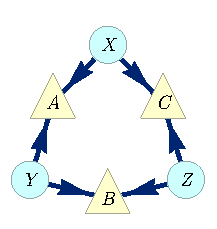
\includegraphics[scale=1]{TriDagRaw.pdf}
\caption{The causal structure of the Triangle scenario.}\label{fig:TriMainDAG}
\end{minipage}
\hfill
\begin{minipage}[t]{0.38\linewidth}
\centering
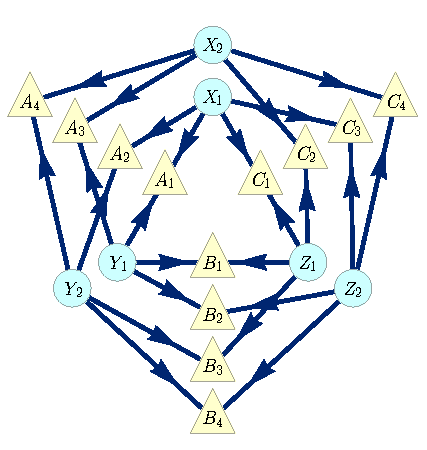
\includegraphics[scale=1]{TriDagFull222.pdf}
\caption{An inflation DAG of the Triangle scenario where each latent node has been duplicated and each observable nodes node has been quadrupled.  Note that no further duplication of observable nodes is needed, given that each has two latent nodes as parents in the original DAG and consequently there are only four possible choices of parentage of each observable node's counterpart in the inflation DAG. }\label{fig:TriFullDouble}
\end{minipage}
\hfill
\begin{minipage}[b]{0.35\linewidth}
\centering
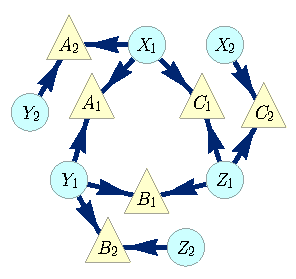
\includegraphics[scale=1]{TriDagSub222.pdf}
\caption{Another inflation of the Triangle scenario consisting, also notably $\ansubgraph[(\textrm{\cref{fig:TriFullDouble}})]{A_1 A_2 B_1 B_2 C_1 C_2}$.}\label{fig:Tri222}
\end{minipage}
\end{figure}

\begin{figure}[hb]
\centering
\begin{minipage}[t]{0.3\linewidth}
\centering
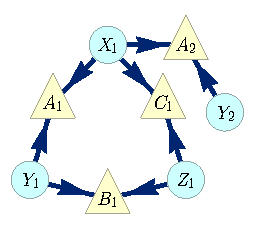
\includegraphics[scale=1]{broadcastingexamplenohighlight.pdf}
\caption{A simple inflation of the Triangle scenario, also notably $\ansubgraph[(\cref{fig:Tri222})]{A_1 A_2 B_1 C_1}$.}\label{fig:simpleinflation}
\end{minipage}\hfill
\begin{minipage}[t]{0.275\linewidth}
\centering
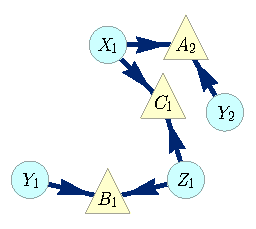
\includegraphics[scale=1]{nobroadcastingexamplenohighlight.pdf}
\caption{An even simpler inflation of the Triangle scenario, also notably $\ansubgraph[(\cref{fig:simpleinflation})]{A_2 B_1 C_1}$. }\label{fig:simplestinflation}
\end{minipage}
\hfill
\begin{minipage}[t]{0.325\linewidth}
\centering
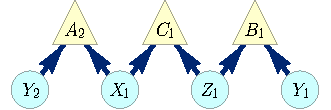
\includegraphics[scale=1]{TriDagSubA2B1C1.pdf}
\caption{Another representation of \cref{fig:simplestinflation}. Despite not containing the original scenario, this is a valid inflation per \cref{eq:definflationDAG}.}\label{fig:TriDagSubA2B1C1}
\end{minipage}
\end{figure}

We now turn to specifying the function $\SmallNamedFunction{Inflation}\;_{G\to G'}$, that is, to specifying how a causal model transforms under inflation. 
\purp{One we've said how DAG inflated, then we need TWO things: How models (and hypothesis) inflate, and also how observational data inflates. Best to word intro to subject in a way that suggests we'll be getting around to both topics sequentially?}
%Next, we turn to specifying how the parameters in the inflation of a causal model are determined from those in the original model.
%condition under which a set of parameters $\mathcal{P'}(G')$ are the inflationary image of the set of parameters $\mathcal{P}(G)$. 
\purp{PHYSICS needed here. Why mathematical abstraction? Explain that due to physical construct-ability, therefore we expect that models on the original DAG can be used to build a model on the inflation DAG...}
\begin{definition}
Consider causal models $M$ and $M'$ where $\SmallNamedFunction{DAG}{M}=G$ and $\SmallNamedFunction{DAG}{M'}=G'$ and such that $G'$ is an inflation of $G$.   The causal model $M'$ is said to be the $G\to G'$ inflation of $M$, that is, $M' = \SmallNamedFunction{Inflation}{M}$,  if and only if for every node $A_i$ in $G'$, the manner in which $A_i$ depends causally on its parents within $G'$ must be the same as the manner in which $A$ depends causally on its parents within $G$.  Noting that $A_i \sim A$ and that $\Pa[G']{A_i} \sim \Pa[G]{A}$ (given Eq.~\eqref{eq:definflationDAG}), one can formalize this condition as:
\begin{align}\label{eq:funcdependences}
%M' = \SmallNamedFunction{Inflation}{M}_{G\to G'}  \quad \text{iff}\quad 
 \forall A_i \in \SmallNamedFunction{Nodes}{G'}:\; \pfunc{A_i| \Pa[G']{A_i}}=\pfunc{A|\Pa[G]{A}},
\end{align}
%where Eq.~\eqref{eq:definflationDAG} guarantees that $A_i \sim A$ and $\Pa[G']{A_i} \sim \Pa[G]{A}$.  
\end{definition}

%A causal model specifies the causal structure and the autonomous causal mechanisms.  
To sum up then, the inflation of a causal model is a new causal model where (i) each given variable in the original DAG may have counterpart variables in the inflation DAG with ancestral subgraphs mirroring those of the originals, and (ii) where the manner in which variables depend causally on their parents in the inflation DAG is given by the manner in which their counterparts depend causally on their parents in the original DAG.   Note that the operation of modifying a DAG and equipping the modified version with conditional probability distributions that mirror those of the original also appears in the \emph{do calculus} and \emph{twin networks} of~\citet{pearl2009causality}.
%\footnote{Twin networks are similar to an inflation DAG wherein certain nodes of the original are copied, but Pearl seems to allow only two possible connections between the counterfactual twins of a given latent variable: the joint distribution over the pair of twins describes either: (i) perfect correlation, with the marginal given by the prior over that latent variable (ii) a case where the marginal on the real-world twin is given by the prior over the latent, while the counterfactual twin is fixed deterministically by an intervention.  An inflation DAG, on the other hand, corresponds  to a different option (ii) the counterfactual twins are uncorrelated, with the marginal on each twin given by the prior over the latent.}
 \fxnote{adhesivity and non-Shannon-type ineqs}
%The copying of variables under inflation implies that causal mechanisms in the inflation DAG are not necessarily autonomous, but rather often coincide with one another.


%defines a novel sort of constraint on the parameters of a causal model.  We pause to describe this constraint in general terms, before introducing the notion of inflation.  The sorts of causal structures that can arise in our inflation scheme have the property that necessarily there will be certain pairs of variables which have the same ancestral subgraph.  The constraint on the parameters is that the two conditional probability distributions describing how each variable of the pair depends on its parents are quantitatively equal to one another.  (To our knowledge, this sort of constraint has not been considered before in causal inference.)

%The inflation DAG technique that we introduce allows questions about the viability of one causal hypothesis for certain observed data to be turned into questions about the viability of a different sort of causal hypothesis for an inflation of the observed data.

%Because we have defined inflation as a map on causal models, 
Because causal hypotheses are sets of causal models, and the inflation map acts on causal models, it has an induced action on causal hypotheses.   Let $H_G^{\textsf{full}}$ denote the causal hypothesis that the DAG is $G$ (the hypothesis consisting of the set of {\em all} causal models compatible with the DAG $G$).  The induced action of the inflation map has the notable feature that $\SmallNamedFunction{Inflation}{H_G^{\textsf{full}}} \ne H_{G'}^{\textsf{full}}$ because even if there is no restriction on the set of parameters supplementing $G$, inflation imposes a restriction on the set of parameter supplementing $G'$.  Specifically,   if nodes $A_i$ and $A_j$ on $G'$ are copies of a single node $A$ on $G$,then the set of parameters on $G'$ are constrained to satisfy $\pfunc{A_i| \Pa[G']{A_i}}=\pfunc{A_j|\Pa[G']{A_j}}$.  
%This explains our earlier claim that the inflation map takes a causal hypothesis of type H1 and maps it to a causal hypothesis of type H4.

%Note that even if $S=S_{\textsf{full}}$, so that the original causal hypothesis puts no constraints on the parameter values, one generally has $S'\ne S'_{\textsf{full}}$, that is, the inflationary image of the full set of parameter values on $G$ is not the full set of parameter values on $G'$. Rather, $S'$ incorporates a nontrivial restriction on the parameters consistent with $G'$, namely, that if nodes $A_i$ and $A_j$ on $G'$ are copies of a single node $A$ on $G$,then the parameter values on $G'$ are constrained to satisfy $\pdf{A_i| \Pa[G']{A_i}}=\pdf{A_j|\Pa[G']{A_j}}$.

%Finally, we can begin to spell out how the inflation technique is useful for causal inference.  
%First, we emphasize the broad notion of causal inference that we have in mind here. 

\color{red} Why are tuples of marginals important for the problem? 

The reason inflation is useful is that there are special tuples of marginals on the distribution over the observed variables and copy-index equivalent versions of these tuples in the inflated version of the problem, such that if, in the original problem, the given tuple of marginals is compatible with the original causal hypothesis, then, in the inflated problem, any copy-index-equivalent tuple of marginals is compatible with the inflated causal hypothesis.   We demonstrate this presently. 
\color{black}

%[Note that the distinction between observed nodes and latent nodes in the DAG $G$ is inherited by the DAG $G'$.]


%It remains to explain how a $G \to G'$ inflation acts on the observational data and to prove that compatibility in the original causal decision problem implies compatibility in the image of this problem under inflation.  Both purposes are served by contemplating what inflation means for the joint distribution over observed variables induced by a causal model.  

%Because inflation is a map on causal models, it has an induced action on the joint distribution over observed variables defined by a causal model. 
%We begin by describing this action.  


%In what follows, we assume that $G$ and $G'$ are DAGs with $G' \in \SmallNamedFunction{Inflations}{G}$ and we assume that $M$ and $M'$ are causal models with $M' = \SmallNamedFunction{Inflation}{M} _{G\to G'}$.  If the joint distribution over observed variables in model $M$ is denoted by $P$, and the one in model $M'$ is denoted by $P'$.



We are now in a position to describe the key property of the inflation model, the one that makes it useful for causal inference. 
%fact that is key to understanding inflation.

Let $G$ and $G'$ be DAGs with $G' \in \SmallNamedFunction{Inflations}{G}$, let $M$ and $M'$ be causal models with $M' = \SmallNamedFunction{Inflation}{M} _{G\to G'}$, and let $P$ and $P'$ be the joint distributions over observed variables arising in models $M$ and $M'$ respectively.  For any sets of nodes $\bm{U}' \subseteq \SmallNamedFunction{Nodes}{G'}$ and   $\bm{U} \subseteq \SmallNamedFunction{Nodes}{G}$,
\begin{align}\label{eq:coincidingdistrodef}
\text{if }\quad \ansubgraph[G']{\bm{U}'}\sim\ansubgraph[G]{\bm{U}}\quad\text{then}\quad \pdfp{\bm{U}'}=\pdf{\bm{U}}.
\end{align}

This follows from the fact that the probability distributions over $\bm{U}'$ and $\bm{U}$ depend only on their ancestral subgraphs and the parameters defined thereon, which by the definition of inflation are the same for $\bm{U}'$ and for $\bm{U}$.
It is useful to have a name for those sets of observed nodes in the inflation DAG $G'$ which satisfy the antecedent of Eq.~\eqref{eq:coincidingdistrodef}, that is, for which one can find a corresponding set in the original DAG $G$ with a copy-index-equivalent ancestral subgraph.  We say that such subsets of the observed nodes of $G'$ are {\em injectable} into $G$ and we call them the \tblue{injectable sets}.  The set of all such subsets is denoted $\SmallNamedFunction{InjectableSets}{} _{G'\to G}$,
\begin{align}\label{eq:definjectable}
\bm{U}'\in\SmallNamedFunction{InjectableSets}{} _{G'\to G} \subseteq \SmallNamedFunction{ObservedNodes}{G'} \quad\text{ iff }\quad \exists \subsim{\bm{U}}\subseteq \SmallNamedFunction{ObservedNodes}{G}: \ansubgraph[G']{\bm{U}}\sim\ansubgraph[G]{\subsim{\bm{U}}}.
\end{align}

Similarly,  those sets of observed nodes in the original DAG $G$ which satisfy the antecedent of Eq.~\eqref{eq:coincidingdistrodef}, that is, for which one can find a corresponding set in the inflation DAG $G'$ with a copy-index-equivalent ancestral subgraph, we describe as {\em images of the injectable sets}, and we denote the set of these by $\SmallNamedFunction{ImagesInjectableSets}{} _{G'\to G}$.
\begin{align}\label{eq:defimageinjectable}
\bm{U}\in\SmallNamedFunction{ImagesInjectableSets}{} _{G'\to G} \quad\text{ iff }\quad \exists \bm{U}' \subseteq \SmallNamedFunction{ObservedNodes}{G'}: \ansubgraph[G']{\bm{U}}\sim\ansubgraph[G]{\subsim{\bm{U}}}.
\end{align}
Clearly, $\bm{U}\in\SmallNamedFunction{ImagesInjectableSets}{} _{G'\to G}$ iff $\exists \bm{U}' \subseteq \SmallNamedFunction{InjectableSets}{}_{G'\to G}: \b{U}\sim \bm{U}'$.


In the inflation of the triangle scenario depicted in \cref{fig:Tri222}, for example, the set of observed nodes $\brackets{A_1 B_1 C_1}$ is injectable because its ancestral subgraph is equivalent up to copy-indices to the ancestral subgraph of $\brackets{A B C}$ in the original DAG, and the set $\brackets{A_2 C_1}$ is injectable because its ancestral subgraph is equivalent to that of $\brackets{ A C}$ in the original DAG.  Note that it is clear that a set of nodes in the inflation DAG can only be injectable if it contains at most one copy of any node from the original DAG.  Similarly, it can only be injectable if its ancestral subgraph also contains at most one copy of any node from the original DAG.  
Thus, in \cref{fig:Tri222}, $\brackets{A_1 A_2 C_1}$ is not injectable because it contains two copies of $A$, and $\brackets{A_2 B_1 C_1}$ is not injectable because its ancestral subgraph contains two copies of $Y$. 

The fact that the sets $\brackets{A_1 B_1 C_1}$ and $\brackets{A_2 C_1}$ are injectable implies, via Eq.~\eqref{eq:coincidingdistrodef}, that the marginals on each of these in the inflated causal model are precisely equal to the marginals on their counterparts, $\brackets{A B C}$ and $\brackets{A C}$, in the original causal model, that is, $P'(A_1 B_1 C_1) = P(A B C)$ and $P'(A_2 C_1) = P(A C)$.

It is useful to express Eq.~\eqref{coincidingdistrodef} in the language of injectable sets, namely, as 
\begin{align}\label{keyinference}
\text{if }  \quad  \bm{U}'\in\SmallNamedFunction{InjectableSets}{} _{G'\to G} \quad \text{and} \quad \bm{U} \sim \bm{U}'  \quad\text{then}\quad \pdfp{\bm{U}'}=\pdf{\bm{U}}.
\end{align}

Finally, we can state the relevance of inflation for deciding whether a distribution is compatible with a causal hypothesis.  Consider a $G\to G'$ inflation, and suppose that some distribution $P$ is compatible with $G$, meaning that there exists a model $M$ with DAG $G$ that yields the distribution $P$.  It follows that the set of marginals of $P$ on the images of the injectable sets, that is, $\{ P(\bm{U}) : \bm{U} \in \SmallNamedFunction{ImagesInjectableSets}{}_{G'\to G}$ is also compatible with $G$.  But then, by Eq.~\eqref{keyinference}, there is a distribution $P'$ compatible with $G'$ (the one associated to the causal model $M' = \SmallNamedFunction{Inflation}{M}_{G' \to G}$) such that for each $\bm{U}'\in\SmallNamedFunction{InjectableSets}{} _{G'\to G}$, $P'(\bm{U}') = P(\bm{U})$, and therefore the set $\{ P'(\bm{U}') : \bm{U}' \in \SmallNamedFunction{InjectableSets}{}_{G'\to G} \}$ is compatible with $G'$.

We formalize the result as a lemma. 
\begin{lemma} Let $G$ and  $G'$ be DAGs with $G'$ an inflation of $G$.   If the set of distributions $\{ P(\bm{U}) : \bm{U} \in \SmallNamedFunction{ImagesInjectableSets}{}_{G'\to G} \}$ is compatible with $G$, then the set of distributions $\{ P'(\bm{U}') : \bm{U}' \in \SmallNamedFunction{InjectableSets}{}_{G'\to G} \}$ is compatible with $G'$.
\end{lemma}

We have thereby converted a question about compatibility for the original causal structure to one about compatibility for the inflated causal structure.  If one can show that the new compatibility question is answered in the negative, one can infer that the original question is answered in the negative as well.    Some simple examples serve to illustrate the idea. 
%We now provide some simple examples of applications of this result.


%Therefore, if $P$ denotes a distribution over the observed variables of the Triangle scenario and $P'$ a distribution over the observed variables of the DAG \cref{fig:Tri222}, 

\color{red}
New narrative.

Here is the key idea: for a certain DAG, a particular tuple of marginals will generally be constrained, but it is difficult to determine precisely how they are constrained.  It is easy, however, to construct a new DAG and a new tuple of marginals, where some of the elements of the tuple are by construction equal and where the independent elements of the tuple are isomorphic to those of the original problem and where by construction the tuple of independent marginals satisfies precisely the same constraints in the new problem as in the old.   
Deriving constraints in this new context can be much more straightforward.  Typically, we find that we can ignore the equality condition and just apply some naive sorts of constraints, like those that follow from ancestral independence, and obtain some nontrivial constraints.   The fact that the new DAG has a richer structure tends to make for more such opportunites for easy constraints. 

For example, the tuple of marginals $(P(B_1), P(C_1), P(B_1 A_1), P(A_1 C_1))$ in the inflation of the triangle DAG which duplicates Y is constrained because the marginals problem dictates a nontrivial relation among $(P(B_1,C_1), P(B_1 A_1), P(A_1 C_1))$ (having nothing to do with causal structure) and then the causal structure implies that $P(B_1,C_1) = P(B_1)P(C_1)$, which when substituted into the relation gives a constraint that does follow from causal structure.  This inequality encodes the presence of the ancestral independence relation.  (But of course it encodes nothing more than is encoded by saying that $B_1$ and $C_1$ are marginally independent---it is only when combined with the inflation technique that it is useful.)

But this tuple of marginals provably satisfies the same constraints as the tuple  $(P(B), P(C), P(B A), P(A C))$ in the triangle.  (This can be seen as follows: every quantifier elimination problem in the original problem looks exactly the same as in the new problem, regardless of the dimensionality of the latent varaibles, and therefore independently of any assumptions about that dimensioanlity)

A given joint distribution being compatible with the original causal hypothesis does not imply that it is compatible with the inflated causal hypothesis.  Indeed, the observed variables are not even the same in the two cases.   However, certain tuples of marginals being compatible with the original causal hypothesis do imply that an inflation of the tuple of marginals (where each marginal now applies to the copy-index-equivalent variables in the inflated DAG) is compatible with the inflated causal hypothesis.  

Thus any tricks that can be used to infer incompatibility or provide a necessary condition for compatibility of the inflated tuple of marginals with the inflated causal hypothesis can be used to infer incompatibility or provide a necessary condition for compatibility of the original causal inference problem.

\color{black}
\section{Deciding compatibility using the Inflation technique}


\color{red}
[Define notational convention of $[x]$]
\color{black}

\example{: \tred{Perfect three-way correlation is incompatible with the Triangle scenario.}}\par\smallskip\nobreak

\color{red} [Move the relevant figure here.  Put the triangle and its inflation side by side.  I think it's okay to repeat the triangle DAG in our figures.]\color{black}


Consider the following causal inference problem.  One is given a joint distribution over three binary variables, $P_{A B C}$, where the marginal on each variable is uniform and the three are perfectly correlated,
\begin{align}\label{eq:ghzdistribution1}
P_{A B C} =\frac{[000]+[111]}{2},\quad\text{i.e.}\quad P_{A B C}(a b c)=\begin{cases}\tfrac{1}{2}&\text{if }\; a\eql b\eql c, \\ 0&\text{otherwise}.\end{cases}
\end{align}
%The causal hypothesis is the set of causal models associated to the DAG
The causal hypothesis is that the DAG corresponds to the triangle scenario, depicted in \cref{fig:Tri222}.  The problem is to decide whether the given distribution is compatible with this causal hypothesis.


To solve this problem, we consider the inflation of the triangle scenario to the DAG depicted in Fig.~\ref{fig:TriDagSubA2B1C1}.  
The injectable sets in this case include $\brackets{A_2 C_1}$ and $\brackets{B_1 C_1}$.  We therefore consider the marginals on these sets.

Clearly, the given distribution is compatible with the triangle hypothesis, only if the following pair of marginals of the given distribution are compatible with the triangle hypothesis:
\begin{align}
%\label[eqs]{eq:GHZobsinf}
P_{A C} &= \frac{[00]+[11]}{2}\label{j1}\\
P_{B C} &= \frac{[00]+[11]}{2}\label{j2}
\end{align}
But by lemma ??, this compatibility holds only if the following pair of marginals is compatible with the inflation DAG depicted in Fig.~\ref{fig:TriDagSubA2B1C1}:
\begin{align}
P_{A_2 C_1} &= \frac{[00]+[11]}{2} \label{k1}\\
P_{B_1 C_1} &= \frac{[00]+[11]}{2} \label{k2}
\end{align}


It is not difficult to see that the latter pair of marginals is \emph{not} compatible with our inflation DAG. It suffices to note that the only joint distribution that exhibits perfect correlation between $A_2$ and $C_1$ and between $B_1$ and $C_1$ also exhibits perfect correlation between $A_2$ and $B_1$.  But $A_2$ and $B_1$ have no common ancestors and hence must be marginally independent in the inflation DAG.

We have therefore certified that the joint distribution $P_{A B C}$ of Eq.~\eqref{eq:ghzdistribution1} is not compatible with the Triangle causal structure, recovering the seminal result of \citet{steudel2010ancestors}.

\begin{comment}
Let us ask, is it possible for the three original-scenario observable variables $\{A,B,C\}$ to be random but perfectly correlated? We call this the GHZ-type distribution, after an eponymous tripartite entangled quantum state \cite{greenberger1989going,3Qubits2Ways}. So $P_{\text{GHZ}}\parenths{A B C}$ is given by
\begin{align}\label{eq:ghzdistribution1}
p_{\text{GHZ}}\parens{a b c}=\frac{[000]+[111]}{2}=\begin{cases}\tfrac{1}{2}&\text{if }\; a=b=c, \\ 0&\text{otherwise}.\end{cases}
\end{align}
We assume uniform binary variables for the sake of concreteness, but the argument is general. Let's temporarily (falsely) assume $P_{\text{GHZ}}$ to be compatible with the triangle scenario. Since $\brackets{A_2 C_1}$ is an injectable set we have $\pdf{A_2 C_1}=\pdf{A C}$, and therefore $P_{\text{GHZ}}$ implies that $A_2$ and $C_1$ are perfectly correlated. Similarly, since $\brackets{B_1 C_1}$ is an injectable set we have $\pdf{B_1 C_1}=\pdf{A C}$, and therefore $B_1$ and $C_1$ must be perfectly correlated, and by extension $B_1$ and $A_2$ are perfectly correlated as well. On the other hand, $A_2$ and $B_1$ must be statistically independent, as they do not share any common ancestor. The only way for two variables to be \emph{both} perfectly correlated and independent is by being deterministic. This is not the case in $P_{\text{GHZ}}$, and thus we have certified that $P_{\text{GHZ}}$ is not realizable from the Triangle causal structure, recovering the seminal result of \citet{steudel2010ancestors}.
\end{comment}

\example{: \tred{The W-type distribution is incompatible with the Triangle scenario}}\par\smallskip\nobreak

\color{red} [Move the relevant figure here.  Put the triangle and its inflation side by side.  I think it's okay to repear the triangle DAG in our figures.]\color{black}

Consider another causal inference problem concerning the triangle scenario, namely, that of determining whether the hypothesis of the triangle DAG is compatible with a joint distribution 
%$P^{\text{W}}_{A B C}$
$P_{A B C}$ of the form
\begin{align}\label{eq:wdistribution1}
P_{A B C}=\frac{[100]+[010]+[001]}{3},\quad\text{i.e.}\quad P_{A B C}(a b c)=\begin{cases}\tfrac{1}{3}&\text{if }\; a\cramp{+}b\cramp{+}c\eql 1, \\ 0&\text{otherwise}.\end{cases}
\end{align}
We call this the W-type distribution\footnote{Because its correlations are reminiscent of those one obtains for the quantum state appearing in Ref. \cite{3Qubits2Ways}, and which is called the W state.}. 
%To our knowledge, the fact that the Triangle causal structure is inconsistent with the W-type distribution has not been demonstrated previously.

To settle the compatibility question, we consider the inflation DAG of \cref{fig:Tri222}.  The injectable sets in this case include $\{ A_1 B_1 C_1\}$, $\{A_2 C_1\}$, $\{B_2 A_1\}$, $\{A_2 B_1\}$,  $\{ A_2\}$, $\{B_2\}$ and $\{C_2\}$. 

Therefore, we turn our attention to the problem of whether the following set of marginals of the W-type distribution is compatible with the triangle hypothesis:
\begin{align}
P_{A B C}&= \frac{[100]+[010]+[001]}{3} &&&&&&&&\label{V4}\\
P_{A C}&= \frac{[10]+[01]+[00]}{3} &&&&&&&&\label{V1}\\
P_{B A}&=\frac{[10]+[01]+[00]}{3} &&&&&&&&\label{V2}\\
P_{C B}&= \frac{[10]+[01]+[00]}{3} &&&&&&&&\label{V3}\\
P_{A}&= \frac{2}{3}[0] + \frac{1}{3}[1] &&&&&&&&\label{V5}\\
P_{B}&=\frac{2}{3}[0] + \frac{1}{3}[1]  &&&&&&&&\label{V6}\\
P_{C}&= \frac{2}{3}[0] + \frac{1}{3}[1]  &&&&&&&&\label{V7}
\end{align}

But by lemma ??, this compatibility holds only if the following set of marginals is compatible with the inflation DAG depicted in Fig.~\ref{fig:TriDagSubA2B1C1}:
\begin{align}
P_{A_1 B_1 C_1}&= \frac{[100]+[010]+[001]}{3} &&&&&&&&\label{W4}\\
P_{A_2 C_1}&= \frac{[10]+[01]+[00]}{3} &&&&&&&&\label{W1}\\
P_{B_2 A_1}&=\frac{[10]+[01]+[00]}{3} &&&&&&&&\label{W2}\\
P_{C_2 B_1}&= \frac{[10]+[01]+[00]}{3} &&&&&&&&\label{W3}\\
P_{A_2}&= \frac{2}{3}[0] + \frac{1}{3}[1] &&&&&&&&\label{W5}\\
P_{B_2}&=\frac{2}{3}[0] + \frac{1}{3}[1]  &&&&&&&&\label{W6}\\
P_{C_2}&= \frac{2}{3}[0] + \frac{1}{3}[1]  &&&&&&&&\label{W7}
\end{align}

Eq.~\eqref{W1} %together with the form of $P_{\text{W}}$ 
implies that $C_1\eql 0$ whenever $A_2 \eql 1$. Similarly, Eq.~\eqref{W2} implies that $A_1\eql 0$ whenever $B_2\eql 1$ and Eq.~\eqref{W3} implies that $B_1\eql 0$ whenever $C_2\eql 1$, 
%, that is, $A_2=1$ and $B_2=1$ and $C_2=1$.  
%Summarizing, we have
\begin{align} 
&A_2 \eql 1 \implies C_1\eql 0\label{Ws1}\\
&B_2\eql 1 \implies A_1\eql 0\label{Ws2}\\
&C_2 \eql 1 \implies B_1 \eql 0\label{Ws3}
\end{align}

Our inflation DAG is such that $A_2$,$B_2$, and $C_2$ have no common ancestor and consequently, they are all marginally independent in any distribution consistent with this inflation DAG.  This fact, together with Eqs.~\eqref{W5}-\eqref{W7}, implies that $A_2$,$B_2$, and $C_2$ sometimes all take the value 1,
\begin{align} \label{WW2}
\text{Sometimes} \quad &A_2 \eql 1, B_2 \eql 1, C_2 \eql 1.
\end{align} 

Finally, Eqs.~\eqref{Ws1}-\eqref{Ws3} together with Eq.~\eqref{WW2} imply
\begin{align} \label{WW3}
\text{sometimes} \quad &A_1 \eql 0, B_1 \eql 0, C_1 \eql 0.
\end{align}
This, however, contradicts Eq.~\eqref{W4}.  Consequently, the set of marginals described in Eqs.~\eqref{W4}-\eqref{W7} are \emph{not} compatible with the DAG of Fig.~\ref{fig:TriDagSubA2B1C1}.  By lemma ??, this implies that the set of marginals described in Eqs.~\eqref{V4}-\eqref{V7}---and therefore the W-type distribution of which they are marginals---is not compatible with the DAG of the triangle scenario.
% and the fact that $P_{\text{W}}$ has no weight on $[000]$.

We have secured our verdict of incompatability using logic reminiscent of  Hardy's version of Bell's theorem \cite{L.Hardy:PRL:1665,Mansfield2012}, see \cref{sec:TSEM} for further discussion of Hardy-type paradoxes and their applications.

To our knowledge, the fact that the W-type distribution of Eq.~\eqref{eq:wdistribution1} is incompatible with the triangle DAG has not been demonstrated previously.

%$\p{A_2\eql B_2\eql C_2\eql 1}=\nicefrac{1}{8}$ according to $P_{\text{W}}$. But that would imply $\p{A_1\eql B_1\eql C_1\eql 0}\geq\nicefrac{1}{8}$, which contradicts $P_{\text{W}}$, hence $P_{\text{W}}$ cannot arise from the Triangle scenario.

The incompatibility of the triangle DAG with the W-type distribution is difficult to infer from conventional causal inference techniques.
\begin{compactenum}
\item There are no conditional independence relations between the observable nodes of the Triangle scenario. %, so the distribution is observationally Markov with respect to the DAG. 
\item Shannon-type entropic inequalities cannot detect this distribution as not allowed by the Triangle scenario~\cite{fritz2013marginal,chaves2014novel,chaves2014informationinference}. 
\item Moreover, \emph{no} entropic inequality can witness the W-type distribution as unrealizable. \citet{weilenmann2016entropic} have constructed an inner approximation to the entropic cone of the Triangle causal structure, and the W-distribution lies inside this. In other words, a distribution with the same entropic profile as the W-type distribution \emph{can} arise from the Triangle scenario.
\item The newly-developed method of covariance matrix causal inference due to \citet{kela2016covariance}, which gives tighter constraints than entropic inequalities for the Triangle scenario, also cannot detect incompatibility with the W-type distribution.
\end{compactenum}
%\par\noindent But the inflation technique can, and does so very easily.
Therefore, for this problem at least, the inflation technique appears to be more powerful.

\example{: \tred{PR-box correlations are incompatible with the Bell scenario}}\par\smallskip\nobreak

Bell's theorem concerns whether the distribution obtained in an experiment involving a pair of systems that are measured at space-like separation \cite{bell1964einstein,Brunner2013Bell,bell1966lhvm,CHSHOriginal} is compatible with a causal structure of the form of \cref{fig:NewBellDAG1}, as has been noted in several recent articles \cite{bell1964einstein,Brunner2013Bell,bell1966lhvm,CHSHOriginal} scenario [\citealp{pusey2014gdag}~(Fig.~E\#2), \citealp{WoodSpekkens}~(Fig.~19), \citealp{chaves2014novel}~(Fig.~1), \citealp{BeyondBellII}~(Fig.~1), \citealp{wolfe2015nonconvexity}~(Fig.~2b), \citealp{steeg2011relaxation}~(Fig.~2)].  Here, the observed variables are $\brackets{A,B,X,Y}$, and $\Lambda$ is a latent variable acting as a common cause of $A$ and $B$.   We shall term this causal structure the \emph{Bell scenario}.

%Consider the causal structure associated to the Bell \cite{bell1964einstein,Brunner2013Bell,bell1966lhvm,CHSHOriginal} scenario [\citealp{pusey2014gdag}~(Fig.~E\#2), \citealp{WoodSpekkens}~(Fig.~19), \citealp{chaves2014novel}~(Fig.~1), \citealp{BeyondBellII}~(Fig.~1), \citealp{wolfe2015nonconvexity}~(Fig.~2b), \citealp{steeg2011relaxation}~(Fig.~2)], depicted here in \cref{fig:NewBellDAG1}. The observable variables are $\brackets{A,B,X,Y}$, and $\Lambda$ is the latent common cause of $A$ and $B$. 

\begin{figure}[ht]
\centering
\begin{minipage}[t]{0.45\linewidth}
\centering
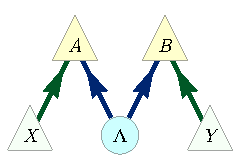
\includegraphics[scale=1]{BellDagRaw.pdf}
\caption{The causal structure of the a bipartite Bell scenario. The local outcomes of Alice's and Bob's experimental probing is assumed to be a function of some latent common cause, in addition to their independent local experimental settings.}\label{fig:NewBellDAG1}
\end{minipage}
\hfill
\begin{minipage}[t]{0.45\linewidth}
\centering
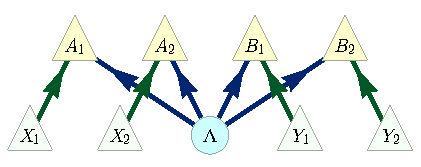
\includegraphics[scale=1]{BellDagCopy.pdf}
\caption{An inflation DAG of the bipartite Bell scenario, where both local settings variables have been duplicated.}\label{fig:BellDagCopy1}
\end{minipage}
\end{figure}

%P^{\text{obs-inf}}_{A_2 C_1}

We consider the distribution ${P_{A B X Y} = P_{A B | X Y} \otimes P_{X} \otimes P_{Y}}$, where $P_{X}$ and $P_{Y}$ are arbitrary full-support distributions\footnote{In the literature on the Bell scenario, these variables are known as ``settings''. Generally, we may think of endogenous observable variables as settings, coloring them light green in the DAG figures. Settings variables are natural candidates for conditioning on.} over the binary variables $X$ and $Y$, and
\begin{align}\begin{split}\label{eq:PRbox}
% & p_{\text{PR}}\parens{a b |x y}=\frac{[00|00]+[11|00]+[00|10]+[11|10]+[00|01]+[11|01]+[01|11]+[10|11]}{8}\\
P_{A B | X Y}\parens{a b |x y}=\begin{cases}\tfrac{1}{2}&\text{if }\; \SmallNamedFunction[2]{mod}{a\cramp{+}b}\eql x\cramp{\cdot} y, \\ 0&\text{otherwise}.\end{cases}
\end{split}\end{align}
The correlations described by this distribution are known as PR-box correlations after Popescu and Rohrlich, and they are well-known to be incompatible with the the Bell scenario \cite{PROriginal,PRUnit}. Here we prove this incompatibility using the inflation technique. 

We use the inflation of the Bell DAG shown in \cref{fig:BellDagCopy1}.

We begin by noting that $\{A_1 B_1 X_1 Y_1\}$, $\{A_2 B_1 X_2 Y_1\}$, $\{A_1 B_2 X_1 Y_2\}$, $\{A_2 B_2 X_2 Y_2\}$, $\{X_1\}$, $\{X_2\}$, $\{Y_1\}$, and $\{Y_2\}$ are all injectable sets. 
By lemma ??, it follows that 
\begin{align}
P_{A_1 B_1 X_1 Y_1}&=P_{A B X Y}\label{PR1}\\
P_{A_2 B_1 X_2 Y_1}&=P_{A B X Y}\label{PR2}\\
P_{A_1 B_2 X_1 Y_2}&=P_{A B X Y}\label{PR3}\\
P_{A_2 B_2 X_2 Y_2}&=P_{A B X Y}\label{PR4}\\
P_{X_1}&=P_X\label{PR5}\\
P_{X_2}&=P_X\label{PR6}\\
P_{Y_1}&=P_Y\label{PR7}\\
P_{Y_2}&=P_Y\label{PR8}.
\end{align}
Using the definition of conditional probability, we infer that
\begin{align}
P_{A_1 B_1 |X_1 Y_1}&=P_{A B |X Y}\label{PR1b}\\
P_{A_2 B_1 |X_2 Y_1}&=P_{A B |X Y}\label{PR2b}\\
P_{A_1 B_2 |X_1 Y_2}&=P_{A B |X Y}\label{PR3b}\\
P_{A_2 B_2 |X_2 Y_2}&=P_{A B |X Y}\label{PR4b}.
\end{align}


Because $\{X_1\}$, $\{X_2\}$, $\{Y_1\}$, and $\{Y_2\}$ have no common ancestor, these variables must be marginally independent in any distribution compatible with the inflation DAG,  that is, we have $P_{X_1 X_2 Y_1 Y_2} = P_{X_1} P_{X_2} P_{Y_1} P_{Y_2}$ in any such distribution.   Given the assumption that the distributions $P_{X}$ and $P_{Y}$ are full support, it follows from Eqs.~\eqref{PR5}-\eqref{PR8} that
\begin{align}\label{PRs}
\text{Sometimes} \quad &X_1 \eql 0, X_2 \eql1, Y_1 \eql 0, Y_2 \eql 1.
\end{align} 

Next, from Eqs.~\eqref{PR1b}-\eqref{PR4b} together with  the definition of PR box correlations, Eq.~\eqref{eq:PRbox}, we conclude that 
\begin{align} 
&X_1 \eql 0, Y_1 \eql 0 \implies A_1\eql B_1 \label{PRs1},\\
&X_1 \eql 0, Y_2 \eql 1 \implies A_1\eql B_2 \label{PRs2},\\
&X_2 \eql 1, Y_1 \eql 0 \implies A_2\eql B_1 \label{PRs3},\\
&X_2 \eql 1, Y_2 \eql 1 \implies A_2\ne B_2 \label{PRs4}.
\end{align}

Combining Eq.~\eqref{PRs} with Eqs,~\eqref{PRs1}-\eqref{PRs4}, we obtain
\begin{align}\label{PRs}
\text{Sometimes} \quad &A_1\eql B_1, A_1\eql B_2, A_2\eql B_1, A_2\ne B_2.
\end{align} 
No values of $A_1, A_2, B_1, B_2$ can jointly satisfy these conditions---the first three properties entail perfect correlation between $A_2$ and $B_2$---so we have reached a contradiction.

%For these values, \cref{eq:PRinflated} specifies perfect correlation between $A_1$ and $B_1$.  Similarly, it the inflated observational data also specified perfect correlation between $A_1$ and $B_2$, perfect correlation between $A_2$ and $B_1$, and perfect \emph{anti}correlation between $A_2$ and $B_2$. Those four requirements are not mutually compatible, however: since perfect correlation is transitive, the first three properties entail perfect correlation between $A_2$ and $B_2$. 

The mathematical structure of this proof parallels that of standard proofs of the incompatibility of PR-box correlations with the Bell DAG.  Standard proofs focus on a set of variables $\{A_0, A_1, B_0, B_1\}$ where $A_0$  is the value of $A$ when $X=0$, and similarly for the others. They note that if the Bell DAG describes the experiment, then by taking the product of the conditional of $A_0$ given $\lambda$ with the conditional of $A_1$ given $\lambda$, etcetera, one obtains a joint distribution over $\{A_0, A_1, B_0, B_1\}$ for which the marginals on pairs  $\{ A_0, B_0\}$, $\{ A_0, B_1\}$, $\{ A_1, B_0\}$ and $\{ A_1, B_1\}$ are those predicted by the causal model.  Finally, these marginals are shown to satisfy a Bell inequality, while the PR box correlations are shown to violate this inequality.   \purp{Is there a ``standard proof'' that excludes PR box without referring to Bell inequalities? Say something about the difference of the standard approach to our approach?---RWS}

% The fact that there must be a joint distribution over these variables can be inferred from the structure of the Bell DAG and the fact that one can assume without loss of generality that the causal dependences are deterministic (a result known as Fine's theorem \cite{FineTheorem}).  It is then sufficient to note that the marginals given by the PR-box correlations do not arise from any joint distribution.  Nonetheless, our proof is conceptually distinct insofar as the variables to which we apply the marginals problem are not conditioned on a setting value.  And we do not require Fine's theorem.  

%Many causal inference techniques can be used to derive sufficient conditions for the incompatibility of the causal hypothesis $H_{G',S'}$ with the observational data $\forall \bm{U} \in \SmallNamedFunction{PreInjectableSets}{\bm{O}}: \pdf{\bm{U}} = \pdf{\subsim{\bm{U}_1}}\pdf{\subsim{\bm{U}_2}} \dots \pdf{\subsim{\bm{U}_n}}$. We will call sets of such conditions \tblue{incompatibility witnesses}.   

\color{black}

\section{Deriving causal compatibility inequalities using the inflation technique}

\color{blue}
As noted in the introduction, the inflation technique can be used not only to render verdicts on the compatibility of a given distribution with a given causal structure, but it can also be used to derive necessary conditions that a distribution must satisfy to be compatible with the given causal structure.   When these necessary conditions are as inequalities, we will refer to them as {\em causal compatibility inequalities}.


%The relation between nodes of the inflation DAG $G'$ to nodes on the DAG $G$ that will be of primary interest to us is not injectability  actually slightly weaker than the notion of injectability.  
The sets of nodes of $G'$ that will be of primary interest to us are not the injectable sets per se, but sets satisfying a slightly weaker constraint.
%We call this notion {\em pre-injectability}.  
To define the latter sorts of sets, which we term {\em pre-injectable}, we must first introduce some additional terminology. 

We refer to a pair of nodes which do not share any common ancestor as being \tblue{ancestrally independent}, for which we invent the notation $X\aindep Y$. Generalizing to sets, $\bm{U}\aindep \bm{V}$ indicates that no node in $\bm{U}$ shares a common ancestor with any node in $\bm{V}$, 
\begin{align}
\bm{U}\aindep \bm{V} \quad \text{iff} \quad \An{\bm{U}}\cap\An{\bm{V}}=\emptyset.
\end{align}
%i.e.~$\An{\bm{U}}\cap\An{\bm{V}}=\emptyset$. 
%It is possible for more than two sets to be ancestrally independent: the notation ${\bm{U}\aindep \bm{V}\aindep \bm{W}}$ should be understood as indicating that the ancestors of $\bm{U}$,$\bm{V}$, and $\bm{W}$ comprise three distinct non-overlapping sets, i.e.~$\bm{U}\aindep \bm{V}$ and $\bm{V}\aindep \bm{W}$ and $\bm{U}\aindep \bm{W}$.
Ancestral independence is equivalent to $d$-separation by the empty set~\cite{pearl2009causality,spirtes2011causation,studeny2005probabilistic,koller2009probabilistic}. 


A set of nodes $\bm{U}$ in the inflation DAG $G'$ will be called \tblue{pre-injectable} whenever it is a union of injectable sets with disjoint ancestries. 
\begin{align}\label{eq:defpreinj}
\bm{U}\in\SmallNamedFunction{PreInjectableSets}{G'} \quad\text{ iff }\quad  \exists \{ \bm{U}_i \in \SmallNamedFunction{InjectableSets}{G'} \} \quad \text{s.t.}\quad \bm{U}=\bigcup_i \bm{U}_i  \quad\text{and} \quad  \forall i\ne j: \bm{U}_i \aindep \bm{U}_j.
%\bm{U}\in\SmallNamedFunction{PreInjectableSets}{G'} \quad\text{ iff }\quad  \exists \{ \bm{U}_i \}_i \quad \text{s.t.}\quad \bm{U}=\bigcup_i \bm{U}_i  \quad\text{and} \quad \forall i 
%: \bm{U}_i \in \SmallNamedFunction{InjectableSets}{G'}\quad \text{and}\quad \forall i,j
%: \bm{U}_i \aindep \bm{U}_j.
\end{align}
%Equivalently, a set of nodes is pre-injectable if and only if its (weakly) connected components are injectable. 
Note that every injectable set is a trivial example of a pre-injectable set.

Because ancestral independence in the DAG implies statistical independence for any probability distribution compatible with the DAG, it follows that  if 
$\bm{U}$ is a pre-injectable set and $\bm{U}_1,\bm{U}_2,\ldots,\bm{U}_n$ are the ancestrally independent components of $\bm{U}$, then 
\begin{align}%\label{eq:preinjfactor}
%\forall \bm{U}\in\SmallNamedFunction{PreInjectableSets}{G'}:	
\pdfp{\bm{U}} = \pdfp{\bm{U}_1} \pdfp{\bm{U}_2}  \cdots \pdfp{\bm{U}_n}.
\end{align}
Furthermore, because each injectable set of variables $\bm{U}_i$ satisfies Eq.~\eqref{eq:coincidingdistrodef}, it follows that joint distributions on pre-injectable sets in the inflation model can be expressed in terms of distributions defined on the original causal model,
\begin{align}\label{eq:preinjfactor}
%\forall \bm{U}\in\SmallNamedFunction{PreInjectableSets}{G'}:	
\pdfp{\bm{U}} = \pdf{\subsim{\bm{U}}_1} \pdf{\subsim{\bm{U}}_2}  \cdots \pdf{\subsim{\bm{U}}_n}.
\end{align}
This relation specifies precisely how the marginal distribution over any pre-injectable set in the inflated causal model is defined in terms of the distribution over the corresponding set of variables in the original causal model. 

%This latter property implies that the observable probability distribution over any pre-injectable set in the inflation model is fully specified by the \sout{parameters} \purp{observable probability distribution} \sout{in the original causal model} \purp{per the original observable data}.  Indeed, this relation is what motivates us to consider the pre-injectable sets.

Because this relation involves only {\em observed variables} of the original and inflated causal models, one can use it to determine observational constraints for the inflated causal inference problem from observational constraints for the original problem. 
% define the consequences of the inflation map on the observational constraints.   

In the original causal inference problem, whatever form the observational constraint takes, one can deduce its consequences for the marginals on subsets of variables that correspond to injectable sets with copy-indices dropped, that is, the marginals on subsets $\subsim{\bm{U}}\subseteq \SmallNamedFunction{ObservedNodes}{G}$ satisfying $\subsim{\bm{U}} \sim \bm{U}$ where $\bm{U} \in  \SmallNamedFunction{InjectableSets}{G'}$.  Marginalization onto $\subsim{\bm{U}}$ is a map on probability distributions, but given that the observational constraint $D^{\textrm{obs}}$ is a set of probability distributions, such marginalization has an induced action on $D^{\textrm{obs}}$.  We denote the marginalization onto $\subsim{\bm{U}}$ of $D^{\textrm{obs}}$ by $D_{\subsim{\bm{U}}}^{\textrm{obs}}$.   The set $D_{\subsim{\bm{U}}}^{\textrm{obs}}$ captures the consequences of the observational constraints for the marginal distribution on $\subsim{\bm{U}}$.


%over the observed variables.  Consider a set of observed variables $\subsim{\bm{U}}\subseteq \SmallNamedFunction{ObservedNodes}{G}$ satisfying $\subsim{\bm{U}} \sim \bm{U}$ where $\bm{U} \in  \SmallNamedFunction{InjectableSets}{G'}$.  For each joint distribution over the observed variables, $P^{\rm obs}(\SmallNamedFunction{ObservedNodes}{G})$, marginalization on $\subsim{\bm{U}}$ defines a distribution $P^{\rm obs}(\subsim{\bm{U}})$.  The observational constraint $D^{\rm obs}$ specifies a set of possibilities for the joint distribution.  The image of this set under marginalization on $\subsim{\bm{U}}$ we denote by $D_{\subsim{\bm{U}}}^{\rm obs}$.

%Similarly, in the inflated causal inference problem, if we consider a set of observed variables $\bm{U} \in  \SmallNamedFunction{PreInjectableSets}{G'}$ and we consider .  For each joint distribution over the observed variables, $P^{\rm obs}(\SmallNamedFunction{ObservedNodes}{G})$, marginalization on $\subsim{\bm{U}}$ defines a distribution $P^{\rm obs}(\subsim{\bm{U}})$.  
In the inflated causal inference problem, suppose the observational constraint $D'^{\textrm{obs}}$ specifies a set of possibilities for the joint distribution on $\SmallNamedFunction{ObservedNodes}{G'}$.  For every pre-injectable set $\bm{U} \in  \SmallNamedFunction{PreInjectableSets}{G'}$, let the image of $D'^{\textrm{obs}}$ under marginalization on $\subsim{\bm{U}}$ be denoted by $D_{\subsim{\bm{U}}}^{\prime \textrm{obs}}$.  It is then clear from Eq.~\eqref{eq:preinjfactor} that if $\bm{U}_1,\bm{U}_2,\ldots,\bm{U}_n$ are the ancestrally independent components of $\bm{U}$, as in Eq.~\eqref{eq:defpreinj}, then
\begin{align}%\label{eq:preinjfactor}
\forall \bm{U} \in  \SmallNamedFunction{PreInjectableSets}{G'}:  D_{\subsim{\bm{U}}}^{\prime \textrm{obs}} \equiv \{ \pdfp{\bm{U}} = \prod_i \pdf{\subsim{\bm{U}}_i}: \pdf{\subsim{\bm{U}}_i} \in D_{\subsim{\bm{U}_i}}^{\textrm{obs}}\quad \forall i \}.
\end{align}




%we denote the subset of distributions $\pdf{\subsim{\bm{U}}}$ that can arise by marginalization from the subset of joint distributions defined by $D^{\rm obs}$ as $D_0^{\rm obs}$.  

%We denote the the observational constraints by $D_0^{\rm obs}$.  They are:
%\begin{align}
%D_0^{\rm obs} \equiv \{ \pdf{\subsim{\bm{U}}} : \subsim{\bm{U}} \sim \bm{U} \in  \SmallNamedFunction{InjectableSets}{G'}, \text{marginals of}\quad\pdf{\SmallNamedFunction{ObservedNodes}{G}}  \in D^{\rm obs} \}
%\end{align}
The key is this: if a given specification of marginals on deflated injectables is compatible with the original causal hypothesis, then the corresponding products of marginals on the pre-injectable sets is compatible with the inflated causal hypothesis.  If a joint distribution is compatible with the original causal hypothesis, then its marginals on deflated injectables are as well, and we get the corresponding inference on the inflated problem.  An observational constraint provides a bunch of joint distribution candidates for compatibility with the causal hypothesis and inflation turns these into a bunch of marginals candidates for compatibility with the inflated causal hypothesis. 

If the observational constraint $D^{\textrm{obs}}$ and the causal hypothesis $H_G$ are compatible, then the observational constraint $\{  D_{\subsim{\bm{U}}}^{\prime \textrm{obs}} : \bm{U} \in  \SmallNamedFunction{PreInjectableSets}{G'}\}$ and the causal hypothesis $H_{G'} = \SmallNamedFunction{Inflation}{H_G}$ are compatible.  

We need to define the notion of observational constraints on a set of marginal distributions.  Let $\SmallNamedFunction{Subsets}{G}$ be the subsets of the nodes of $G$ on which we impose our observational constraints.  Let $( P(\bm{U}): U \in \SmallNamedFunction{Subsets}{G} )$ be a collection of marginals associated to these subsets.  Then the observational constraint on marginals is a set of such collections, denoted $D^{\textrm{obs}}_{\textrm{marg}}$.
%\begin{align}
%D^{\rm obs}_{\rm marg} \equiv  \{ ( P(\bm{U}): U \in \SmallNamedFunction{Subsets}{G} ) 
%\end{align}

Let the function $\SmallNamedFunction{JointDistObserved}{M}$ return the joint distribution over the observed nodes implied by causal model $M$, via Eqs. ???.

Compatibility in the original causal inference problem implies that 
\begin{align}
\exists M \in H_G : \SmallNamedFunction{JointDistObserved}{M} \in D^{\textrm{obs}}
\end{align}
  


%So to witness the incompatibility of $D^{\rm obs}$ and $H_G$, it is sufficient to witness the incompatibility 
\begin{comment}
\color{red}
We can now describe the image of the observational constraint $D^{\textrm{obs}}$ under the $G\to G'$ inflation map, $D'^{\textrm{ obs}}=\SmallNamedFunction{Inflation}{D^{\textrm{obs}}} _{G\to G'}$, as follows:
\begin{align}
D'^{\textrm{obs}} \equiv \{ \pdf{all} : \text{marginals}  \pdf{\subsim{\bm{U}}} : \subsim{\bm{U}} \sim \bm{U} \in  \SmallNamedFunction{InjectableSets}{G'} \text{are built from } D_0^{\textrm{obs}} \text{via Eq.~\eqref{eq:preinjfactor}}\}.  
\end{align}

%The observational data in the original problem comes in the form of a specification of the joint distribution over all observed variables and therefore a specification of constraints on the marginals $\{ \pdf{\subsim{\bm{U}}} : \subsim{\bm{U}} \sim \bm{U} \in  \SmallNamedFunction{InjectableSets}{G'} \}$.  This in turn implies a constraint on the marginals $\{ \pdfp{\bm{U}} : \bm{U} \in  \SmallNamedFunction{PreInjectableSets}{G'} \}$ through Eq.~\eqref{eq:preinjfactor}.

\color{red}
???
If some distribution were compatible with the causal hypothesis in the original causal inference problem, then the counterpart of this distribution on the pre-injectable sets would be compatible with the inflated causal hypothesis. 
If some observational constraint were compatible with the causal hypothesis in the original causal inference problem, then the counterpart of this constraint on the pre-injectable sets would be compatible with the inflated causal hypothesis. 

This holds if and only if
\begin{align}
\exists C \in H_{G,S} : \pdf[C]{\SmallNamedFunction{ObservedNodes}{G}}= \pdf{\bm{O}}.
\end{align}

%Consider a causal inference problem where the input data is a joint distribution over a set of observed variables.  A causal model is only a candidate for a causal explanation of this joint distribution if it posits a DAG $G$ for which $\SmallNamedFunction{ObservedNodes}{G}$ corresponds to the set of observed variables, so we assume this henceforth. The causal hypothesis $H_{G,S}$ is compatible with data $\pdf{\SmallNamedFunction{ObservedNodes}{G}}$ if and only if there exists a causal model satisfying the constraints of the hypothesis, $C \in H_{G,S}$, such that $\pdf[C]{\SmallNamedFunction{ObservedNodes}{G}} = \pdf{\SmallNamedFunction{ObservedNodes}{G}}$. 



%Suppose the original causal inference problem takes as its inputs  a probability distribution over a set $\bm{O}$ of observed variables, denoted $\pdf{\bm{O}}$, and a causal hypothesis, denoted $H_{G,S}$, and seeks to determine whether these are compatible.  

Every inflation $G\to G'$
%DAG $G' \in \SmallNamedFunction{Inflations}{G}$
 defines a new causal inference problem for which the decision regarding compatibility is the same as for the original problem.  

The causal hypothesis of the new causal inference problem is simply the image under a $G\to G'$ inflation of the causal hypothesis of the original causal inference problem, and one seeks to evaluate its compatibility with observational data that is determined by the observational data of the original in the following way.
%: for all pre-injectable sets on $G'$ consisting entirely of observed nodes on $G'$, the distribution over the set is given by the observed distribution over the corresponding nodes on $G$. 

%We can formalize this as follows. 
Let  $\bm{O}$ denote the image of $\subsim{\bm{O}}$ under the $G \to G'$ inflation, and consider the subsets of $\bm{O}$ that are pre-injectable relative to the $G \to G'$ inflation, denoted $\SmallNamedFunction{PreInjectableSets}{\bm{O}}$.  Recall that for every set of nodes $\bm{U} \in \SmallNamedFunction{PreInjectableSets}{\bm{O}}$ there is a partition $\bm{U} = \bigcup_i \bm{U}_i$ where the $\bm{U}_i$ are subsets of $\bm{O}$ that are injectable relative to the $G \to G'$ inflation and that are ancestrally independent.  Recall also that, by the definition of a $G\to G'$ inflation, for any set of nodes $\bm{U}_i \subseteq \bm{O}$ that is injectable, one can find a set of nodes $\subsim{\bm{U}}_i \subseteq \subsim{\bm{O}}$ such that $\forall  i: \bm{U}_i \sim \subsim{\bm{U}}_i$.  The observational data of the new causal inference problem is that $\forall \bm{U} \in \SmallNamedFunction{PreInjectableSets}{\bm{O}}: \pdf{\bm{U}} = \pdf{\subsim{\bm{U}_1}}\pdf{\subsim{\bm{U}_2}} \dots \pdf{\subsim{\bm{U}_n}}$, where $\pdf{\subsim{\bm{U}_i}}$ is the marginal of $\pdf{\subsim{\bm{O}}}$ on $\subsim{\bm{U}_i}$.

Therefore the observational input to the new causal inference problem is not the distribution on $\bm{O}$, but rather a specification of the marginals of this distribution on each of the pre-injectable sets of $\bm{O}$ under the $G\to G'$ inflation.

\end{comment}


\color{blue}

Summarizing, we have:
\begin{lemma}
If a causal hypothesis $H_{G}$ is compatible with the observational data $D^{\textrm{obs}}$
 %that the joint distribution over the set $\bm{O}$ of observed variables is $\pdf{\subsim{\bm{O}}}$ 
then the image of this causal hypothesis under a $G\to G'$ inflation
%, denoted $H_{G'}$, 
is compatible with the image of this observational data under a $G\to G'$ inflation.
%, denoted $D^{\rm obs}$.
\label{mainlemma}
\end{lemma}

For the specific sorts of causal inference problems we consider in this article, the observational data 
%$D^{\rm obs}$ 
is a specification of a joint distribution over the set $\bm{O}$ of observed variables, $\pdf{\subsim{\bm{O}}}$, and its image under inflation is a specification of certain marginals of the joint distribution over the inflation of $\bm{O}$, namely, $\forall \bm{U} \in \SmallNamedFunction{PreInjectableSets}{\bm{O}}: \pdf{\bm{U}} = \pdf{\subsim{\bm{U}_1}}\pdf{\subsim{\bm{U}_2}} \dots \pdf{\subsim{\bm{U}_n}}$.

It follows that any incompatibility witnesses that one can derive for the new causal inference problem immediately yield incompatibility witnesses for the original causal inference problem.  Indeed, any manner of incompatibility witnesses from the standard toolkit of causal inference can be applied to the new problem to yield generally novel incompatibility witnesses for the original problem. 
%conditions derived therefrom provide novel conditions for the original problem.  
Any causal inference tool, therefore, can potentially have its power augmented by combining it with the inflation technique.
%The new problem has a rather different form than the old, 

\color{black}

%\subsection{Example applications of the inflation technique}\label{sec:examplebaddistributions}
\subsection{Examples}\label{sec:examplebaddistributions}

\color{red} Lemma: Consider a collection of sets of observed variables in the inflation DAG all of which are injectable. 
Any necessary condition for compatibility of a distribution with the inflation DAG that can be expressed entirely in terms of the marginals on these sets implies a necessary condition for compatibility of a distribution with the original DAG which is expressed in terms of the marginals on the images of these sets.  Formally, ....
\color{black} 

We now present some simple examples of causal compatibility inequalities for the Triangle scenario that one can derive from the inflation technique. 

Some terminology and notation will faciliate the description of these examples.
%we will find it useful to have a shorthand for describing scenarios wherein certain variables have no common ancestors.  
We refer to a pair of nodes which do not share any common ancestor as being \tblue{ancestrally independent}, for which we invent the notation $X\aindep Y$. Generalizing to sets, $\bm{U}\aindep \bm{V}$ indicates that no node in $\bm{U}$ shares a common ancestor with any node in $\bm{V}$, 
\begin{align}
\bm{U}\aindep \bm{V} \quad \text{iff} \quad \An{\bm{U}}\cap\An{\bm{V}}=\emptyset.
\end{align}
Furthermore, the notation ${\bm{U}\aindep \bm{V}\aindep \bm{W}}$ should be understood as indicating that the ancestors of $\bm{U}$,$\bm{V}$, and $\bm{W}$ comprise three distinct non-overlapping sets
%i.e.~$\An{\bm{U}}\cap\An{\bm{V}}=\emptyset$. 
%It is possible for more than two sets to be ancestrally independent: the notation ${\bm{U}\aindep \bm{V}\aindep \bm{W}}$ should be understood as indicating that the ancestors of $\bm{U}$,$\bm{V}$, and $\bm{W}$ comprise three distinct non-overlapping sets, i.e.~$\bm{U}\aindep \bm{V}$ and $\bm{V}\aindep \bm{W}$ and $\bm{U}\aindep \bm{W}$.
Ancestral independence is equivalent to $d$-separation by the empty set~\cite{pearl2009causality,spirtes2011causation,studeny2005probabilistic,koller2009probabilistic}. 


\example{: \tred{A causal compatibility inequality expressed in terms of correlators}}\par\smallskip\nobreak

As in example 1 of the previous section, consider the inflation of the triangle scenario to the DAG depicted in Fig.~\ref{fig:TriDagSubA2B1C1}.  
The injectable sets we make use of here are $\brackets{A_2 C_1}$, $\brackets{B_1 C_1}$ and  $\brackets{B_1}$.

From lemma ??, any causal compatibility inequality for the inflation DAG that can be expressed entirely in terms of the marginals on $\brackets{A_2 C_1}$, $\brackets{B_1 C_1}$ and  $\brackets{B_1}$ will yield a causal compatibility inequality for the original DAG.
 %by substituting the marginals on $\brackets{A C}$, $\brackets{B C}$ and  $\brackets{B}$.  
 We begin, therefore by identifying a simple example of a causal compatibility inequality for the inflation DAG of this sort. 
 
 The examplle is for the case where all the observed variables are binary.  
%Recall that we have been using the convention that observed variables take values ....
For technical convenience, we assume that these take values in the set $\{-1,+1\}$, rather than taking values in the set $\{0,1\}$ as was presumed in the last section. 

We begin by noting that for {\em any} distribution on three binary variables $\{A_2 B_1 C_1\}$, that is, {\em regardless} of the causal structure in which they are embedded, the marginals on $\brackets{A_2 C_1}$, $\brackets{B_1 C_1}$ and $\brackets{A_2 B_1}$ satisfy the following inequality
\begin{equation}
	\label{eq:polymonogamyraw}
	\langle A_2 C_1\rangle + \langle B_2 C_1 \rangle - \langle A_2 B_1 \rangle \leq 1.
\end{equation}
This is an example of a constraint on pairwise correlators that arises from the presumption that they are consistent with a joint distribution, familiar from the so-called marginals problem\purp{Do we need an earlier description of the marginals problem?---RWS}
\cite{pitowsky_boole_1994,Pitowsky1989,kellerer_marginal_1964,leggett_garg_1985,araujo_cycle_2013},

But the DAG of Fig.~\ref{fig:TriDagSubA2B1C1} shows that $A_2$ and $B_1$ have no common ancestor and consequently any distribution compatible with the DAG must make $A_2$ and $B_1$ marginally independent.  In terms of correlators, this can be expressed as 
%means that 
\begin{align}\label{corrfact}
A_2 \aindep B_1 \implies  \langle A_2 B_1 \rangle =  \langle A_2\rangle \langle B_1 \rangle.
\end{align}
Substituting the latter equality into Eq.~\eqref{eq:polymonogamyraw}, we have
\begin{equation}
	\langle A_2 C_1\rangle + \langle B_2 C_1 \rangle   \leq 1 + \langle A_2 \rangle \langle B_1\rangle.
\end{equation}
This is our causal compatibility inequality on the inflation DAG.  

Finally, by lemma ??, we infer that 
%\begin{equation}
%	\langle A C\rangle + \langle B C \rangle - \langle A \rangle \langle B \rangle \leq 1.
%\end{equation}
\begin{equation}
	\label{eq:polymonogamy}
	\langle A C\rangle + \langle B C\rangle \leq 1 + \langle A\rangle \langle B\rangle,
\end{equation}

is a causal compatibility inequality on the original DAG of the Triangle scenario.   This inequality expresses a trade-off in the strength of the correlations that can be observed between any pair of observed nodes in the Triangle scenario: at most two such pairs can be perfectly correlated. \purp{Is this an accurate description of the constraint?  I don't see how to justify ``monogamy".  ---RWS}

%must be monogamous:  if $A$ and $B$ are strongly correlated 
%we think of as a sort of monogamy inequality: it is impossible for $C$ to be strongly correlated with both $A$ and $B$, unless $A$ and $B$ are both strongly biased.

\example{: \tred{A causal compatibility inequality expressed in terms of entropic quantities}}\par\smallskip\nobreak

Using entropies and mutual information over correlators has the advantage that one can easily derive constraints that are independent of the cardinality of the observed variables.  This is the case with the inflation technique as well.  Consider again the inflation of the triangle scenario to the DAG depicted in Fig.~\ref{fig:TriDagSubA2B1C1}.  

One can follow the same logic as in the preceding example, but starting from a different constraint on marginals.  For any distribution on three variables $\{A_2 B_1 C_1\}$ of arbitrary cardinality (again, regardless of the causal structure in which they are embedded), the marginals on $\brackets{A_2 C_1}$, $\brackets{B_1 C_1}$ and $\brackets{A_2 B_1}$ satisfy the following inequality
\begin{align}
	I(A_2 : C_1) + I(C_1 : B_1) - I(A_2 : B_1) \leq H(B_1),	
\end{align}
where $H(X)$ denotes the Shannon entropy of the distribution over $X$, and $I(X: Y)$ denotes the mutual information between $X$ and $Y$ for the marginal on $X$ and $Y$.  This was shown in Ref.~\cite{fritz2013marginal}.

The fact that $A_2$ and $B_1$ have no common ancestor in the inflation DAG, and thus that any compatible distribution must make $A_2$ and $B_1$ marginally independent, is expressed entropically as the vanishing of their mutual information, 
\begin{align}\label{entropicfact}
A_2 \aindep B_1 \implies  I(A_2 : B_1)  =0.
\end{align}
We therefore infer that 
\begin{align}
	I(A_2 : C_1) + I(C_1 : B_1)  \leq H(B_1)
\end{align}
is a causal compatibility inequality for the DAG of Fig.~\ref{fig:TriDagSubA2B1C1}.  

By lemma ??, it follows that 
\begin{align}\label{eq:monogomyofcorrelations}
	I(A : C) + I(C : B) \leq H(B),
\end{align}
is a causal compatibility inequality for the original DAG of the Triangle scenario.  This inequality was originally derived in Ref.~\cite{fritz2012bell}. Our rederivation in terms of inflation coincides with the proof technique found in~\citet{pusey2014gdag}.

%To see how this distribution is incompatible with \cref{eq:tritrivial1}, note that for three \emph{identically distributed} (but not independent) binary variables a further special case of \cref{eq:tritrivial1} is
%\begin{align*}\begin{split}
%&\hspace{-6ex}3\p{A\cramp{=}1}\leq 1+\p{A\cramp{=}1}^2+2\p{A\cramp{=}B\cramp{=}1}.
%\end{split}\end{align*}
%For the W-distribution ${\p{A\cramp{=}B\cramp{=}C\cramp{=}0}=0}$, and also ${\p{A\cramp{=}1,B\cramp{=}1}=0}$, yet ${\p{A\cramp{=}1}=\nicefrac{1}{3}}$. As ${(\nicefrac{1}{3})^3\nleq 0}$ we have proven that the W-type distribution is incompatible with the Triangle scenario.
%Earlier works have already shown that the GHZ-type distribution is incompatible with the classical Triangle scenario \cite{steudel2010ancestors,fritz2012bell,chaves2014novel}. Interestingly, however, the entropic monogamy relation $I\parens{A:B}+I\parens{A:C}\leq H\parens{A}$ which rejects the GHZ-type distribution has been shown also to hold if the hidden shared resources are non-classical, even using generalized probabilistic theories \cite[Cor. 24]{pusey2014gdag}. 


\bigskip

\example{: \tred{A causal compatibility inequality expressed in terms of probabilities of certain joint valuations}}\par\smallskip\nobreak

Consider the inflation of the triangle scenario depicted in~\cref{fig:Tri222}.  The injectable sets in this case include $\{A_1 B_1 C_1\}$, $\{A_1 B_2\}$, $\{B_1 C_2\}$, $\{ A_1, C_2\}$, $\{A_2\}$, $\{B_2\}$, and $\{C_2\}$.  We here derive a causal compatibility inequality under the assumption that the observed variables are all binary, and we adopt the convention that they take values in the set $\{0,1\}$.

We begin by noting that the following is a constraint that holds for any joint distribution over $\{A_1 B_1 C_1 A_2 B_2 C_2\}$, regardless of the causal structure, 
\begin{align}\label{eq:FritzF3raw}
	P_{A_2 B_2 C_2}(111) \leq P_{A_1 B_1 C_1}(000) + P_{A_1 B_2 C_2}(111) + P_{B_1 C_2 A_2}(111) + P_{A_2  C_1 B_2}(111),
	% Mermin: \langle A_1 B_1 C_1 \rangle - \langle A_2 B_2 C_1 \rangle - \langle A_2 B_1 C_2 \rangle - \langle A_1 B_2 C_2 \rangle \leq 2.
\end{align}
To prove this claim, it suffices to check that the inequality holds for each of the $2^6$ deterministic assignments of values to $\{A_1 B_1 C_1 A_2 B_2 C_2\}$, from which the general case follows by linearity. \purp{convexity? ---RWS}

Next, we note that certain sets of variables have no common ancestors with other sets of variables in the inflation DAG, and infer the marginal independence of the two sets, which is expressed as the factorization of the distributions over these variables,
\begin{align}\begin{split}\label{eq:tri222fac}
%P_{A_1 B_1 C_1} &= P_{A B C}, \\
A_1 B_2 \aindep C_2 \implies	P_{A_1 B_2 C_2} &= P_{A_1 B_2} \otimes P_{C_2}, \\
B_1 C_2 \aindep A_2 \implies	P_{B_1 C_2 A_2} &= P_{B_1 C_2} \otimes P_{A_2}, \\
A_2 C_1 \aindep B_2 \implies	P_{A_2 C_1 B_2} &= P_{A_2 C_1} \otimes P_{B_2}, \\
A_2 \aindep B_2 \aindep C_2 \implies	P_{A_2 B_2 C_2} &= P_{A_2} \otimes P_{B_2} \otimes P_{C_2} .
\end{split}\end{align}
Substituting these equalities into Eq.~\eqref{eq:FritzF3raw}, we obtain the polynomial inequality
\begin{equation}\label{eq:FritzF3}
	P_{A_2}(1) P_{B_2}(1) P_{C_2}(1) \leq P_{A_1 B_1 C_1 }(000) + P_{A_1 B_2}(11) P_{C_2}(1) + P_{B_1 C_2}(11) P_{A_2}(1) + P_{A_2 C_1}(11) P_{B_2}(1).
	% Mermin-poly: \langle A B C\rangle \leq 2 + \langle A B\rangle \langle C\rangle + \langle B C \rangle \langle A\rangle + \langle C A\rangle \langle B\rangle,
\end{equation}
This, therefore, is a causal compatibility inequality for the DAG of ~\cref{fig:Tri222}.  

Finally, by lemma ??, we infer that 
\begin{equation}\label{eq:FritzF3}
	P_{A}(1) P_{B}(1) P_{C}(1) \leq P_{ABC}(000) + P_{AB}(11) P_C(1) + P_{BC}(11) P_A(1) + P_{AC}(11) P_B(1).
	% Mermin-poly: \langle A B C\rangle \leq 2 + \langle A B\rangle \langle C\rangle + \langle B C \rangle \langle A\rangle + \langle C A\rangle \langle B\rangle,
\end{equation}
is a causal compatibility inequality for the Triangle scenario.  

What is distinctive about this inequality is that, through the presence of the term $P_{ABC}(000)$, it takes into account genuine three-way correlations.  This inequality is strong enough to demonstrate the incompatibility of the W-type distribution of \cref{eq:wdistribution1} with the Triangle scenario: it suffices to note that for this distribution, the right-hand side of the inequality vanishes while the left-hand side does not.
% \cref{eq:FritzF3} requires the use of a broadcasting inflation, and therefore does not hold in the context of general probability theories.
%, where $a,b,c\in\brackets{0,1}$.
%The W-distribution states that the in any event in which $A,B,C$ are observed, precisely one of them will be found to equal $1$ while the other two will equal $0$. The identity of the variable which takes the value $1$ is uniformly random. In informal but intuitive notation, the W-type distribution is ${\nicefrac{1}{3}[100]+\nicefrac{1}{3}[010]+\nicefrac{1}{3}[001]}$.
%To see how this distribution is incompatible with \cref{eq:FritzF3}, note that for three \emph{identically distributed} (but not independent) binary variables a further special case of \cref{eq:FritzF3} is
%\begin{align*}\begin{split}
%&\hspace{-6ex}\p{A\cramp{=}1}^3\leq \p{A\cramp{=}B\cramp{=}C\cramp{=}0} + 3\times\p{A\cramp{=}B\cramp{=}1}\p{C\cramp{=}1}.
%\end{split}\end{align*}
%For the W-distribution ${\p{A\cramp{=}B\cramp{=}C\cramp{=}0}=0}$, and also ${\p{A\cramp{=}1,B\cramp{=}1}=0}$, yet ${\p{A\cramp{=}1}=\nicefrac{1}{3}}$. As ${(\nicefrac{1}{3})^3\nleq 0}$ we have proven that the W-type distribution is incompatible with the Triangle scenario.

\bigskip

%\cref{sec:38ineqs} provides a list of further polynomial inequalities that we have derived for the Triangle scenario using the method developed in the following section.

\color{red}
 The fact that the new DAG has a richer structure tends to make for more such opportunites for easy constraints. 

In all of these examples, the inequality with which one starts---a constraint upon marginals that is independent of the causal structure---involves sets of observed variables that are not all injectable.  Each of these sets can, however, be partitioned into disjoint subsets each of which {\em is} injectable where the partitioning represents ancestral independence in the inflation DAG.  It is useful to have a name for such sets of observed variables: we will call them {\em pre-injectable}.  We begin by defining this notion carefully before describing our general inflation technique. 
\color{black}

\section{Deriving polynomial inequalities systematically}
\label{sec:ineqs}

We have defined causal inference as a decision problem, namely testing the compatibility of some observational data with some some causal hypothesis. We've shown that this decision can be negatively answered by proxy, namely by demonstrating incompatibility of \emph{inflated} data with an \emph{inflated} hypothesis. The inflation technique can also be used to derive incompatibility witnesses, however, by \tblue{deriving constraints on the pre-injectable sets}. Any such constraint is also an implicit consequence of the original hypothesis, and hence a relevant criterion for compatability.

The ``big" problem, therefore, is rather straightforward: We seek to derive compatibility witnesses from the inflation hypothesis on the injectable sets. This task, however, is just a special instance of generic causal inference: Given some causal hypothesis, what can we say about how it constrains possible observable marginal distribution? Any technique for deriving incompatibility witnesses is therefore relevant when using the inflation technique. Interestingly, weak constraints from the inflation hypothesis translate into strong constraints pursuant to the original hypothesis.

In the discussion that follows we continue to assume that the original hypothesis is nothing more than supposing the causal structure to be given by the original DAG. Furthermore we presume that the joint distribution over all original observable variables is accessible. Moreover, we limit our attention to deriving polynomial inequalities in terms of probabilities. The potential of using inflation as tool for deriving entropic inequalities is considered separately in \cref{sec:NonShannon}.

In what follows we consider three different strategies for constraining possible marginal distributions from the inflation hypothesis. 
\begin{compactitem}
\item The full nonlinear strategy attempts to leverage many different kinds of constraints which are implicit in the inflation hypothesis. This strategy yields the strongest incompatibility witnesses, but relies on computationally-difficult nonlinear quantifier elimination.
\item An intermediate strategy asks only if the various marginal distributions are compatible with \emph{any} joint distribution, without regard to the specific causal structure of the inflation DAG whatsoever. Solving the marginal problem amounts to a special linear quantifier elimination computation, one which can be computed efficiently using convex hull algorithms. The resulting incompatibility witnesses are nevertheless still polynomial inequalities.
\item Another strategy is based on probabilistic Hardy-type paradoxes, which we connect to the hypergraph transversal problem. This strategy requires the least computational effort, but is limited in that it only yields polynomial inequalities of a very particular form.
\end{compactitem}

In the narrative below the marginal problem is discussed first; the nonlinear strategy is presented as supplementing the marginal problem with additional constraints. The most computationally efficient strategy is presented as a relaxation of the marginal problem, and is discussed separate from the other two strategies, namely in \cref{sec:TSEM}.

Preliminary to every strategy, however, is the identification of the pre-injectable sets.


\topic{\tred{Identifying the Pre-Injectable Sets}}\label{step:findpreinjectable}

To identify the pre-injectable sets, we first identify the injectable sets. To this end, it is useful to construct an auxiliary graph from the inflation DAG. Let the nodes of these auxiliary graphs be the observable nodes in the inflation DAG. The \tblue{injection graph}, then, is the undirected graph in which a pair of nodes $A_i$ and $B_j$ are adjacent if  $\An{A_i B_j}$ is irredundant. The injectable sets are then precisely the cliques\footnote{A clique is a subset of nodes such that every node in the subset is connected to every other node in the subset.} in this graph, per \cref{eq:definjectable}. 

Determining the pre-injectable sets from there can be done via constructing another graph that we call the \tblue{independence graph}. Its nodes are the injectable sets, and we connect two of these by an edge if their ancestral subgraphs are disjoint. Then by definition, the pre-injectable sets can be obtained as the cliques in this graph. Taking the union of all the injectable sets in such a clique results in a pre-injectable set. Since it is sufficient to only consider the maximal pre-injectable sets, one can eliminate all those pre-injectable sets that are contained in other ones, as a final step.

%Let us also define the \tblue{ancestral dependence graph}, in which two nodes are adjacent if they share a common ancestor, and its complement the \tblue{ancestral independence graph}, in the ancestrally independent nodes are adjacent. To ascertain the factorization of a node set $\bm{U}$ into ancestrally-independent partitions one considers the subgraph on  $\bm{U}$ of the ancestral dependence graph: the ancestrally-independent partitions are identically the distinct connected components of that subgraph. By examining the injection graph and the ancestral dependence graph, therefore, one is able to quickly determine all injectable sets and all ancestral independence relations.

%It is also useful to define another auxiliary graph, the \tblue{pre-injection graph} in which a pair of nodes $A_i$ and $B_j$ are connected if either $\An{A_i B_j}$ or if $A_i\aindep B_j$. The pre-injection graph is identically the union of the injection graph with the ancestral independence graph. Any clique in the pre-injection graph is \emph{not} necessarily a pre-injectable set, but every pre-injectable set must correspond to a clique in the pre-injection graph, per \cref{eq:defpreinjectable}. Moreover, maximal-size pre-injectable sets must correspond to maximal cliques in the pre-injection graph. This makes the pre-injection graph a handy tool for determining the pre-injectable sets. We start by enumerating all maximal cliques in the pre-injection graph to obtain candidate pre-injectable sets. Each candidate set is then factored into ancestrally-independent partitions by means of the ancestral dependence graph. A candidate set is a legitimately pre-injectable if and only if all of its ancestrally-independent partitions are themselves injectable. Isolating the genuine pre-injectable sets from the candidates is therefore quite easy, especially since the complete set of injectable sets is already known.

\begin{figure}[t]
\centering
\begin{minipage}[b]{0.4\linewidth}
\centering
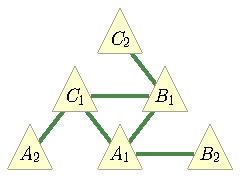
\includegraphics[scale=1]{injectiongraph222.pdf}
\caption{The auxiliary injection graph corresponding to the inflation DAG in \cref{fig:Tri222}, wherein a pair of nodes are adjacent iff they are pairwise injectable.}\label{fig:injection222}
\end{minipage}
%\hfill
%\begin{minipage}[b]{0.3\linewidth}
%\centering
%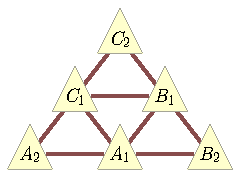
\includegraphics[scale=1]{ancestraldependancegraph222.pdf}
%\caption{An auxiliary ancestral dependance graph corresponding to the inflation DAG in \cref{fig:Tri222}, wherein a pair of nodes are adjacent iff they share a common ancestor.}\label{fig:dependances222}
%\end{minipage}
%\hfill
\hfill
\begin{minipage}[b]{0.5\linewidth}
\centering
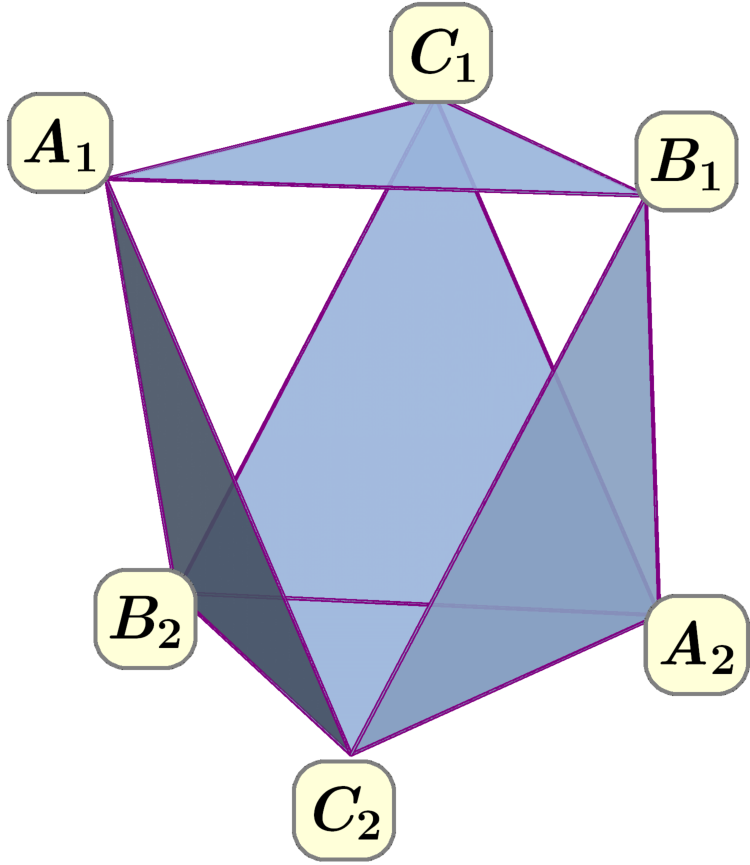
\includegraphics[scale=0.25]{simplicialcomplex.pdf}
\caption{The simplicial complex... \purp{Tobias - you please caption this?}The 5 faces in this figure correspond to the 5 maximal pre-injectable sets per \cref{fig:Tri222}, namely $\{A_1 B_1 C_1\}$, $\{A_1 B_2 C_2\}$, $\{A_2 B_1 C_2\}$, $\{A_2 B_2 C_1\}$ and $\{A_2 B_2 C_2\}$.}\label{fig:simplicialcomplex222}
\end{minipage}
\end{figure}

Applying these prescriptions to the inflation DAG in \cref{fig:Tri222} identifies 
 ancestral independencies and (pre-)injectable sets as follows:
\begin{align}\label{eq:basicsetup222}
{\underbrace{\begin{matrix}
A_2\aindep B_1\\
A_2\aindep C_2\\
B_2\aindep A_2\\
B_2\aindep C_1\\
C_2\aindep A_1\\
C_2\aindep B_2
\end{matrix}}_{\substack{\text{pairwise}\\\text{ancestral}\\\text{independencies}}}}
\qquad\quad
{\underbrace{\begin{matrix}
\\ \\
\brackets{A_2}\aindep \brackets{B_1 B_2 C_2}\\
\brackets{B_2}\aindep \brackets{A_2 C_1 C_2}\\
\brackets{C_2}\aindep \brackets{A_1 A_2 B_2}\\
\brackets{A_2}\aindep \brackets{B_2}\aindep \brackets{C_2}
\end{matrix}}_{\substack{\text{maximal}\\\text{ancestral}\\\text{independencies}}}}
\qquad\quad
{\underbrace{\begin{matrix}
\brackets{ A_1 B_1 }\\
\brackets{ B_1 C_1 }\\
\brackets{ A_1 C_1 }\\
\brackets{ A_2 C_1 }\\
\brackets{ B_2 A_1 }\\
\brackets{ C_2 B_1 }\\
\end{matrix}}_{\substack{\text{pairwise}\\\text{injectable}\\\text{sets}}}}
\qquad\quad
{\underbrace{\begin{array}{c}
\\ \\
\brackets{A_1 B_2}\\
\brackets{B_1 C_2}\\
\brackets{A_2 C_1}\\
\brackets{A_1 B_1 C_1}
\end{array}}_{\substack{\text{maximal}\\\text{injectable}\\\text{sets}}}}
\qquad\quad
{\underbrace{\begin{matrix}
\\
\brackets{A_1 B_1 C_1} \\
\brackets{A_1 B_2 C_2} \\
\brackets{A_2 B_1 C_2} \\
\brackets{A_2 B_2 C_1} \\
\brackets{A_2 B_2 C_2}
\end{matrix}}_{\substack{\text{maximal}\\\text{pre-injectable}\\\text{sets}}}}
\end{align}
such that the distributions on the pre-injectable sets relate to the original DAG distribution via
\begin{align}\label{eq:preinjectableuses222}
\begin{split}
&\forall_{a b c}:\; \begin{cases}
\pdf[A_1 B_1 C_1]{a b c} = \pdf[A B C]{a b c} \\
\pdf[A_1 B_2 C_2]{a b c} = \pdf[C]{c}\pdf[A B]{a b}\\%\pdf{C}\pdf{A B}\\
\pdf[A_2 B_1 C_2]{a b c} = \pdf[A]{a}\pdf[B C]{b c}\\
\pdf[A_2 B_2 C_1]{a b c} = \pdf[B]{b}\pdf[A C]{a c}\\
\pdf[A_2 B_2 C_2]{a b c} = \pdf[A]{a}\pdf[B]{b}\pdf[C]{c}
\end{cases}\end{split}
\end{align}
\cref{eq:preinjectableuses222} is an equivalent restatement of \cref{eq:tri222fac}. Having identified the pre-injectable sets (and how to use them), we next consider various ways to invoke constraints on the distributions over the pre-injectable sets.


\topic{\tred{Constraining Possible Distributions over Pre-Injectable Sets via the Marginal Problem}}\label{step:marginalsproblem}

The most trivial constraint on possible marginal probabilities, regardless of causal structure,  
%on the pre-injectable set
is simply the \emph{existence of some joint probability distribution} from which the marginal distributions can be recovered through marginalization, i.e. the possible marginal distributions must be \tblue{marginally compatible}. This isn't really causal inference -- as no hypothesis is considered -- but rather more of a preliminary sanity check. If the marginal distributions are not marginally compatible, then the answer to ``Can these marginal distributions be explained by this particular causal hypothesis?" is automatically ``No". 

The necessary and sufficient conditions for marginal compatibility are easy enough to state. There must exist some joint distribution (a collection of nonnegative joint probabilities) such that the marginal distributions can be recovered (each marginal distribution is a sum over various joint probabilities). \tblue{Solving the marginal problem} means resolving these "exists" statements into quantifier-free inequalities such that satisfaction of all such inequalities is necessary and sufficient for marginal compatibility. An efficient algorithm to solve the marginal problem is given in \cref{sec:projalgorithms}. The marginal problem comes up in a variety of applications, and has been studied extensively; see~\cite{fritz2013marginal} for further references.

As an example, here's how the marginal problem would be phrased as a partial-existential-closure problem with respect to the five three-variable marginal distributions corresponding to the pre-injectable sets in \cref{eq:preinjectableuses222}. For simplicity, we assume that all observable variables are binary\footnote{If the observables are not binary, then the resulting  binary-outcome inequalities are necessary for marginal compatibility, in that they should hold for any course-graining of the observational data into two classes, but the binary-outcome inequalities are no longer sufficient.}.

In order for the five pre-injectable sets in \cref{eq:preinjectableuses222} to be marginally compatible there must exist 64 nonnegative joint probabilities, i.e. satisfying
\begin{align}\label{eq:nonnegativity}
\forall_{a_1 a_2 b_1 b_2 c_1 c_2}:\;0\leq \pdf[A_1 A_2 B_1 B_2 C_1 C_2]{a_1 a_2 b_1 b_2 c_1 c_2},
\end{align}
constrained further by marginal distributions given by
\begin{align}\label[eqs]{eq:marginalequalities222}
\begin{split}
&\forall_{a_1 b_1 c_1}:\;\pdf[A_1 B_1 C_1]{a_1 b_1 c_1} = \sum\nolimits_{a_2 b_2 b_2}\pdf[A_1 A_2 B_1 B_2 C_1 C_2]{a_1 a_2 b_1 b_2 c_1 c_2},\\
&\forall_{a_1 b_2 c_2}:\;\pdf[A_2 B_2 C_2]{a_1 b_2 c_2} = \sum\nolimits_{a_2 b_1 c_1}\pdf[A_1 A_2 B_1 B_2 C_1 C_2]{a_1 a_2 b_1 b_2 c_1 c_2},\\
&\forall_{a_2 b_1 c_2}:\;\pdf[A_2 B_1 C_2]{a_2 b_1 c_2} = \sum\nolimits_{a_1 b_2 c_1}\pdf[A_1 A_2 B_1 B_2 C_1 C_2]{a_1 a_2 b_1 b_2 c_1 c_2},\\
&\forall_{a_2 b_2 c_1}:\;\pdf[A_2 B_2 C_1]{a_2 b_2 c_1} = \sum\nolimits_{a_1 b_1 c_2}\pdf[A_1 A_2 B_1 B_2 C_1 C_2]{a_1 a_2 b_1 b_2 c_1 c_2},\\
&\forall_{a_2 b_2 c_2}:\;\pdf[A_2 B_2 C_2]{a_2 b_2 c_2} = \sum\nolimits_{a_1 b_1 c_1}\pdf[A_1 A_2 B_1 B_2 C_1 C_2]{a_1 a_2 b_1 b_2 c_1 c_2}.
\end{split}
\end{align}
The marginal compatibility constraints in this case are, therefore, 64 inequalities and 40 equalities. Solving the marginal problem means eliminating 64 terms from those inequalities and equalities, namely any $\p[A_1 A_2 B_1 B_2 C_1 C_2]{\_\_\_\_\_\_}$. 
%We coin the term gedankenprobability to denote any probability pertaining to a \emph{not}-pre-injectable set of inflation-DAG variables. The gedankenprobabilities evoke thought experiments, because any \purp{black box implementation of the original causal structure % \emph{in-principle}.


Linear quantifier elimination is already widely used in causal inference to derive entropic inequalities \cite{fritz2013marginal,chaves2014novel,chaves2014informationinference}. In that task, however, the quantifiers being eliminated are those entropies which refer to hidden variables. By contrast, the probabilities we consider here are exclusively in terms of observable variables right from the very start. The quantifiers we eliminate are the not-pre-injectable joint probabilities, which are quite different from probabilities involving hidden variables.

When solving the marginal problem is too difficult, one may consider solving a relaxation of it, instead. One extremely computationally amenable relaxation of the marginal problem is to enumerate probabilistic Hardy-type paradoxes. This is discussed later on in  \cref{sec:TSEM}.

%\topic{\tred{Constraining Possible Distributions over Pre-Injectable Sets via Hardy Paradoxes}}

%Although solving the marginal problem can be highly optimized, it can still prove computationally difficult. It is therefore sometimes useful to consider relaxations of the marginals problem. The \emph{full} marginals problem is to find inequalities on the marginal distributions such that the inequalities are satisfied \emph{if and only if} the given marginal distributions can be extended. It is much easier to generate necessary-but-insufficient inequalities, i.e. satisfied by all compatible marginal distributions but such that no-violation does not certify marginal compatibility. We have identified a technique for rapidly generating such quantifier-free inequalities by restricting the search to inequalities of a very particular form. We found this alternative technique — trading generality for speed — to be extraordinarily practical. The type of inequalities that we consider are given by a certain class of tautologies in classical propositional logic, see \cref{sec:TSEM} for further details.

\topic{\tred{Constraining Possible Distributions over Pre-Injectable Sets via Conditional Independence Relations}}

The marginal problem asks about the existence of \emph{any} joint distribution which recovers the marginal distributions. In causal inference, however, there are plenty of other constraints on the sorts of joint distributions which are compatible with some causal hypothesis. The minimal constraint embedded in any causal hypothesis is the idea of causal structure. Thus it is natural to supplement the marginal problem with additional constraints, motivated by causal structure, on the hypothetical inflation-DAG observable joint distribution.

The most familiar causally-motivated constraints on a joint distribution are \tblue{conditional independence relations}, in particular, observable conditional independence relations. Conditional independence relations are inferred by $d$-separation; if $\bm{X}$ and $\bm{Y}$ are $d$-separated in the (inflation) DAG by $\bm{Z}$, then we infer the conditional independence $\bm{X}\bot\bm{Y}|\bm{Z}$. The $d$-separation criterion is explained at length in~\cite{pearl2009causality,studeny2005probabilistic,WoodSpekkens,pusey2014gdag}, so we elect not to review it here.

Every conditional independence relation can be translated into a nonlinear constraint on probabilities, as $\bm{X}\bot\bm{Y}|\bm{Z}$ implies $\p{\bm{x}\bm{y}|\bm{z}}=\p{\bm{x}|\bm{z}}\p{\bm{y}|\bm{z}}$ for all $\bm{x}$, $\bm{y}$, and $\bm{z}$. As we generally prefer to work with unconditional probabilities, we rewrite this as follows: If $\bm{X}$ and $\bm{Y}$ are $d$-separated by $\bm{Z}$, then $\p[\bm{X}\bm{Y}\bm{Z}]{\bm{x}\bm{y}\bm{z}}\p[\bm{Z}]{\bm{z}}=\p[\bm{X}\bm{Z}]{\bm{x}\bm{z}}\p[\bm{Y}\bm{Z}]{\bm{y}\bm{z}}$ for all $\bm{x}$, $\bm{y}$, and $\bm{z}$. Such nonlinear constraints can be incorporated as further restrictions on the sorts of joint distributions compatible with the inflation DAG, supplementing the basic nonnegativity of probability constraints of the marginal problem. 

For example, in \cref{fig:Tri222} we find that $A_1$ and $C_2$ are $d$-separated by $\{A_2 B_2\}$, and so one might incorporate the family of nonlinear equalities $\p[A_1 A_2 B_2 C_2]{a_1 a_2 b_2 c_2}\p[A_2 B_2]{a_2 b_2}=\p[A_1 A_2 B_2]{a_1 a_2 b_2}\p[A_2 B_2 C_2]{a_2 b_2 c_2}$ for all $a_1$, $a_2$, $b_2$ and $c_2$. Note that every semi-marginal probability introduced in some nonlinear condition independence equation should also be \emph{defined} by marginalization, i.e. as a sum of various joint probabilities, so that one need not eliminate further quantifiers. The relevant substitutions of this example would be
\begin{align}
\begin{array}{lll}
\forall_{a_2 b_2}:&\;\pdf[A_2 B_2]{a_2 b_2} \to& \sum\nolimits_{a_1 b_1 c_1 c_2}\pdf[A_1 A_2 B_1 B_2 C_1 C_2]{a_1 a_2 b_1 b_2 c_1 c_2},\\
\forall_{a_1 a_2 b_2 c_2}:&\;\pdf[A_1 A_2 B_2 C_2]{a_1 a_2 b_2 c_2} \to& \sum\nolimits_{b_1 c_1}\pdf[A_1 A_2 B_1 B_2 C_1 C_2]{a_1 a_2 b_1 b_2 c_1 c_2},\\
\forall_{a_1 a_2 b_2}:&\;\pdf[A_1 A_2 B_2]{a_1 a_2 b_2} \to\quad& \sum\nolimits_{b_1 c_1 c_2}\pdf[A_1 A_2 B_1 B_2 C_1 C_2]{a_1 a_2 b_1 b_2 c_1 c_2}
\end{array}
\end{align}
etc. 
%Note also that incorporating such constraints also increases the number of quantifier which must be eliminated, as additional non-injectable probabilities are now featured in the equalities corresponding to conditional independence which do not appear in the unconstrained marginal problem. 

Many modern computer algebra systems have functions capable of tackling nonlinear quantifier elimination symbolically\footnote{For example \textit{Mathematica$^{_{\textit{\tiny\texttrademark}}}$}'s \href[pdfnewwindow]{http://reference.wolfram.com/language/ref/Resolve.html}{\texttt{Resolve}} command, \textit{Redlog}'s \href[pdfnewwindow]{http://www.redlog.eu/documentation/reals/rlqe.php}{\texttt{rlposqe}}, or \textit{Maple$^{_{\textit{\tiny\texttrademark}}}$}'s \href[pdfnewwindow]{http://maplesoft.com/support/help/Maple/view.aspx?path=RegularChains/SemiAlgebraicSetTools/RepresentingQuantifierFreeFormula}{\texttt{RepresentingQuantifierFreeFormula}}, etc.}. 
%One might then hope to use such software systems to rid the hybrid inequalities of the gedankenprobabilities. 
Currently, however, it is not practical to perform nonlinear quantifier elimination on large polynomial systems with many quantifiers. It may be possible to exploit results on the particular algebraic-geometric structure of these particular systems~\cite{garcia_bayesian_2005}. But also without using quantifier elimination, the nonlinear constraints can be easily accounted for numerically. Upon substituting numerical values for all the injectable probabilities, the former quantifier elimination problem is converted to a universal quantifier existence problem: Do there exist quantifier that satisfy the full set of linear and nonlinear numeric (as opposed to symbolic) constraints? Most computer algebra systems can resolve such \emph{satisfiability} questions quite rapidly\footnote{For example \textit{Mathematica$^{_{\textit{\tiny\texttrademark}}}$} \href[pdfnewwindow]{http://reference.wolfram.com/language/Experimental/ref/ExistsRealQ.html}{\texttt{Reduce\`{}ExistsRealQ}} function. Specialized satisfiability software such as SMT-LIB's \href[pdfnewwindow]{http://smtlib.cs.uiowa.edu/solvers.shtml}{\texttt{check-sat}} \cite{BarFT-SMTLIB} are particularly apt for this purpose.
%One can also exploit the fact than any nonlinear optimizer will return an error when a set of constraints cannot be satisfied. Nonlinear optimizers include \textit{Maple$^{_{\textit{\tiny\texttrademark}}}$}'s \href[pdfnewwindow]{http://www.maplesoft.com/support/help/Maple/view.aspx?path=Optimization/NLPSolveMatrixForm}{\texttt{NLPSolve}}, \textit{Mathematica$^{_{\textit{\tiny\texttrademark}}}$}'s \href[pdfnewwindow]{http://reference.wolfram.com/language/ref/message/NMinimize/nsol.html}{\texttt{NMinimize}}, and dozens of free and commercial optimizers for \href[pdfnewwindow]{http://ampl.com/products/solvers/all-solvers-for-ampl}{\textit{AMPL}} and/or \href[pdfnewwindow]{https://neos-server.org/neos/solvers/index.html\#nco}{\textit{GAMS}}
}.


It is also possible to use a mixed strategy of linear and nonlinear quantifier elimination, such as \citet{ChavesPolynomial} advocates. The explicit results of Ref. \cite{ChavesPolynomial} are therefore consequences of any inflation DAG, achieved by applying a mixed quantifier elimination strategy.

\topic{\tred{Constraining Possible Distributions over Pre-Injectable Sets via Coinciding Marginals}}

The inflation hypothesis is more than just causal structure, however, even if the original hypothesis did not constrain possible causal models beyond the original DAG.  By restricting to exclusively \emph{inflation} models, however, we require $\pdf{A_i| \Pa[G']{A_i}}=\pdf{A_j|\Pa[G']{A_j}}$, per \cref{eq:funcdependences}. Consequently, the distributions over different injectable sets must occasionally coincide, i.e. $\pdf{\bm{X}}=\pdf{\bm{Y}}$ whenever both $\bm{X}$ and $\bm{Y}$ are injectable, and $\subsim{\bm{X}}=\subsim{\bm{Y}}$. Sometimes sets of random variables which are \emph{not} injectable, however, can also be shown to have necessarily coinciding distributions. For example, we can verify that $\pdf{A_1 A_2 B_1}=\pdf{A_1 A_2 B_2}$ follows from \cref{fig:Tri222}, even though $\brackets{A_1 A_2 B_1}$ and $\brackets{A_1 A_2 B_2}$ are not injectable sets.

Equations such as $\forall_{a_1 a_2 b}:\;\p[A_1 A_2 B_1]{a_1 a_2 b} = \p[A_1 A_2 B_2]{a_1 a_2 b}$ are also intrinsic parts of the inflation hypothesis, and may incorporated into either linear or nonlinear quantifier eliminations in order to derive stronger incompatability witnesses. The details of how to recognize coinciding distributions beyond the obvious coincidences implied by injectable or pre-injectable sets are discuss in \cref{sec:coincidingdetails}.



%One may also substitute numeric values for all the pre-injectable probabilities appearing in the marginals problem. Upon doing so, the quantifier elimination problem is converted to a quantifier existence problem: Do there exist gedankenprobabilities that satisfy the resulting system of inequalities? Such \emph{satisfiability} questions can be resolved quite rapidly, especially when the quantifiers are linear \cite{Korovin2012ImplementingCRA,Bobot2012SimplexSAT}. Note that real-world data with uncertainties can also be incorporated into these satisfiability questions. Instead of asserting that a particular probability is equal to a given \emph{value}, one can incorporate new inequalities which constrain the experimentally-known probabilities to lie in given \emph{intervals}. Assigning probabilities to intervals as opposed to numeric values results in further free parameters in the system, but the problem nevertheless remains one of \emph{universal} existential closure, and can be resolved with extreme efficiency.


%One useful alternative to linear quantifier elimination is to identify representative probability distributions which are incompatible with the (unprojected) constraints; \citet{ChavesNoSignalling} use this technique, for example. %That technique essentially translates the elimination problem to a satisfiability problem, and moreover an ultra-efficient \emph{linear} quantifier existence problem at that! In the context of polytope projection, these representative probability distributions correspond to extreme rays of the so-called ``projection cone" \cite{jones2004equality,Jones2008,BalasProjectionCone}.

%A final alternative to linear quantifier elimination is to restrict one's consideration to quantifier-free inequalities with a particular form. We found this alternative technique — trading generality for speed — to be extraordinarily practical. The subtype of causal criteria which can be most rapidly recognized are those which follow from certain tautologies in classical propositional logic, see \cref{sec:TSEM} for further details.




%\purp{It is interesting to compare the technique for deriving polynomial inequalities here to that in in Ref. \cite{ChavesPolynomial}. One the one hand, our initial set of linear inequalities is much stronger, as we work with the inflated DAG whereas \citet{ChavesPolynomial} considers only the original DAG. This allows us to analyze scenarios which Ref. \cite{ChavesPolynomial} cannot, namely those without any observable conditional independence relations, such as the Triangle scenario. On the other hand, Ref. \cite{ChavesPolynomial} purportedly incorporates any kind of observable conditional independence relation, whereas we account only for \emph{unconditional} independence relations, per \cref{step:fac}. A careful examination of Ref. \cite{ChavesPolynomial}, however, reveals that only unconditional independence relations are utilized in all the example there. To that extent, therefore, all the explicit results in Ref. \cite{ChavesPolynomial} are implied by the inflation DAG technique.}

%We note that our polynomial inequalities are related to those introduced recently by \citet{ChavesPolynomial}, in that our inequalities subsume the explicit results of Ref. \cite{ChavesPolynomial}. \purp{NEEDS CONFIRMATION!} \citet{ChavesPolynomial} exploits conditional independence at the observable level only, whereas our technique is applicable to scenarios even without any observable CI relations, such as the Triangle scenario.

\purp{Move this paragraph up, Tobias? ~EW}
As far as we can tell, our inequalities are not related to the nonlinear incompatability witnesses which have been derived specifically to constrain classical networks \cite{TavakoliStarNetworks,RossetNetworks,TavakoliNoncyclicNetworks}, nor to the nonlinear inequalities which account for interventions to a given causal structure \cite{kang2007polynomialconstraints,steeg2011relaxation}.




\section{Bell scenarios and inflation}
\label{sec:Bellscenarios}

\begin{comment}


\begin{figure}[b]
\centering
\begin{minipage}[t]{0.45\linewidth}
\centering
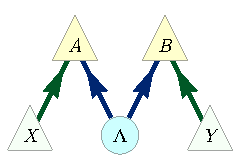
\includegraphics[scale=1]{BellDagRaw.pdf}
\caption{The causal structure of the a bipartite Bell scenario. The local outcomes of Alice's and Bob's experimental probing is assumed to be a function of some latent common cause, in addition to their independent local experimental settings.}\label{fig:NewBellDAG}
\end{minipage}
\hfill
\begin{minipage}[t]{0.45\linewidth}
\centering
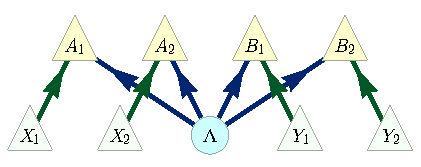
\includegraphics[scale=1]{BellDagCopy.pdf}
\caption{An inflation DAG of the bipartite Bell scenario, where both local settings variables have been duplicated.}\label{fig:BellDagCopy}
\end{minipage}
\end{figure}
\end{comment}

To further illustrate our inflation-DAG approach, we demonstrate how to recover all Bell inequalities \cite{Brunner2013Bell,bell1966lhvm,CHSHOriginal} via our method. To keep things simple we only discuss the case of a bipartite Bell scenario with two possible ``settings'' here, but the cases of more settings and/or more parties are totally analogous.
%It is critical that our method should be able to derive these seminal criteria, as Bell inequalities have been a foundational component of quantum information theory for the last half century \cite{scarani2012device,BancalDIApproach}.

Consider the causal structure associated to the Bell/CHSH \cite{bell1964einstein,Brunner2013Bell,bell1966lhvm,CHSHOriginal} experiment [\citealp{pusey2014gdag}~(Fig.~E\#2), \citealp{WoodSpekkens}~(Fig.~19), \citealp{chaves2014novel}~(Fig.~1), \citealp{BeyondBellII}~(Fig.~1), \citealp{wolfe2015nonconvexity}~(Fig.~2b), \citealp{steeg2011relaxation}~(Fig.~2)], depicted here in \cref{fig:NewBellDAG1}. The observable variables are $A,B,X,Y$, and $\Lambda$ is the latent common cause of $A$ and $B$.

In the Bell scenario DAG, one usually works with the conditional distribution $P(AB|XY)$ instead of with the original distribution $P(ABXY)$. The conditional distribution is an \emph{array} of distributions over $A$ and $B$, indexed by the possible values of $X$ and $Y$. The maximal pre-injectable sets then are
\begin{align}\begin{split}
&\brackets{A_1 B_1, X_1 X_2 Y_1 Y_2} \\
&\brackets{A_1 B_2, X_1 X_2 Y_2 Y_2} \\
&\brackets{A_2 B_1, X_1 X_2 Y_2 Y_2} \\
&\brackets{A_2 B_2, X_1 X_2 Y_2 Y_2} ,
\end{split}\end{align}
where we have put commas in order to clarify that every maximal pre-injectable set contains \emph{all} ``settings'' variables. These pre-injectable sets are specified by the original observable distribution via
\begin{align}\begin{split}&\forall_{a b x_1 x_2 y_1 y_2}:\; \begin{cases}
	P_{A_1 B_1 X_1 X_2 Y_1 Y_2}(a b x_1 x_2 y_1 y_2)  = P_{A B X Y}(a b x_1 y_1) P_X(x_2) P_Y(y_2), \\
	P_{A_1 B_2 X_1 X_2 Y_1 Y_2}(a b x_1 x_2 y_1 y_2)  = P_{A B X Y}(a b x_1 y_2) P_X(x_2) P_Y(y_1), \\
	P_{A_2 B_1 X_1 X_2 Y_1 Y_2}(a b x_1 x_2 y_1 y_2)  = P_{A B X Y}(a b x_2 y_1) P_X(x_1) P_Y(y_2), \\
	P_{A_2 B_2 X_1 X_2 Y_1 Y_2}(a b x_1 x_2 y_1 y_2)  = P_{A B X Y}(a b x_2 y_2) P_X(x_1) P_Y(y_1), \\
		P_{X_1 X_2 Y_1 Y_2}(x_1 x_2 y_1 y_2)  = P_X(x_1) P_X(x_2) P_Y(y_1) P_Y(y_2).
\end{cases}\end{split}\end{align}
%where it should be understood implicitly that the inequalities hold for all values of $\{a b x_1 x_2 y_1 y_2\}$.
%The last equations follows from each of the others by making use of the Markov condition $P_{XY} = P_X P_Y$ for the original distribution, it nevertheless
By dividing the first four inequalities by the latter we obtain
\begin{align}\begin{split}\forall_{a b x_1 x_2 y_1 y_2}:\; \begin{cases}
	P_{A_1 B_1 | X_1 X_2 Y_1 Y_2}(a b | x_1 x_2 y_1 y_2)  = P_{A B | X Y}(a b | x_1 y_1) \\
	P_{A_1 B_2 | X_1 X_2 Y_1 Y_2}(a b | x_1 x_2 y_1 y_2)  = P_{A B | X Y}(a b | x_1 y_2) \\
	P_{A_2 B_1 | X_1 X_2 Y_1 Y_2}(a b | x_1 x_2 y_1 y_2)  = P_{A B | X Y}(a b | x_2 y_1) \\
	P_{A_2 B_2 | X_1 X_2 Y_1 Y_2}(a b | x_1 x_2 y_1 y_2)  = P_{A B | X Y}(a b | x_2 y_2).
\end{cases}\end{split}\end{align}
If we then impose marginal compatibility according the the marginal problem we find that the (minimal!) consequence of the inflation hypothesis is 
\begin{align}
	P_{A_1 B_1 | X_1 X_2 Y_1 Y_2}(a b | x_1 x_2 y_1 y_2)  =  \sum\nolimits_{a_2,b_2} P_{A_1 A_2 B_1 B_2 X_1 X_2 Y_1 Y_2}(a_1 a_2 b_1 b_2|x_1 x_2 y_1 y_2)
\end{align}
etc.
For the inflated observation data to compatible with the inflation hypothesis, therefore, we would require
\begin{align}\begin{split}\label{eq:finalBellstep}\forall_{a b}:\; \begin{cases}
	P_{A B | X Y}(a b | 0 0)  =  \sum\nolimits_{a',b'} P_{A_1 A_2 B_1 B_2 X_1 X_2 Y_1 Y_2}(a a' b b'|0101) \\
	P_{A B | X Y}(a b | 1 0)  =  \sum\nolimits_{a',b'} P_{A_1 A_2 B_1 B_2 X_1 X_2 Y_1 Y_2}(a' a b b'|0101) \\
	P_{A B | X Y}(a b | 0 1)  =  \sum\nolimits_{a',b'} P_{A_1 A_2 B_1 B_2 X_1 X_2 Y_1 Y_2}(a a' b' b|0101) \\
	P_{A B | X Y}(a b | 1 1)  =  \sum\nolimits_{a',b'} P_{A_1 A_2 B_1 B_2 X_1 X_2 Y_1 Y_2}(a' a b' b|0101)
\end{cases}\end{split}\end{align}
The existence of an \emph{array} of distributions, i.e. \cref{eq:finalBellstep}, is equivalent to the existence of a \tblue{hidden variable model}, as noted in Fine's Theorem~\cite{FineTheorem}. Thus, an inflation model exists if and only if a hidden-variable model exists for the original observable variables.

%The last equations turns out to be rather useful to write down explicitly: putting $x_1 = y_1 = 0$ and $x_2 = y_2 = 1$ and dividing the first equation by the last one results in
%\begin{align*}
%	P_{A B X Y}(a b | 0 0)  =  \sum_{a',b'} P_{A_1 A_2 B_1 B_2 X_1 X_2 Y_1 Y_2}(aa'bb'|0101).
%\end{align*}
%Similarly, $P_{A B X Y}(a b | 0 1)$, $P_{A B X Y}(a b | 1 0)$ and $P_{A B X Y}(a b | 1 1)$ can also be written as marginals of a conditional distribution. 
%By Fine's Theorem~\cite{FineTheorem}, this implies the existence of a hidden-variable model. Conversely, if a hidden-variable model exists, then the existence of the inflation model implies the existence of a solution to the marginal problem.

In conclusion, we therefore find in the case of the inflation DAG~\cref{fig:BellDagCopy1}, the inflation method yields \emph{tight} incompatability witnesses for the Bell causal structure, i.e. the Bell/CHSH inequalities, just by requiring marginal compatibility of the pre-injectable sets.
More generally, we can use Fine's theorem to show that applying the marginal problem to suitable inflation DAGs can reproduce \emph{all} Bell inequalities, for any standard Bell scenario, no matter how many parties or settings or possible outcomes. 

\begin{comment}
Analysis of the inflated DAG in \cref{fig:BellDagCopy1} shows that 
\begin{align}\label{eq:bellypolymapped}
 \p{a b x y}\p{\n{x}} \p{\n{y}}
&\leq
 \p{a \n{b} x \n{y}}\p{\n{x}}\p{y} +  \p{\n{a} b \n{x} y}\p{x} \p{\n{y}}+\p{a b \n{x} \n{y}}\p{x} \p{y}
\\
\shortintertext{by virtue of the unmapped (but factored) inequality}
\label{eq:bellypolyunmapped}
 \p{a_1 b_1 x_1 y_1}\p{\n{x}_2} \p{\n{y}_2}
&\leq
 \p{a_1 \n{b}_2 x_1 \n{y}_2}\p{\n{x}_2} \p{y_1} +\p{\n{a}_2 b_1 \n{x}_2 y_1}\p{x_1}\p{\n{y}_2}+  \p{a_2 b_2 \n{x}_2 \n{y}_2}\p{x_1} \p{y_1}
\end{align}
where \emph{every} probability appearing in \cref{eq:bellypolyunmapped} maps to the original scenario, hence yielding \cref{eq:bellypolymapped}. To derive the usual Bell inequalities from \cref{eq:bellypolymapped} we switch to conditional probabilities via ${\p{a b x y}\to\p{a b | x y}\p{x y}=\p{a b | x y}\p{x}\p{y}}$ which, after dividing both sides of \cref{eq:bellypolymapped} by $\p{x}\p{\n{x}}\p{y}\p{\n{y}}$, yields
\begin{align}\label{eq:chwithneg}
&\p{a b | x y}
\leq
{\p{a \n{b} | x \n{y}} + \p{\n{a} b | \n{x} y}+\p{a b | \n{x} \n{y}}}
\\
\hspace{-\mathindent}\text{or, equivalently,}\quad
\label{eq:chwithoutneg}
&{\p{a b | x y}+\p{a b | x \n{y}} + \p{a b | \n{x} y}}
\leq
{\p{a|\n{x}}+\p{b|\n{y}} + \p{a b | \n{x} \n{y}}}
\end{align}
which is precisely the Clauser-Horne (CH) inequality \cite{CHInequality} for the Bell scenario. Note that to obtain \cref{eq:chwithoutneg} from \cref{eq:chwithneg} we implicitly made use of the no-signalling assumptions, namely $\p{a|x y}=\p{a|x}$ and $\p{b| x y}=\p{b | y}$. The CH inequality is the \emph{unique} Bell inequality (up to permutations) for the Bell scenario if $\brackets{A,B,X,Y}$ are all binary, and hence the CH inequality is a necessary and sufficient criterion to ascertain if correlations are compatible with that Bell scenario variant.

The causal structure of a Bell scenario can also be formulated directly in terms of conditional random variables. For example, the conditional-structure interpretation of \cref{fig:BellDagCopy1} is \cref{fig:BellConditionalDAG}. 

\begin{figure}[t]
\centering
\begin{minipage}[t]{0.45\linewidth}
\centering
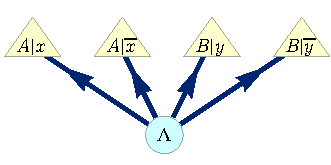
\includegraphics[scale=1]{BellDagConditionForm.pdf}
\caption{The causal structure of the Bell scenario expressed in a form which makes use of conditional random variables.}\label{fig:BellConditionalDAG}
\end{minipage}
%\hfill
%\begin{minipage}[t]{0.45\linewidth}
%\centering
%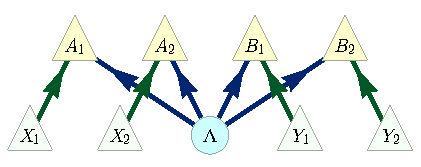
\includegraphics[scale=1]{BellDagCopy.pdf}
%\caption{An inflation DAG of the Bell scenario, where both local settings variables have been duplicated.}\label{fig:BellDagCopy}
%\end{minipage}
\end{figure}

The Bell inequalities are then self-evident from \cref{fig:BellConditionalDAG} without the need for an inflation DAG. The conditional-structure formulation innately implies its own inaccessible gedankenprobabilities, such as $\{\p{a|x , a|\n{x}}$, $\p{a|x , \n{a}|\n{x}},...\}$ etc. By eliminating these gedankenprobabilities from the set of inequalities generated by $0\leq \pdf{A|x , A|\n{x} , B|y , B|\n{y}}$ we obtain
\begin{align}\label{eq:bellcondeq}
0
\leq
{\p{a|\n{x}} + \p{b|\n{y}} + \p{a|x , b|y} -\p{a|x ,b|\n{y}} -\p{a|\n{x} , b|y} -\p{a|\n{x} , b|\n{y}}}\,,
\end{align}
for example. It should be clear that \cref{eq:bellcondeq} is equivalent to \cref{eq:chwithoutneg}.

%We can perform quantifier elimination on the set of (polynomial) inequalities given by $0\leq \pdf{A|x , A|\n{x} , B|y , B|\n{y}}$. The use of a conditional-structure DAG innately implies certain inaccessible gedankenprobabilities, such as $\{\p{a|x , a|\n{x}}$, $\p{a|x , \n{a}|\n{x}},...\}$ etc. 
\purp{Rob says kill next two paragraphs?}

Conditional-structure gedankenprobabilities are somewhat different from the inflation DAG kind, in that they reference multiple counterfactual events, such as ``What is the probability that Alice would choose to visit the museum \emph{IF} (given that) it's a rainy day in Maryland \emph{AND} that Alice would choose to go the beach \emph{IF} (given that) it's sunny in Maryland?". By contrast, unconditional gedankenprobabilities which live on an inflation DAG reference multiple heterofactual (for lack of a better word) events, such as ``What is the probability that Alice-copy-\#1 chooses to visit the museum \emph{AND} that it's raining in Maryland-copy-\#1 \emph{AND} that Alice-copy-\#2 chooses to go the beach \emph{AND} that it's sunny in Maryland-copy-\#2?". 

Joint counterfactual probabilities are experimentally inaccessible, just the same as joint heterofactual probabilities are. Suppose one could establish both Alice's propensity for going to the museum when it rains and her propensity for going to the beach when it's sunny. Even so, neither the joint counterfactual probability nor the joint heterofactual probability can be established from that limited data. For example, the value of the hidden variable ${\Lambda\cramp{=}\lambda}$ may influence Alice's willingness to get out of bed at all, or determine if she is on-call as a volunteer EMT on a particular day, or $\lambda$ might encode if Alice is travelling out-of-state. If we could measure $\p{a|x , \n{a}|\n{x}},...\}$ we might learn that Alice's likelihood of visiting the museum if it rains in Maryland is highly correlated with her likelihood of visiting the beach when it's sunny in Maryland. Or we might learn that those two counterfactual probabilities are relatively statistically independent. The ``hidden-ness" of the classical variable corresponding to the latent node shields the gedankenprobabilities from being determined. 
\end{comment}

\section{Quantum Causal Inference and the No-Broadcasting Theorem}\label{sec:classicallity}

In the causal inference problems with latent nodes that we have considered so far, the latent nodes correspond to unobserved random variables. This describes things that come up in \emph{classical} physics (and things outside of physics). In \emph{quantum} physics, however, the latent nodes may instead carry \emph{quantum systems}. Whenever this is allowed, we say that the DAG represents a \tblue{quantum causal structure}. Some quantum causal structures are famously capable of generating distributions over the observable variables that would not be possible classically.

The set of quantumly realizable distributions is superficially quite similar to the classical subset \cite{pusey2014gdag,fritz2012bell}. For example, classical and quantum distributions alike respect all conditional independence relations implied by the common underlying causal structure \cite{pusey2014gdag}. It is an interesting problem to find quantum distributions that are not realizable classically, or to show that there are no such distributions on a given DAG.

However, this is by no means an easy task. For example, recent work has found that quantum causal structure also implies many of the entropic inequalities that hold classically~\cite{pusey2014gdag,Chaves2015infoquantum,ChavesNoSignalling}. To date, no quantum distribution has been found to violate a Shannon-type entropic inequality on observable variables derived from the Markov conditions on all nodes \cite{chaves2012entropic,fritz2012bell}. Fine-graining the scenario by conditioning on root variables (``settings'') leads to a different kind of entropic inequality, and these have proven somewhat quantum-sensitive \cite{braunstein1988entropic,SchumacherInequality,chaves2014novel}. Such inequalities are still limited, however, in that they only apply in the presence of observable root nodes\footnote{Rafael Chaves and E.W. are exploring the potential of entropic analysis based on conditioning on non-root observable nodes. This generalizes the method of entropic inequalities, and might be capable of providing much stronger entropic witnesses.}, and they still fail to witness certain distributions as classically infeasible~\cite{chaves2014novel,fritz2012bell}.

We hope that polynomial inequalities derived from broadcasting inflation DAGs will provide an additional tool for witnessing certain quantum distributions as non-classical. For example due to the results of~\cref{sec:Bellscenarios}, it seems conceivable that these inequalities will be much stronger and provide much tighter constraints than entropic inequalities.

It is worth pondering how it is possible that some of the inequalities that can be derived via inflation---such as Bell inequalities---have quantum violations, i.e.~why one cannot expect them to be valid for all quantum distributions as well. The reason for this is that duplicating an outgoing edge in a DAG during inflation amounts to \tblue{broadcasting} the value of the random variable. For example while the information about $X$ in~\cref{fig:TriMainDAG} was ``sent'' to $A$ and $C$, the information about $X_1$ is sent to $A_1$ \emph{and} $A_2$ and $C$ in the inflation \cref{fig:simpleinflation}. Since quantum theory satisfies a no-broadcasting theorem~\cite{NoCloningQuantum1996,NoCloningGeneral2006}, one cannot expect such broadcasting to be possible quantumly. More generally, there is an analogous no-broadcasting theorem in the regime of epistemically restricted general probabilistic theories (GPTs) \cite{SpekkensToyTheory,NoCloningGeneral2006,Barnum2012GPT,Janotta2014GPT}, so that the same statement applies in many theories other than quantum theory. As a consequence, a quantum or general probabilistic causal model on the original DAG does generally not inflate to a ``quantum inflation model'' or ``general probabilistic inflation model'' on the inflation DAG. 

Some inflations, such as the one of~\cref{fig:TriDagSubA2B1C1}, do not require such broadcasting.

\begin{definition}
	$G'\in\SmallNamedFunction{Inflations}{G}$ is \tblue{non-broadcasting} if every latent node in $G'$ has at most one copy of each $A\in\SmallNamedFunction{Nodes}{G}$ among its children.
\end{definition}

It follows that every quantum causal model can be inflated to a non-broadcasting DAG, so that one obtains a quantum and general probabilistic analogue of Lemma~\ref{mainlemma} in the non-broadcasting case. Constraints derived from non-broadcasting inflations are therefore valid also for quantum and even general probabilistic distributions. In the specific case of the entropic monogamy inequality for the Triangle scenario, i.e. \cref{eq:monogomyofcorrelations} here, this was originally noticed in Ref.~\cite{pusey2014gdag}. Another example is \cref{eq:polymonogamy}, which was derived from the non-broadcasting inflation of \cref{fig:TriDagSubA2B1C1}. \cref{eq:polymonogamy} too, therefore, is a necessary criterion for compatibility with the Triangle scenario even when the latent nodes are allowed to carry quantum or general probabilistic systems.
% This confirms our numerical computations, which indicated that~\eqref{eq:polymonogamy} does not have any quantum violations. The same is true for monogamy of correlations, per \cref{eq:monogomyofcorrelations}.
Since the perfect-correlation distribution considered in~\cref{eq:ghzdistribution1} violates both of these inequalities, it evidently cannot be generated within the Triangle scenario even with quantum or general probabilistic states on the hidden nodes. This was also pointed out in Ref.~\cite{pusey2014gdag}.

%\begin{align}\label{eq:nonbroadcastinginflationDAG}
%G'\in\SmallNamedFunction{NonBroadcastingInflations}{G} \quad\text{ iff }\quad \forall_{\text{latent }A_i\in G'}\; \Ch[G']{A_i} \text{ is an irredundant set.}
%\end{align}

On the other hand, by intentionally using broadcasting in an inflation DAG, we can specifically try to witness certain quantum or general probabilistic distributions as non-classical. This is exactly what happens in Bell's theorem.

%  We also find it useful to define the notion of a non-broadcasting subset of nodes within some larger broadcasting inflation DAG.
% Let's define any pair of redundant nodes which share a latent parent to be a \tblue{fundamental broadcasting pair}. An inflation DAG is non-broadcasting if it does not contain any fundamental broadcasting pairs. Similarly, a set of nodes $\bm{U}$ is a \tblue{non-broadcasting set} iff $\An[G']{\bm{U}}$ is free of any fundamental broadcasting pairs.

%A set of nodes $\bm{U}$ is a \tblue{non-broadcasting set} iff $\ansubgraph[G']{\bm{U}}$ is a non-broadcasting inflation DAG. Any inference about the original DAG which can be made by referencing exclusively to non-broadcasting sets hold in both the classical and quantum paradigms. Broadcasting inflation DAGs are therefore especially useful for deriving criteria which distinguish quantum and classical probability distributions, but we anticipate them to be valuable for broader causal inference tasks as well.

% It is worth emphasizing that broadcasting the values of hidden variables %which are predicated on multiple counterfactual or heterofactual events 
%are strictly classical constructs. If the latent node in the Bell scenario in \cref{fig:NewBellDAG1} is allowed to be a quantum resource $\mathcal{H}^{d_A\otimes d_B}$, for example, then broadcasting gedankendistributions such as $\pdf{A|x , A|\n{x},...}$ or $\pdf{A_1,A_2,...}$ are \tblue{physically prohibited} if the quantum state is suitably entangled.

% More precisely, quantum states are governed by a no-broadcasting theorem \cite{NoCloningQuantum1996,NoCloningGeneral2006}: If half the state is sent to Alice and she performs some measurement on it, she fundamentally perturbs the state by measuring it. Post-measurement, that half of the state cannot be ``re-sent" to Alice, that she might re-measure it using a different measurement setting. As a consequence of the no-broadcasting theorem, in the inflation DAG picture a quantum state which was initially available to a single party cannot be distributed both to Alice-copy-\#1 and Alice-copy-\#2 in the way a classical hidden variable could be. 

% This means that considerations on inflation DAGs cannot be used to derive quantum causal infeasibility criteria whenever a gedankenprobability presupposes the ability to broadcast a latent node's system. Broadcasting and non-broadcasting sets of variables are distinguished per \cref{eq:nonbroadcastinginflationDAG}.

%When analyzing GPT causal structures one may not assume that a joint probability distribution over observable variables is universally nonnegative if the set of observable variables has simultaneous meaning only under broadcasting of latent variables. This is in direct contrast to \cref{step:generateineqs} in \cref{sec:mainalgorithm}. 

%Not every inflation requires broadcasting, however, and hence not every gedankenprobability is physically prohibited by quantum theory. 
%An inflation DAG is a \tblue{non-broadcasting inflation} whenever the children of every individual node in the inflation DAG $G'$ map injectively to the corresponding children of the mapped node in the original DAG $G$, i.e. $dmap\parenths*{\Ch[G']{X}}\subseteq\Ch[G]{dmap\parenths*{X}}$ for all $X\in\nodes{G'}$. 
% \cref{fig:TriDagSubA2B1C1} is an example of a non-broadcasting inflation.

Even when using broadcasting inflation DAGs, it may still be possible to derive inequalities valid for quantum distributions if one appropriately the nonnegativity inequalities in the marginal problem, e.g. such as \cref{eq:nonnegativity}. The modification would replace demanding nonnegativity of the full joint distribution with instead demanding the nonnegativity of only quantum-physically-meaningful marginal probability distributions. 

Even when using broadcasting inflation DAGs, it may still be possible to derive inequalities valid for quantum distributions if one appropriately modifies \cref{sec:ineqs} to generate a different initial set of nonnegativity inequalities. This new set should capture the nonnegativity of only quantum-physically-meaningful marginal probability distributions. Indeed, a quantum causal model on the original DAG can potentially be inflated to a quantum inflation model on the inflation DAG in terms of the logical broadcasting maps of \citet{Coecke2011}. From this perspective, a broadcasting inflation DAG is an abstract logical concept, as opposed to a feasible physical construct. However, this would result in a joint distribution over all observable variables that may have some negative probabilities, and one cannot expect~\cref{eq:nonnegativity} to hold in general. But one can still try to reformulate the marginal problem so as to refer only to the existence of joint distributions on non-broadcastings sets rather than the existence of a full joint distribution from which the marginal distributions might be recovered. Here, a set $\bm{U}$ of observable nodes is non-broadcasting if $\An{\bm{U}}$ does not two distinct copies of a node which have a parent in common.

An analysis along these lines has already been carried out successfully by \citet{Chaves2015infoquantum} in the derivation of entropic inequalities that are valid for all quantum distributions. Although \citet{Chaves2015infoquantum} do not invoke inflation DAGs, they do seem to employ a similar type of structure to model the conditioning of a variable on a ``setting'' variable, and this also gives rise to non-broadcasting sets. \citet{Chaves2015infoquantum} take pains to avoid including full joint probability distributions in any of their initial entropic inequalities, precisely as we would want to do in constructing our initial probability inequalities, and they successfully derive quantumly valid entropic inequalities. But so far, no inequalities polynomial in the probabilities have been derived using this method.

% Our current inflation DAG method can be employed to derive causal infeasibility criteria for general causal structures, thus generalizing Bell inequalities somewhat. From a quantum foundations perspective, however, generalizing Tsirelson inequalities \cite{Tsirelson1980,Brunner2013Bell}---the ultimate constraints on what quantum theory makes possible---is even more desirable. 

A tight set of inequalities characterizing quantum distributions would provide the ultimate constraints on what quantum theory allows. Deriving additional inequalities that hold for quantum distributions is therefore a priority for future research.

\section{Deriving Hardy-type constraints for the marginal problem}\label{sec:TSEM}

In the literature on Bell inequalities, it has been noticed that the incompatability with the Bell scenario DAG can sometimes be witnessed by only looking at which joint probabilities are zero and which ones are nonzero. In other words, instead of considering the probability of a joint outcome, some distributions can be witnesses as infeasible by only considering the \emph{possibility} or \emph{impossibility} of each joint outcome. This was originally noticed by~\citet{L.Hardy:PRL:1665}, and hence such \tblue{possibilistic constraints} are also known as \tblue{Hardy-type paradoxes}. For a systematic account of Hardy-type paradoxes in Bell scenarios, see~Ref. \cite{Mansfield2012}, although see also Refs. \cite{Garuccio95,CabelloHardyInequality,Braun08,Mancinska14,LSW}.

The usual presentation of a Hardy-type paradox takes the following form: Even though events $E_1 .. E_N$ never occur (are not possible), nevertheless some other event $E_0$ \emph{does} occur sometimes (is possible). The impossibility of events $E_1 .. E_N$ \emph{should} prohibit the possibility of $E_0$, under the marginal distributions of all the variables in all the events are compatible.

The following observational data illustrates a Hardy-type paradox. Suppose a plague has suddenly wiped out a population of rats. Three kinds of autopsies are performed on different samples of the dead rats. Autopsies checking for heart and brain disease find that rats always presented with one condition but never with \emph{both} conditions, i.e. the events $[Brain_{-},Heart_{-}]$ and $[Brain_{+},Heart_{+}]$ are taken to be \emph{not possible}. Suppose the autopsies checking for heart and lung diseases similarly find that all dead rats are afflicted by some disease but with no possibility of dual diagnoses, i.e. the events $[Heart{-},Lungs_{-}]$ and $[Heart_{+},Lungs_{+}]$ are not possible. Logic should then dictate lung disease ought to be perfectly correlated with brain disease, because both those conditions are perfectly anticorrelated with heart disease. If some medical examiner checking rats for brain and lung disease then finds that \emph{it is possible} for a rat to have brain disease without heart disease, this would be considered a violation of a Hardy-type paradox.

Hardy-type paradoxes are predicated on assuming the existence of a solution to the marginal problem. Thus, ensuring the observational data avoids any Hardy-type paradoxes is a necessary condition for solving the marginal problem. \citet[Section~III.C]{LSW} discuss the use of possibilistic constraints to certify the incompatibility of marginal distributions in contexts of than Bell scenarios.

The possibilistic constraint which is equivalent to a Hardy-type paradox is as follows,
\begin{align}
    \SmallNamedFunction{Never}{E_1} \bigwedge \SmallNamedFunction{Never}{E_2} \bigwedge ... \SmallNamedFunction{Never}{E_N} \implies \SmallNamedFunction{Never}{E_0}
\end{align}
although it can be expressed more fundamentally in conjuctive form, i.e.
\begin{align}
    \SmallNamedFunction{}{E_0} \implies \SmallNamedFunction{}{E_1} \bigvee \SmallNamedFunction{}{E_2} \bigvee ... \SmallNamedFunction{}{E_N}.
\end{align}
Any possibilistic constraint can be immediately translated into a stronger probabilistic one, as noted by \citet{Mansfield2012}. The probabilistic variant states than \emph{whenever} the event $E_0$ occurs than at least one of the events $E_1 .. E_N$ should also occur. Applying the union bound to the probability of the right-hand side we obtain
\begin{align}
\p{E_0}\leq \sum\limits_{n=1}^N{\p{E_n}}.
\end{align}

In order to derive causal incompatibility witnesses via marginal compatibility, therefore, we may consider the task of \tblue{enumerating} Hardy-type paradoxes, each of which we can then express as an inequalities in terms of probabilities. In the following, we explain how to determine \emph{all} such constraints for \emph{any} marginal problem.


To start with a simple example, suppose that we are in a marginal scenario where the pairwise joint distributions of three variables $A$, $B$ and $C$ are given.%, and these two variables are binary with values in $\{0,1\}$. 
One Hardy-type possibilistic constraint which we would want to enumerate is
\begin{align}
%    \bracks{\mgreen{A \eql a}, \mgreen{C \eql c}} \implies \bracks{\mgreen{A \eql a}, B \eql b} \bigvee \bracks{B \eql \n{b}, \mgreen{C \eql c}}
   \bracks{\mgreen{A \eql 1}, \mgreen{C \eql 1}} \implies \bracks{\mgreen{A \eql 1}, B \eql 1} \bigvee \bracks{B \eql 0, \mgreen{C \eql 1}}
\end{align}
corresponding to the probabilistic constraint
\begin{align}\label{eq:trivmarginalconstraint}
	P_{AC}(\mgreen{1 1}) \leq P_{AB}(\mgreen{1} 1) + P_{BC}(0 \mgreen{1}).
\end{align}
\cref{eq:trivmarginalconstraint} is a necessary condition for the marginal compatibility of $\pdf{A B}$, $\pdf{A C}$, and $\pdf{B C}$; it is equivalent to \cref{eq:polymonogamyraw}.

%Applying this constraint, together with the inflation technique to the Triangle scenario, results in
%\[
%	\p[AC]{a c} \leq \p[A]{a}\p[B]{b} + \p[BC]{\n{b} c},
%\]
%which is equivalent to~\cref{eq:polymonogamy}.
%
%\purp{I'm in the middle of switching the notation here to lowercase probabilities. ~EW}

We outline the general procedure using a slightly more sophisticated example. Consider the marginal scenario of~\cref{fig:simplicialcomplex222}, where the contexts are $\{A_1 B_1 C_1\}$, $\{A_1 B_2 C_2\}$, $\{A_2 B_1 C_2\}$, $\{A_2 B_2 C_1\}$ and $\{A_2 B_2 C_2\}$, pursuant to \cref{eq:basicsetup222}.
%\begin{align*}
%	\{A_1 B_1 C_1\},\\
%	\{A_1 B_2 C_2\},\\
%	\{A_2 B_1 C_2\},\\
%	\{A_2 B_2 C_1\},\\
%	\{A_2 B_2 C_2\}.
%\end{align*}
Now a possibilistic constraint on this marginal problem consists of a logical implication with one joint outcome as the \tblue{antecedent} and a disjunction of joint outcomes as the \tblue{consequent}. In the following, we explain how to generate \emph{all} such implications which are tight in the sense that their right-hand sides are minimal.

First we fix the antecedant by choosing some context and a composite outcome for it. In order to generate all possibilistic constraints, one will have to perform this procedure for
\emph{every} context as the antecedent, and every choice of joint outcome thereupon. For the sake of concreteness we take $\bracks{\mgreen{A_2 \eql 1}, \mgreen{B_2 \eql 1}, \mgreen{C_2 \eql 1}}$ to be the fixed antecedant.

The consequent will be a conjunction of composite outcomes restricted to marginal contexts, and further restricted so that all marginal composite outcomes in the consequent are compatible with that specified by the consequent. 
For the implication to be valid, however, the consequent must further be such that \tred{for any \emph{joint} composite outcome which extends the antecentent's marginal composite outcome, also at least one of the marginal composite outcomes in the consequent must occur.}

To formally determine all valid consequents, we first consider two hypergraphs: %Take the set of nodes to be the disjoint union over all the contexts of all the joint outcomes which are compatible with~\eqref{eq:lhshardy}\footnote{In the left-hand side context there will thus be only one node, and one can also omit this one node without changing the result.}. 
The nodes in the first hypegraph correspond to every possible joint outcome for every possible marginal context.
The hyperedges in the first hypergraph correspond to every possible joint outcome for the joint context over all variables. A hyperedge (joint compositive outcome) contains a node (marginal composite outcome) iff the hyperedge is an extension of the node, for example the hyperedge $\bracks{A_1 \eql 0, \mgreen{A_2 \eql 1}, B_1 \eql 0, \mgreen{B_2 \eql 1}, C_1 \eql 1, \mgreen{C_2 \eql 1}}$ is an extension of the node $\bracks{A_1 \eql 0,  \mgreen{B_2 \eql 1}, \mgreen{C_2 \eql 1}}$. In our example following \cref{fig:simplicialcomplex222}, this initial hypergraph has $5\cdot 2^3 = 40$ nodes and $2^6 = 64$ hyperedges.

The second hypergraph is a sub-hypergraph of the first one. We delete from the first graph all nodes and hyperedges which contradict the supposition of the composite event per our fixed antecedent. For example, the node $\bracks{\mgreen{A_2 \eql 1}, \mred{B_2 \eql 0}, C_1 \eql 1}$ contradicts the antecedent $\bracks{\mgreen{A_2 \eql 1}, \mgreen{B_2 \eql 1}, \mgreen{C_2 \eql 1}}$. We also delete the node corresponding to the antecedent itself. In our example, this final resulting hypergraph has $2^3 + 3\cdot 2^1 = 14$ nodes and $2^3 = 8$ hyperedges.

All valid (minimal) consequents are (minimal) \tblue{transversals} of this latter hypergraph. A tranversal is the sets of nodes which have the property that they intersect every hyperedge in at least one node. In order to get implications which are as tight as possible, it is sufficient to enumerate only the minimal transversals. Doing so is a well-studied problem in computer science with various natural reformulations and for which manifold algorithms have been developed~\cite{eiter_dualization_2008}.



%It is then possible right-hand sides of the implications are precisely the \tblue{transversals} of this hypergraph, i.e.~the sets of nodes which have the property that they intersect every hyperedge in at least one node. In order to get implications which are as tight as possible, it is sufficient to enumerate only the \tblue{minimal transversals}. Doing so is a well-studied problem in computer science with various natural reformulations and for which manifold algorithms have been developed~\cite{eiter_dualization_2008}. We expect that this enumeration of minimal transversals will be computationally much more tractable than the linear quantifier elimination, even if one does it for every possible left-hand side of the implication.

In our example, it is not hard to check that the right-hand side of
\begin{align}\begin{split}\label{eq:F3implicationform}
	\bracks{\mgreen{A_2 \eql 1}, \mgreen{B_2 \eql 1}, \mgreen{C_2 \eql 1}} \Longrightarrow &\bracks{A_1 \eql 0, B_1 \eql 0, C_1 \eql 0} \bigvee \namedand{A_1 \eql 1, \mgreen{B_2 \eql 1}, \mgreen{C_2 \eql 1}} \\
		& \bigvee \bracks{\mgreen{A_2 \eql 1}, B_1 \eql 1, \mgreen{C_2 \eql 1}} \bigvee \bracks{\mgreen{A_2 \eql 1}, \mgreen{B_2 \eql 1}, C_1 \eql 1}
\end{split}\end{align}
is such a minimal transversal: every assignment of values to all variables which extends the assignment on the left-hand side satisfies at least one of the terms on the right, but this ceases to hold as soon as one removes any one term on the right. 

We convert the implications into inequalities in the usual way, by replacing ``$\Rightarrow$'' by ``$\leq$'' at the level of probabilities and the disjunctions by sums, so the possibilistic constraint \cref{eq:F3implicationform} translates to the probabilistic constraint
\begin{align}\label{eq:F3rawprobform}
%    P_{A_2 B_2 C_2}\parens{\mgreen{a_2} \mgreen{b_2} \mgreen{c_2}} \leq \p{\n{a_1} \n{b_1} \n{c_1}}+\p{a_1 \mgreen{b_2 c_2}}+\p{\mgreen{a_2} b_1 \mgreen{c_2}}+\p{\mgreen{a_2 b_2} c_1}
    P_{A_2 B_2 C_2}\parens{\mgreen{1} \mgreen{1} \mgreen{1}} \leq P_{A_1 B_1 C_1}\parens{1 1 1}+P_{A_1 B_2 C_2}\parens{a_1 \mgreen{1 1}}+P_{A_2 B_1 C_2}\parens{\mgreen{1} 1 \mgreen{1}}+P_{A_2 B_2 C_1}\parens{\mgreen{1 1} 1}
\end{align}
%\[
%	P_{A_2 B_2 C_2}(111) \leq P_{A_1 B_1 C_1}(000) + P_{A_1 B_2 C_2}(111) + P_{A_2 B_1 C_2}(111) + P_{A_2 B_2 C_1}(111).
%\]
\cref{eq:F3rawprobform} is equivalent to \cref{eq:FritzF3raw}; therefore applying it the inflation depicted in~\cref{fig:Tri222} recovers \cref{eq:FritzF3}.

Since also many Bell inequalities are of this form---such as the CHSH inequality which follows in this way from Hardy's original implication---we conclude that this method is still sufficiently powerful to generate plenty of interesting inequalities, and at the same time significantly easier to perform in practice than the full-fledged linear (let alone nonlinear) quantifier elimination.


%One can also come up with a \emph{satisfiability} version of a marginal problem at the possibilistic level. Possibilistic satisfiability is the following: for every joint marginal outcome with positive probability, one needs to find an assignment of values to all variables which extends the given marginal outcomes and such that the restriction to every context also has positive probability. This is very easy to do: one can simply enumerate all deterministic assignments of values to all observables, discard all those that have a marginal with zero probability, and then check whether the remaining assignments are enough to generate all the joint marginal outcomes with positive probability.

We note that the connection between classical propositional logic and linear inequalities has been used previously in the task of causal inference. Noteworthy examples of works deriving causal infeasibility criteria via classical logic are \citet{Pitowsky1989} and \citet{Ghirardi08}, see also Refs. \cite{pitowsky_boole_1994,kellerer_marginal_1964,leggett_garg_1985,araujo_cycle_2013}. Novel this work, however, is the use of the hypergraph transversals problem to formally enumerate relevant logical implications. 

We expect that this enumeration of minimal transversals will be computationally much more tractable than the linear quantifier elimination, even if one does it for every possible left-hand side of the implication. We reiterate that inequalities resulting from hypergraph transversals, however, are a subset of the inequalities that result from completely solving the marginal problem. Consequently, linear quantifier elimination is the preferable tool for deriving inequalities whenever the more general linear elimination strategy is computationally tractable. %: \cref{eq:trisimplestunmapped} here corresponds to Eq. (2-4) in~\cite{Pitowsky1989}%, and \cref{eq:bellcondeq} here corresponds to Eq. (30) in Ref. \cite{Ghirardi08}

\color{red}
To illustrate our method on a concrete example, in \cref{sec:38ineqs} we provide a list of polynomial inequalities that we have derived for the Triangle scenario.
\color{black}

%\cref{sec:38ineqs} provides a list of polynomial inequalities that we have derived for the Triangle scenario using this method.




\section{Conclusions}
%\purp{Not yet written. To discuss: 
%\begin{compactitem}
%\item Relations to other work.
%\item Why linear elimination is weaker than nonlinear. 
%\item Why a single inflation DAG yields necessary but not sufficient inequalities. 
%\item Why not maximal degree yet known on inequalities. 
%\item Extent to which quantum latent variables violate these inequalities as desideratum for future research.
%\end{compactitem}
%}

%\begin{spacing}{2.0}
Our main contribution is a new way of deriving causal infeasibility criteria, namely the inflation DAG approach. An inflation DAG naturally carries inflation models, and the existence of an inflation model implies inequalities, containing gedankenprobabilities, which implicitly constrains the set of distribution compatible with the original causal structure. If desirable, one can further eliminate the gedankenprobabilities via quantifier elimination. Polynomial inequalities can be obtained through \emph{linear} elimination techniques, or through further relaxation to purely \emph{possibilistic} constraints.

These inequalities are necessary conditions on a joint distribution to be explained by the causal structure. We currently do not know to what extent they can also be considered sufficient, and there is somewhat conflicting evidence: as we have seen, the inflation DAG approach reproduces all Bell inequalities; but on the other hand, we have not been able to use it to rederive Pearl's instrumental inequality, although the instrumental scenario also contains only one latent node. By excluding the W-type distribution on the Triangle scenario, we have seen that our polynomial inequalities are stronger than entropic inequalities in at least some cases.
% yet just how strong they are is still unclear. A distribution might satisfy all our polynomial inequalities and yet not be realizable from the causal structure. %What would such superficially-feasible distributions look like? Are inflation DAG inequalities ever tight? 
% Our methods yields tight causal infeasibility criteria for Bell scenarios, but those scenarios are exceptional in that the sets of realizable distributions form a convex polytope.

The most elementary of all causal infeasibility criteria are the conditional independence (CI) relations. Our method explicitly incorporates all marginal independence relations implied by a causal structure. We have found that some CI relations also appear to be implied by our polynomial inequalities. In future research we hope to clarify the process through which CI relations are manifested as properties of the inflation DAG.

A single causal structure has unlimited potential inflations. Selecting a good inflation from which strong polynomial inequalities can be derived is an interesting challenge. To this end, it would be desirable to understand how particular features of the original causal structure are exposed when different nodes in the DAG are duplicated. By isolating which features are exposed in each inflation, we could conceivably quantify the causal inference strength of each inflation. In so doing, we might find that inflated DAGs beyond a certain level of variable duplication need not be considered. The multiplicity beyond which further inflation is irrelevant may be related to the maximum degree of those polynomials which tightly characterize a causal scenario. Presently, however, it is not clear how to upper bound either number.

%that one inflation DAG is or is not ``stronger" than another? Can we upper bound the maximum dimension of those polynomials which in-principle tightly characterize a given causal structure? A ``yes" answer to any of the aformentioned questions means that that perhaps inflation DAGs beyond a certain level of complexity need not be considered. These remain open questions, however.

Our method turns the quantum no-broadcasting theorem \cite{NoCloningQuantum1996,NoCloningGeneral2006} on its head by crucially relying on the fact that classical hidden variables \emph{can} be cloned. The possibility of classical cloning motivates the inflation DAG method, and underpins the implied causal infeasibility criteria. We have speculated about generalizing our method to obtain causal infeasibility criteria that constitute necessary constraints even for \emph{quantum} causal scenarios, a common desideratum in recent works \cite{fritz2012bell,pusey2014gdag,Chaves2015infoquantum,ChavesNoSignalling,BeyondBellII}. It would be enlightening to understand the extent to which our (classical) polynomial inequalities are violated in quantum theory. A variety of techniques exist for estimating the amount by which a Bell inequality \cite{NPA2008Long,I3322NPA1} is violated in quantum theory, but even finding a quantum violation of one of our \emph{polynomial} inequalities presents a new task for which we currently lack a systematic approach.

The difference between classical ontic-state duplication and quantum no-broadcasting makes the inequalities that result from our consideration to be especially suited for distinguishing the set of quantum-realizable distributions from its subset of classically-realizable distributions. Causal infeasibility criteria that are sensitive to the classical-quantum distinction are precisely the sort of generalizations of the Bell inequalities which are sought after, in order to study the quantum features of generalized causal scenarios. Entropic inequalities have been lacking in this regard \cite{fritz2012bell,pusey2014gdag,Chaves2015infoquantum}, and the inflation DAG considerations proposed here constitute an alternative strategy that holds some promise.
%\end{spacing}





\begin{acknowledgments}
%\bigskip\noindent\textbf{Acknowledgments}
TF would like to thank Guido Mont\'ufar for discussion and references. Research at Perimeter Institute is supported by the Government of Canada through Industry Canada and by the Province of Ontario through the Ministry of Economic Development and Innovation.
\end{acknowledgments}


\onecolumngrid
\newpage
\appendix
\renewcommand{\theequation}{A-\arabic{equation}}
\setcounter{equation}{0}
\renewcommand\section{\clearpage\stdsection}










\section{Algorithms for Solving the Marginal Problem}\label{sec:projalgorithms}


Geometrically, linear quantifier elimination is equivalent to projecting a high-dimensional polytope in halfspace representation (inequalities and equalities) into a lower-dimensional quotient space.

Polytope projection is a well-understood problem in computational optimization, and a surprising variety of algorithms are available for the task \cite{jones2004equality,JonesThesis2005,Jones2008}. The oldest-known method for polytope projection, i.e. linear quantifier elimination, is an algorithm known as Fourier-Motzkin (FM) elimination \cite{fordan1999projection,DantzigEaves}, although Fourier-Cernikov elimination variant \cite{Shapot2012,Bastrakov2015}, as well as Block Elimination and Vertex Enumeration \cite{Avis2000lrs}, are also fairly popular. More advanced polytope projection algorithms, such as Equality Set Projection (ESP) and Parametric Linear Programming, have also recently become available \cite{jones2004equality,JonesThesis2005,Jones2008}. ESP could be an interesting algorithm to use in practice, because each internal iteration of ESP churns out a new facet; by contrast, FM algorithms only generate the entire list of facets after their final internal iteration, after all the quantifiers have been eliminated one by one.

Linear quantifier elimination routines are available in many software tools\footnote{For example \textit{MATLAB$^{_{\textit{\tiny\texttrademark}}}$}'s \href[pdfnewwindow]{http://people.ee.ethz.ch/~mpt/2/docs/refguide/mpt/@polytope/projection.html}{\texttt{MPT2}}/\href[pdfnewwindow]{http://ellipsoids.googlecode.com/svn-history/r2740/branches/issue_119_vrozova/tbxmanager/toolboxes/mpt/3.0.14/all/mpt3-3_0_14/mpt/modules/geometry/sets/@Polyhedron/projection.m}{\texttt{MPT3}}, \textit{Maxima}'s \href[pdfnewwindow]{http://maxima.sourceforge.net/docs/manual/de/maxima_75.html}{\texttt{fourier\_elim}}, \textit{lrs}'s \href[pdfnewwindow]{http://cgm.cs.mcgill.ca/~avis/C/lrslib/USERGUIDE.html\#fourier}{\texttt{fourier}}, or \textit{Maple$^{_{\textit{\tiny\texttrademark}}}$}'s (v17+) \href[pdfnewwindow]{http://www.maplesoft.com/support/help/maple/view.aspx?path=RegularChains/SemiAlgebraicSetTools/LinearSolve}{\texttt{LinearSolve}} and \href[pdfnewwindow]{http://www.maplesoft.com/support/help/Maple/view.aspx?path=RegularChains/SemiAlgebraicSetTools/Projection}{\texttt{Projection}}. The efficiency of most of these software tools, however, drops off markedly when the dimension of the final projection is much smaller than the initial space of the inequalities. FM elimination aided by Cernikov rules \cite{Shapot2012,Bastrakov2015} is implemented in \href[pdfnewwindow]{http://sbastrakov.github.io/qskeleton/}{\textit{qskeleton}} \cite{qskeleton}. ESP  \cite{jones2004equality,JonesThesis2005,Jones2008} is supported by \href[pdfnewwindow]{http://people.ee.ethz.ch/~mpt/2/docs/refguide/mpt/@polytope/projection.html}{\texttt{MPT2}} but not \href[pdfnewwindow]{http://people.ee.ethz.ch/~mpt/3/}{\texttt{MPT3}}, and by the (undocumented) option of \href[pdfnewwindow]{https://github.com/tulip-control/polytope/blob/master/polytope/polytope.py\#L1406}{projection} in the \href[pdfnewwindow]{https://pypi.python.org/pypi/polytope}{\textit{polytope}} (v0.1.1 2015-10-26) python module.}. We have found custom-coding an linear elimination routine in \textit{Mathematica$^{_{\textit{\tiny\texttrademark}}}$} to be most efficient, see \cref{sec:projalgorithms} for further detail.
%\footnote{FM elimination algorithms make intermittent calls to a linear-programming subroutine for eliminating redundant inequalities. The authors found an efficient implementation of this subroutine in \textit{Mathematica$^{_{\textit{\tiny\texttrademark}}}$}, see \cref{sec:redundancy} for further details.}.
%Fourier-Motzkin elimination appreciable suboptimal, however, when the dimension of the final projection is much smaller than the initial space of the inequalities, i.e. when there are many gedankenprobabilities. See Refs. \cite{jones2004equality,JonesThesis2005,Jones2008} and \cref{sec:projalgorithms} for further detail.

The generic task of polytope projection assumes that the initial polytope is given \emph{only} in halfspace representation. If, however, a \tblue{dual description} of the initial polytope is available, i.e. we are also given its extremal vertices, then the projection problem can be significantly optimized \cite{projectiondual,Avis2000lrs}. Such dual-description algorithms are used, for example, by modern convex hull solvers. The marginal problem can be explicitly recast as a a special convex hull problem, which can be seen as follows.

A generic convex hull problem takes a matrix of vertices $\hat{V}$, where each row is a vertex, and asks what is the set of coordinates $\vec{x}$ such that $\vec{x}$ can be achieved as a convex combination of the vertices. Formally, it amounts to resolving a partial-existential-closure problem pertaining the existing of nonnegative weights, i.e. 
\begin{align}
\exists_{\vec{w}}:\;\SmallNamedFunction{And}{\vec{w}.\hat{V}=\vec{x} ,\;\; {{\sum_i}{w_i}}=1,\;\; \forall_i w_i\geq 0}.
\end{align}
It should be evident from Eqs. (\ref{eq:nonnegativity}-\ref{eq:marginalequalities222}) that the marginal problem is precisely of this form. The individual probabilities of the joint outcome correspond to the weights in the convex hull problem. Recasting the marginal problem as a convex hull problem means that optimized convex hull algorithms can be used to directly solve the marginal problem. Fine's Theorem~\cite{FineTheorem} also follows along these lines. Fine's theorem states that the existence of a joint distribution is equivalent to having the observables marginal distribution lie inside the convex hull of all deterministic joint distributions. \purp{Tobias, can you say the previous sentence better perhaps?}


Indeed, the authors found that the software \textit{lrs} [\href[pdfnewwindow]{http://cgm.cs.mcgill.ca/~avis/C/lrslib/USERGUIDE.html#Installation\%20Section}{\texttt{lrs}}] was capable of solving the marginal problem rather efficiently.























\begin{comment}


The marginal problem is included among such special cases: the extremal vertices of the initial polytope are just the various distinct possible deterministic joint distributions! Indeed, the initial polytope of the marginal problem is a \tblue{probability simplex}, such that every non-negativity inequality is saturated by all one point.

Here we present an explicit algorithm for polytope projection when a dual description in available. Without loss of generality we assume that the halfspace representation consists of only inequalities. This is generic, as any equality can either be solved-for as a preliminary step (substituting the solution into the system of inequalities) or converted to two inequalities (of the form $\vec{a}.\vec{x}\geq 0$ and $-\vec{a}\vec{x} \geq 0$). In this notation $\vec{x}$ represents a list of variables \emph{appended by 1}, and $\vec{a}$ indicate the coefficients of the variables, appended by some constant.

A halfspace representation of a polytope is therefore $\brackets{\vec{x}|\hat{A}.\vec{x}\geq 0}$. The matrix element $A_{j,k}$ corresponds to the coefficient of variable $x_k$ in the $j$'th inequality.

Consider a list of extreme points $\hat{V}$, such that the row $\vec{V_m}$ corresponds to extremal vertex $\#m$ of the polytope, with the vertex coordinates \emph{appended by 1}. Appending 1 to each vertex is useful, as inequality $\vec{A_j}$ is saturated by $\vec{V_m}$ iff $\vec{V_m}.\vec{A_j}=0$. 
Let's introduce a binary matrix $\hat{Q}$ so that the matrix element $Q_{j,m}$ is $0$ whenever $\vec{V_m}.\vec{A_j}=0$ and $1$ whenever $\vec{V_m}.\vec{A_j}>0$. 

Elimination of the variable $x_k$ is now performed as follows. Let $\bm{j}^+$ be a list of those $j$ for which $A_{j,k}>0$, let $\bm{j}^-$ be a list of those $j$ for which $A_{j,k}<0$, and let $\bm{j}^0$ be a list of those $j$ for which $A_{j,k}=0$. 

Let $\hat{A}^+\coloneqq \hat{A}_{\bm{j}^+}$, i.e. the rows of $\hat{A}^+$ are precisely rows $\bm{j}^+$ extracted from $\hat{A}$. In the same manner, construct $\hat{A}^-$, $\hat{A}^0$, $\hat{Q}^+$, $\hat{Q}^-$, and $\hat{Q}^0$. Next, we construct the matrix $\hat{A}^{\pm}$, possessing $|\bm{j}^+|\times|\bm{j}^-|$ rows which we index by $i=|\bm{j}^-|^{j^+}+j^-$. 
Let row ${\vec{A^{\pm}_i}\coloneqq \left(-A^{-}_{j^-,k}\right)\vec{A^{+}_{j^+}}+\left(A^{-}_{j^-,k}\right)\vec{A^{+}_{j^+}}}$, such that the $k$'th column of $\hat{A}^{\pm}$ is uniformly zero. 
The minus sign in front of $A^{-}_{j^-,k}$ is important, as by itself $A^{-}_{j^-,k}<0$. Update the matrix of inequalities $\hat{A}$ to be equal to $\hat{A}^{\pm}$ joined with $\hat{A}^0$. At this point the inequities  (rows) of $\hat{A}$ may be redundant, and so we prepare for redundancy elimination as follows.

We construct the matrix $\hat{Q}^{\pm}$, which like $\hat{A}^{\pm}$ possesses $|\bm{j}^+|\times|\bm{j}^-|$ rows indexed by $i=|\bm{j}^-|^{j^+}+j^-$. Let row ${\vec{Q^{\pm}_i}\coloneqq \vec{Q^{+}_{j^+}}\oplus\vec{A^{+}_{j^+}}}$, which the binary vector addition is taken to be such that $0\oplus0=0$ but $0\oplus1=1\oplus0=1\oplus1=1$. Update the binary matrix $\hat{Q}$ to be equal to $\hat{Q}^{\pm}$ joined with $\hat{Q}^0$. The form of binary addition is chosen in order to preserve the property $Q_{j,m}=\begin{cases} 0 & \text{if } \vec{V_m}.\vec{A_j}=0 \\ 1 & \text{otherwise} \end{cases}$. The key idea is that any extremal point which does not saturate $\vec{A^{+}_{j^+}}$ or which does not saturate $\vec{A^{-}_{j^-}}$ will, either way, surely not saturate $\vec{A^{\pm}_i}$. 

Redundancy elimination is now rapidly accomplished by identifying indices of redundant rows in $\hat{Q}$ and then deleting those rows from both $\hat{Q}$ and $\hat{A}$. If (and only if) the set of extremal points which do not saturate $\vec{A_j}$ comprise a superset of the points which do not saturate $\vec{A_{j'}}$ then $\vec{A_j}$ is redundant. An equivalent but far more efficient criterion is that if $\vec{Q_{j'}}-\vec{Q_j}$ is entirely nonnegative then  $\vec{A_j}$ is redundant. This can be used to rapidly filter \emph{all} redundant inequalities.

This algorithm can be thought of as an improvement to Fouerir-Chernikov elimination \cite{Shapot2012,Bastrakov2015}, which uses a similar $\hat{Q}$ to partially filter redundant inequalities.
\end{comment}

\begin{table*}[ht]\centering\caption{A comparison of different approaches for constraining the distributions on the pre-injectable sets. The primary divide is quantifier elimination, which is more difficult but produces inequalities, versus satisfiability which can witness the infeasibility of a specific distribution. The approaches subdivide further subdivided into nonlinear, linear, and possibilistic variants.}
\begin{tabularx}{\linewidth}{ |l|L|c|L| } 
\hline
Approach & General problem & Standard algorithm(s) & Difficulty \\
\bottomrule
Nonlinear quantifier elimination & Real quantifier elimination & Cylindrical algebraic decomposition, see \cite{ChavesPolynomial} & Very hard \\
\hline
Nonlinear satisfiability & Nonlinear optimization & See \cite{BarFT-SMTLIB}, and semidefinite relaxations~\cite{laurent_polynomial_2012} & Easy \\
\hline
Linear quantifier elimination & Polytope projection & Fourier-Motzkin elimination, see \cite{fordan1999projection,DantzigEaves,Bastrakov2015,BalasProjectionCone,Jones2008} & Hard \\
\hline
Solve marginal problem & Convex Hull & Dual-description linear elimination, see \cite{projectiondual,Avis2000lrs} & Moderate \\
\hline
Linear satisfiability & Linear programming & Simplex method, see \cite{Korovin2012ImplementingCRA,Bobot2012SimplexSAT} & Very easy \\
\hline
Enumerate Hardy paradoxes & Hypergraph transversals & See~\citet{eiter_dualization_2008} & Very easy \\
%\hline 
%Possibilistic satisfiability & --- & --- & Super easy
\toprule
\end{tabularx}
\end{table*}

% We find the strategy of employing linear programming in concert with the second Cernikov rule to be extremely efficient.

%There are plenty of other algorithms for computing the facets of a polytope from its vertices. The Equality Set Projection (ESP) algorithm~\cite{jones2004equality,JonesThesis2005} could be an interesting algorithm to use in practice, as it starts churning out facets one by one from the very beginning, whereas Fourier-Motzkin only has the ability to generate the entire list of facets all in one, which quickly becomes computationally intractable. So ESP may provide a useful tool for deriving an incomplete list of inequalities on inflation DAGs that are too large for the Fourier-Motzkin elimination to work.
% ideal for handling inflation DAGs, because its computational complexity scales only according to the facet count of the final projection. Our use of larger-and-larger inflation DAGs to obtain causal infeasibility criteria on the same underlying original DAG means that while the complexity of the starting polytope is unbounded, the complexity of the projection is finite. Practically, this suggests that the ESP algorithm could parse the implications due to very large inflation DAGs efficiently. Formally, ESP should require minimal computational overhead to consider a larger inflation DAG relative to considering a much smaller inflation DAG, when the \emph{implications} of the small and large inflations are similar. By contrast, the computation complexity of Fourier-Motzkin (FM) elimination algorithm scales with the number of quantifiers being eliminated. The number of gedankenprobabilities requiring elimination is exponentially related to the number of variables in the inflation DAG. The FM algorithm, therefore, is utterly impractical very for large inflation DAGs.

% Another positive feature of the ESP algorithm is that it commences outputting quantifier-free inequalities immediately, and terminates upon deriving the complete set of inequalities. By contrast, FM works by eliminating one quantifier at a time. Terminating the ESP algorithm before it reaches completion would result in an incomplete list of inequalities. Even an incomplete list is valuable, though, since the causal infeasibility criteria we are deriving are anyways necessary but not sufficient.

% Vertex projection (VP) algorithms are another computational tool which may be used to assist in linear quantifier elimination \cite{Avis2000lrs}. VP works by first enumerating the vertices of the initial polytope (H-rep to V-rep), projecting the vertices, and then converting back to inequalities (V-rep to H-rep). For generic high-dimensional polytopes, the operation of converting from a representation in terms of halfspaces to one in terms of extremal-vertices representations can be computationally costly (high-$d$ H-rep to V-rep). Starting from a vertex representation in a high dimensional space, however, one can immediately determine the vertex representation of the polytope's projection in a lower dimensional space. The projection is along the coordinate axes, so one just ``discards" the coordinate of the eliminated quantifier. To obtain the inequalities which characterize the projected polytope one then applies a convex hull algorithm to the projected vertices (low-$d$ V-rep to H-rep).

% For probability distributions, however, the extremal vertices are precisely the deterministic possibilities. Since the extremal vertices of the initial polytope are easily enumerated, it is possible to avoid the high-$d$ V-rep to H-rep step entirely. There is a one-to-one correspondence between the inflation-DAG's initial generating inequalities and its initial extreme observable probability distributions. 
% We used this V-rep to H-rep technique to project the initial marginals-problem polytope implied by \cref{fig:Tri222} to an intermediate 23-dimensional polytope, where the 23 remaining dimensions correspond to the probabilities pertainining to  pre-injectable sets.  Only then did we apply translate those probabilities into probabilities pertaining to the original DAG, and in so doing we convert linear inflation-DAG inequalities to polynomial inequalities pertaining to the original DAG. We found that the V-rep to H-rep technique, using \textit{lrs} [\href[pdfnewwindow]{http://cgm.cs.mcgill.ca/~avis/C/lrslib/USERGUIDE.html#Installation\%20Section}{\texttt{lrs}}], was orders-of-magnitude faster than FM elimination at obtaining the same result.

% Yet another technique is also possible. Suppose the initial polytope is given by $\brackets{\vec{x},\vec{y}\,|\hat{A}.\vec{x}+\hat{B}.\vec{y}\geq\bm{c}}$, where $y$ are the quantifiers. If we can find any completely nonnegative vector $\bm{w}$ such that $\bm{w}.\hat{B}=\vec{0}$ then we automatically establish the quantifier-free inequality $\bm{w}.\hat{A}.\vec{x}\geq\bm{w}.\bm{c}$. Solving for ``random" nonnegative vectors $\bm{w}$ is easy; solving for all possible solutions is rather more difficult. \citet{BalasProjectionCone} refined this method so that each extremal construction of $\bm{w}$ corresponds to an irredundant inequality in the H-rep description of the projected polytope. Nevertheless, even without utilizing the full projection cone, this technique can be used to rapidly obtain a few quantifier-free inequalities. 

%\section{Optimized Algorithm for Recognizing Redundant Inequalities}\label{sec:redundancy}

% When performing Fourier-Motzkin linear quantifier elimination one must periodically filter out redundant inequalities from the set of linear inequalities. Equivalently, the means identifying redundant halfspace constraints in the description of the polytope. An individual constraint in a set is redundant if it is implied by the other constraints. 

% An individual linear inequality is redundant if and only if it is a \emph{positive} linear combination of the others [Thm. 5.8 in \citealp{fordan1999projection}]\footnote{The ``if" is obvious. The ``only if" is a consequence of Farka's lemma \cite{fordan1999projection}.}. This is related to the V-rep characterization of polyhedral cones: If a cone is defined such that $W_{\hat{M}}\coloneqq\brackets{\vec{x}\,|\exists_{\bm{v}\geq\bm{0}}:\, \hat{M}.\bm{v}=\vec{x}}$ then $\vec{b}\in W_{\hat{M}}$ if and only if the linear system of equations $\hat{M}.\bm{v}=\vec{b}$ has a solution such that all the elements of $\bm{v}$ are nonnegative.  Thus, the computational tool required is one which accepts as input the matrix $\hat{M}$ and the column vector $\vec{b}$ and returns $\vec{b}\in W_{\hat{M}}$ as True or False. 


%It turns out that we can optimize the detection of redundant halfspaces when considering polyhedral cones as opposed to polytopes. Happily, the inequalities that pertain to the nonnegativity of probability describe a polytope which is identically the intersection of a cone with a hyperplane. The cone is given by the usual nonnegativity inequalities, just without defining $\p{}=1$. The hyperplane, then, is exactly $\p{}=1$. As the hyperplane-intersection constraint has no bearing on the quantifiers, we can set it aside, perform the projection, and then re-incorporate the $\p{}=1$ normalization condition after the Fourier-Motzkin procedure has completed.

%Consider a polyhedral cone with halfspace representation $W=\brackets{\vec{x}\,|\hat{A}.\vec{x}\geq \bm{0}}$. Each row in $\hat{A}$ is an inequality. Now consider the polar dual of $W$, namely $W^*=\brackets{\vec{x}\,|\exists_{\bm{v}\geq\bm{0}}:\, \hat{A}^{T}.\bm{v}=\vec{x}}$, in extremal-rays representation. Every halfspace (row of $\hat{A}$) in $W$ is associated with a ray (column of $\hat{A}^{T}$) in $W^*$. Critically, though, every irredundant halfspace in $W$ corresponds to an \emph{extremal} ray in $W^*$. Determining if a given ray is extremal or not is a computationally fast task. A ray in $W^*$ is \emph{not} extremal if it \emph{can} be expressed as a \emph{positive} linear combination of the other rays in $W^*$. \purp{Comment about one-to-one if $W$ is convex. Otherwise this trick detects only some, but not all, of the redundant inequalities. Also, citations needed.}

%Thus, the computational tool required is one which accepts as input the matrix $\hat{M}$ and the column vector $\vec{b}$, and which determines if the linear system of equations $\hat{M}.\bm{v}=\vec{b}$ has any solutions such that all the elements of $\bm{v}$ are nonnegative.

%For our purposes, $\hat{M}$ is the set of all rays \emph{other} than $\vec{b}$, where the columns of $\hat{M}$ are the other rays. 

% Below, we present two possible \textit{Mathematica$^{_{\textit{\tiny\texttrademark}}}$} implementations which assess if a given column $\vec{b}$ can be expressed as a positive linear combination of the columns of $\hat{M}$. The former function is easy to understand, but the latter utilizes efficient low-level code and \textit{Mathematica$^{_{\textit{\tiny\texttrademark}}}$}'s internal error-handling to rapidly recognize infeasible linear programs.

\begin{comment}
\begin{align*}
 &\hspace{-\mathindent}\texttt{PositiveLinearSolveTest}[{M}\_?\texttt{MatrixQ},{b}\_]{:=}
 \texttt{With}[\{{vars}=\texttt{Thread}[\texttt{Subscript}[x,{\texttt{Dimensions}[{M}][[2]]}]]\},
 \\&\texttt{Resolve}[
 \texttt{Exists}[\texttt{Evaluate}[{vars}],\;
 \texttt{AllTrue}[{vars},\;\texttt{NonNegative}],
 \\&\texttt{And}\texttt{@@}\texttt{Thread}[{M}.\texttt{vars}==\texttt{Flatten}[{b}]]]]];
%\\\shortintertext{or, using efficient lower-level functions,}
       \\&\hspace{-\mathindent}\text{or}\quad\texttt{PositiveLinearSolveTest}[{M}\_?\texttt{MatrixQ},{b}\_]\texttt{/;Dimensions}[{b}]\texttt{===}\{\texttt{Length}[{M}],1\}{:=}
       \\&\hspace{-6ex}\texttt{Module}[\{{rowcount},{columncount},{fakeobjective},{zeroescolumn}\},
       \\&\hspace{-5ex}\{{rowcount},{columncount}\}=\texttt{Dimensions}[{M}];
       \\&\hspace{-5ex}{fakeobjective}=\texttt{SparseArray}[\{\},\{{columncount}\},0.0];
       \,{zeroescolumn}=\texttt{SparseArray}[\{\},\{{rowcount},1\}];
       \\&\hspace{-5ex}\texttt{Internal$\grave{}$HandlerBlock}[\{\texttt{Message},\texttt{Switch}[\#1,\texttt{Hold}[\texttt{Message}[\texttt{LinearProgramming::lpsnf},\_\_\_],\_],\texttt{Throw}[\texttt{False}]]\texttt{\&}\},
       \\&\texttt{Quiet}[\texttt{Catch}[
       \\&\quad\texttt{LinearProgramming}[{fakeobjective},{M},\texttt{Join}[{b},{zeroescolumn},2],\texttt{Method}\to \texttt{Simplex}];\texttt{True}
       \\&],\{\texttt{LinearProgramming::lpsnf}\}]]];
\end{align*}
To illustrate examples of a when a positive solution to the linear system exists and when it does not, consider the following two examples:.
\begin{align*}
%&\hspace{-\mathindent}
&\texttt{PositiveLinearSolveTest}[
\begin{pmatrix}
 1 & 0 & 1 \\
 0 & 1 & -1 
\end{pmatrix},
\begin{pmatrix}
 1 \\
 -2 
\end{pmatrix}]\;==\;\texttt{False} 
%\quad\text{and}\quad
\\&\texttt{PositiveLinearSolveTest}[
\begin{pmatrix}
 1 & 0 & 1 \\
 0 & 1 & -2 
\end{pmatrix},
\begin{pmatrix}
 1 \\
 -1 
\end{pmatrix}]\;==\;\texttt{True} 
\end{align*}

If $\hat{A}$ is the matrix who's rows are nonnegativity inequalities, then the following test determines if row $n$ is redundant. 
\begin{align*}
 &\hspace{-\mathindent}\texttt{RedundantRowQ}[A\_?\texttt{MatrixQ},n\_\texttt{Integer}]\text{:=}\texttt{PositiveLinearSolveTest@@Reverse}[\texttt{Transpose/@TakeDrop}[A,\{n\}]].
\end{align*}
Note that a \texttt{True} response from \texttt{RedundantRowQ} indicates that the row $n$ is redundant.

%Obtaining a redundancy-free collection of (convex) polyhedral-cone inequalities is therefore related to obtaining a non-negative factorization of a matrix. \purp{Need citation. Also, give explicit connection between NN factorization and redundancy elimination. Does this connection appears elsewhere in the literature?}
\end{comment}












\section{On Identifying All Coinciding Marginal Distributions}\label{sec:coincidingdetails}




%By restricting our attention to inflation models, we see that sometimes the distributions of different injectable sets coincide, i.e. $\pdf{\bm{X}}=\pdf{\bm{Y}}$ whenever both $\bm{X}$ and $\bm{Y}$ are injectable, and $\subsim{\bm{X}}=\subsim{\bm{Y}}$. Sometimes sets of random variables which are \emph{not} injectable, however, can also be shown to have necessarily coinciding distributions. Coinciding (not necessarily injectable) marginal distributions among the inflation DAG variables is a consequence of \cref{eq:funcdependences}. For example, we can verify that $\pdf{A_1 A_2 B_1}=\pdf{A_1 A_2 B_2}$ follows from \cref{fig:Tri222}, even though $\brackets{A_1 A_2 B_1}$ and $\brackets{A_1 A_2 B_2}$ are not injectable sets. Here we formalize this type of constraint more generally.

A \tblue{bijection} between two sets of elements is a bijective map ($\leftrightarrow$) from one set of elements to another. Let use define a \tblue{copy bijection} ($\subsim{\leftrightarrow}$) to be a bijective map such that every pair of elements which are mapped to eachother are equivalent under dropping the copy index. We've informally been using the notion of a copy bijection previously, in that sets of nodes $\bm{X}\sim\bm{Y}$ iff

We call two sets of observable nodes $\bm{X}$ and $\bm{Y}$ \tblue{inflationarily isomorphic} (relative to some inflation DAG $G'$) if there exists an isomorphism $\ansubgraph[G']{\bm{X}}\leftrightarrow\ansubgraph[G']{\bm{Y}}$ which has the additional two properties that, when restricting to $\bm{X}$, the morphism bijectively maps $\bm{X}\leftrightarrow\bm{Y}$, and that furthermore the isomorphism maps \emph{copies to copies}, i.e. the morphism is a permutation of indices when restricted to any original-scenario node-type. For example in~\cref{fig:Tri222}, the sets $\bm{X}=\{A_1 A_2 B_1\}$ and $\bm{Y}=\{A_1 A_2 B_2\}$ are inflationarily isomorphic.

%In general there may exist multiple inflationary isomorphisms, for example the sets $\brackets{A_1 A_2 B_1}$ and $\brackets{A_1 A_2 B_2}$ can be related by either 
%\begin{align}
%    \begin{pmatrix}
%     A_1 \leftrightarrow A_1 \\
%     A_2 \leftrightarrow A_2 \\
%     B_1 \leftrightarrow B_2 \\
%    \end{pmatrix}
%    \qquad\text{or}\qquad
%    \begin{pmatrix}
%     A_1 \leftrightarrow A_2 \\
%     A_2 \leftrightarrow A_1 \\
%     B_1 \leftrightarrow B_2 \\
%    \end{pmatrix}
%\end{align}
% Two inflation DAGs $G'_1$ and $G'_2$ are said to be inflationarily isomorphic if there exists a graph isomorphism between them which is itself also an inflationary isomorphism. This occurs iff $G'_1\sim G'_2$.
% We say that one isomorphim \tblue{contains} another if the rule-set of the latter is a subset of the rule-set of the former.

%Now, consider an inflation DAG $G'$ and two sets of nodes $\bm{X}$ and $\bm{Y}$ such that not only $\bm{X}\sim\bm{Y}$ but also $\ansubgraph[G']{\bm{X}}\sim\ansubgraph[G']{\bm{Y}}$. If an inflationary isomorphism between $\ansubgraph[G']{\bm{X}}$ and $\ansubgraph[G']{\bm{Y}}$ \emph{contains} an inflationary isomorphism between $\bm{X}$ and $\bm{Y}$, then $\pdf{\bm{X}}=\pdf{\bm{Y}}$.

%In other words, $\pdf{\bm{X}}=\pdf{\bm{Y}}$ if and only if an inflationary graph isomorphism exists between $\ansubgraph[G']{\bm{X}}$ and $\ansubgraph[G']{\bm{Y}}$ which preserves the inflationary isomorphism between $\bm{X}$ and $\bm{Y}$. 
If two sets $\bm{X}$ and $\bm{Y}$ are inflationarily isomorphic then we can conclude that $P(\bm{X}) = P(\bm{Y})$ in any inflation model.

Coinciding ancestral subgraphs is not, by itself, a strong enough condition to justify coinciding distributions; rather the variables in question must play similar \emph{roles} in their coinciding ancestral subgraphs, hence the precise definition of inflationary isomorphism. To illustrate this, consider the inflation DAG in \cref{fig:ancestralsubgraphnotenough}. We have $\ansubgraph[(\textrm{\cref{fig:ancestralsubgraphnotenough}})]{X_2 Y_2 Z_1}\sim\ansubgraph[(\textrm{\cref{fig:ancestralsubgraphnotenough}})]{X_1 Y_2 Z_2}$, since both of these ancestral subgraphs are the entire DAG. Nevertheless ${X_2 Y_2 Z_1}$ is \emph{not} inflationarily isomorphic to ${X_1 Y_2 Z_2}$, because any copy-to-copy isomorphism between $\ansubgraph[(\textrm{\cref{fig:ancestralsubgraphnotenough}})]{X_2 Y_2 Z_1}$ and $\ansubgraph[(\textrm{\cref{fig:ancestralsubgraphnotenough}})]{X_1 Y_2 Z_2}$ fails to map ${X_2 Y_2 Z_1}$ to ${X_1 Y_2 Z_2}$ when restricted to the domain ${X_2 Y_2 Z_1}$.

%$But there is no isomorphism which in addition takes $\{X_1 Y_1 Z_1\}$ to $\{X_1 Y_2 Z_2\}$, since the induced subgraphs on these two nodes are different, and therefore $\{X_1 Y_1 Z_1\}\not\sim\{X_1 Y_2 Z_2\}$.

\begin{figure}[H]
    \centering
    \begin{minipage}[t]{0.6\linewidth}      \centering
    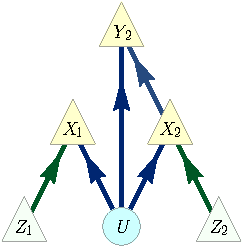
\includegraphics[scale=1]{instrumentalvariant.pdf}
    \caption{An inflation DAG which illustrates why coinciding ancestral subgraphs don't necessarily imply coinciding distributions.}
    \label{fig:ancestralsubgraphnotenough}
    \end{minipage}
\end{figure}

Equality constraint expressing coinciding distributions can be used to supplement the marginal problem, and may be of practical use for reducing the dimensionality of the problem (number of quantifiers which need to be eliminated). 

However, we are not aware of any case in which this would actually result in tighter exclusions for the distributions on the original DAG. In many cases, this can be explained by the following argument. 

Suppose two sets $\bm{X}$ and $\bm{Y}$ are inflationarily isomorphic, such that a a copy-to-copy isomorphism exists which takes $\ansubgraph[G']{\bm{X}}\leftrightarrow\ansubgraph[G']{\bm{Y}}$. If the copy-to-copy isomorphism can be extended to some copy-to-copy automorphism of the entire inflation DAG $G'$ then the constraint $P_{\bm{X}} = P_{\bm{Y}}$ is not relevant for the distributions on the original DAG. The proof is as follows.

%Suppose that there is an automorphism of the inflation DAG which takes copies of nodes to copies\footnote{Note the similarity to \emph{deck transformations} in covering space theory.} and restricts to an inflationary isomorphism $\ansubgraph[G']{\bm{X}}\sim\ansubgraph[G']{\bm{Y}}$ as above. 
If $\hat{P}$ solves the unsupplemented marginal problem, then switching the variables in $\hat{P}$ according to the automorphism still solves the unsupplemented marginal problem, since the given marginal distributions are preserved by the automorphism. Now taking the uniform mixture of this new distribution with $\hat{P}$ results in a distribution that still solves the marginal problem, and in addition satisfies the supplemented constraint $P_{\bm{X}} = P_{\bm{Y}}$.

Note that the argument does not apply if there is no copy-to-copy automorphism which restricts to $\ansubgraph[G']{\bm{X}}\sim\ansubgraph[G']{\bm{Y}}$, and it also does not apply if one uses the conditional independence relations on the inflation DAG as well, since this destroys linearity. We do not know what happens in either of these cases.





%%% T: I've commented this out since we're not concerned here with observational equivalence, and I have the feeling that it would still require a major clean-up operation. The example of 6 observationally equivalent DAGs is not very good since they are all equivalent to A <-- S --> B, which doesn't contain any latent nodes
\begin{comment}
\clearpage\section{Recognizing observationally equivalent DAGs}

%\purp{Notes to self: Comment about matching-up latent variables between causal structures, for ObsEquiv test.}

%Without loss of generality we herein consider only deterministic DAGs where all latent variables are parentless. \purp{Either prove this, or remove it. If not invoked we should discuss adding edges TO latent variables.}

One expects that an edge $A\to B$ can be added to DAG $G$ while leaving $G$ observationally invariant if the new connection does not introduce any new information about observable variables to $B$. %If the added connection does inform $B$ about some observable $C$, that's still ok so long as the new informational cannot be exploited to increase the correlation between $B$ and $C$.
We can formalize this notion in the language of sufficient statistics. To do so, however, a few background definitions are in order.

\tblue{Perfectly Predictable:} The random variable $X$ is perfectly predictable from a set of variables $\bm{Z}$, hereafter $\mblue{\bm{Z}\vDash X}$, if $X$ can be completely inferred from knowledge of $\bm{Z}$ alone. In a deterministic DAG, for example, every non-root node is perfectly predictable given its parents, ${\NamedFunction{pa}{\!X\!}\vDash X}$. Indeed, in a deterministic DAG the node $X$ is perfectly predictable from $\bm{Z}$ if $X$ is a deterministic descendant of $\bm{Z}$. Operationally, $X$ is a deterministic descendant of $Z$ if the intersection of {[the ancestors of $X$]} with {[the non-ancestors of $Z$]} is a subset of {[the descendants of $Z$]}. Happily though, perfectly predictability can be extrapolated from a causal structure with minimal effort: ${\bm{Z}\vDash X}$ if every directed path to $X$ from any root node is blocked by $\bm{Z}$. 

\tblue{Markov Blanket:} The Markov Blanket for a set of nodes $\bm{V}$, hereafter $\mblue{\NamedFunction{MB}{\!\bm{V}\!}}$, is the set of all of $\bm{V}$'s children, parents, and co-parents. The Markov Blanket is so defined because the nodes in $\bm{V}$ are conditionally independent of \emph{everything} given $\NamedFunction{MB}{\!\bm{V}\!}$. If the random variables in the Markov Blanket $\NamedFunction{MB}{\!\bm{V}\!}$ are known, then information about nodes inside $\bm{V}$ has no bearing on nodes outside the Markov Blanket and vice versa.

\tblue{Markov Partition:} \purp{New! I made this up Nov 24. Useful do you think?} A set of variables $\bm{Z}$ is a Markov Partition for a pair of random variables $X$ and $Y$, hereafter $\mblue{X\cramp{\dashv}\bm{Z}\cramp{\vdash}Y}$, if the pair are conditionally independent of eachother given \emph{any superset} of $\bm{Z}$. Operationally, this means that $X$ and $Y$ are $d$-separated by every superset of $\bm{Z}$. Equivalently, ${X\cramp{\dashv}\bm{Z}\cramp{\vdash}Y}$ if $\NamedFunction{MB}{\!\bm{V}\!}\subseteq \bm{Z}$ and $X\in \bm{V}$ while $Y\not\in \bm{V}$, or if $\NamedFunction{MB}{\!\bm{V}\!}\subseteq \bm{Z}$ and $Y\in \bm{V}$ while $X\not\in \bm{V}$. Happily though, Markov Partitions can be extrapolated from a causal structure with minimal effort: ${X\cramp{\dashv}\bm{Z}\cramp{\vdash}Y}$ if and only if $X$ and $Y$ would be in \emph{disconnected components} under the deletion of all edges initiation from $\bm{Z}$. 

\tblue{Sufficient Statistic:} A set of nodes $\bm{Z}$ is a sufficient statistic for $A$ relative to $X$, hereafter $\mblue{\bm{Z}\vdash A|X}$,
%$\bm{Z}\in\NamedFunction{SS}{\!A|X\!}$, 
if and only if all inferences about $X$ which can be made given knowledge of $A$ are also inferable \emph{without} knowing $A$ but with knowing $\bm{Z}$ instead. In other words, learning $A$ can never teach anything new about $X$ if $\bm{Z}$ is already known. If $X=A$, then the \emph{only way} $\bm{Z}$ can stand in for $A$ when making inferences about $A$ is if $A$ is perfectly predicable given $\bm{Z}$, i.e. ${\bm{Z}\vdash A|A\iff \bm{Z}\vDash A}$. If $A\neq B$ then there are four \purp{and only four?)} ways that $\bm{Z}\vdash A|X$ can be implied by a DAG: If $\bm{Z}\vDash A$, if $\bm{Z}\vDash X$, if $\NamedFunction{MB}{\!\bm{V}\!}\subseteq \bm{Z}$ and $A\in \bm{V}$ while $X\not\in \bm{V}$, or if $\NamedFunction{MB}{\!\bm{V}\!}\subseteq \bm{Z}$ and $X\in \bm{V}$ while $A\not\in \bm{V}$. \purp{Alternatively:} If $A\neq B$ then there are THREE ways that $\bm{Z}\vdash A|X$ can be implied by a DAG: If $\bm{Z}\vDash A$, if $\bm{Z}\vDash X$, and if ${A\cramp{\dashv}\bm{Z}\cramp{\vdash}X}$.

\begin{theorem}\label{theo:edgeadding}
An edge $A\to B$ can be added to $G$ without observational impact if $\NamedFunction{pa}{\!B\!}$ are a sufficient statistic for $A$ relative to all observable nodes, i.e. $\forall_{\text{observable }X}:\NamedFunction{pa}{\!B\!}\vdash A|X$.\\
In particular, the edge $A\to B$ can always be added whenever $\NamedFunction{pa}{\!B\!}\vDash A$, including, but not limited to, the instance  $\NamedFunction{pa}{\!A\!}\subseteq \NamedFunction{pa}{\!B\!}$.\\
Furthermore, the edge $\Lambda\to B$ can be also always be added whenever $\Lambda$ is latent and $\NamedFunction{MB}{\!\Lambda\!}\subseteq\NamedFunction{pa}{\!B\!}$.
\end{theorem}

We can also define an analogous condition for when an edge can be removed from a DAG without impacting it observationally.
\begin{corollary}\label{cor:edgedropping}
An edge $A\to B$ can be dropped from $G$ to form $G'$ such that $G$ and $G'$ are observationally equivalent if \sout{and only if} the edge $A\to B$ can be added (back) to $G'$ while leaving $G'$ observationally invariant per \cref{theo:edgeadding}.
\end{corollary}

On the subject of adding observationally-invariant edges, it is important to recognize when latent nodes can be introduced (or dropped) without observational impact.
\begin{theorem}\label{theo:latentadding}
A (root) latent node $\Lambda$ can be removed from $G$ without observational impact if $\Lambda$ has only one child node and no co-parents ($\Lambda$ is ``equivalent to local randomness"), or if $\Lambda$'s children are also all children of another single latent node ($\Lambda$ is ``covered-for by another latent node"). Conversely, a new root latent node $\Lambda$ can be introduced along with various outgoing edges, without observational impact, if $\Lambda$ would be equivalent to local randomness or covered-for by another latent node.
\end{theorem}

\clearpage
Naturally, two causal structures are observationally equivalent if one can be transformed into the other without observational impact, via \cref{theo:edgeadding,theo:latentadding}. Some examples of observationally equivalent scenarios, and the steps which interconvert them, are given in \cref{fig:equivalences}.
\begin{figure}[hb]
\centering
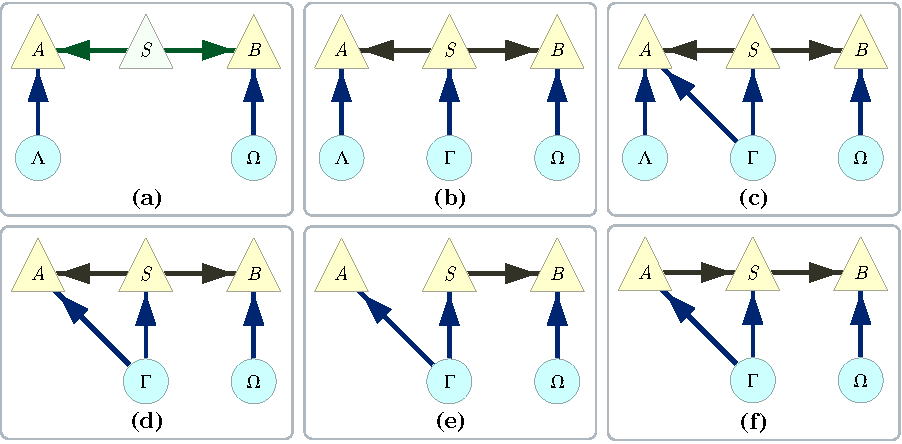
\includegraphics[width=\linewidth]{ObservationalEquivalencesExamples.pdf}
\caption{A set of observational equivalent causal structures. The reasons the changes are observational invariant are as follows: \\
(a)$\sim$(b) because $\Gamma$ is useless in (b), and as such $\Gamma$ can be dropped from (b) per \cref{theo:latentadding}.\\
(b)$\sim$(c) because $\NamedFunction{MB}{\!\Gamma\!}\subseteq\NamedFunction{pa}{\!A\!}$ in (b), and as such $\Gamma\to A$ can be added to (b) per \cref{theo:edgeadding}.\\
(c)$\sim$(d) because $\Lambda$ is redundant to $\Gamma$ in (c), and as such $\Lambda$ can be dropped from (c) per \cref{theo:latentadding}.\\
(d)$\sim$(e) because $\NamedFunction{pa}{\!S\!}\subseteq\NamedFunction{pa}{\!A\!}$ in (e), and as such $S\to A$ can be added to (e) per \cref{theo:edgeadding}.\\
(e)$\sim$(f) because $\NamedFunction{pa}{\!A\!}\subseteq\NamedFunction{pa}{\!S\!}$ in (e), and as such $A\to S$ can be added to (e) per \cref{theo:edgeadding}.
}\label{fig:equivalences}
\end{figure}

%Recall now the two steps of the transformation $\mathsf{ReduceToPCC}$. Imagine after the first step is finished, that an edge $A\to B$ remains, where $A$ is not a root node. Have directly connected all causal pathways, we know that $\NamedFunction{pa}{\!A\!}\subseteq\NamedFunction{pa}{\!B\!}$. As such, $\NamedFunction{pa}{\!B\!}\vDash A$, that is to say, $A$ is perfectly predictable given the parents of $B$. By \cref{theo:edgeadding}, therefore, if the edge $A \to B$ were not in the DAG, we would be able to add that edge without observational impact. By \cref{cor:edgedropping}, therefore, removing that edge has no observational impact. Indeed, the second step of $\mathsf{ReduceToPCC}$ leaves the post-first-step DAG observationally invariant. This allows us to quickly determine if a DAG is PCC-lossless.

%\begin{prop}\label{prop:PCClossless}
%A causal structure $G$ is PCC-lossless if every new edge in $\NamedFunction{ReduceToPCC}{\!G\!}$ relative to $G$ can be accounted for by adding edges to $G$ while leaving $G$ observationally invariant, pursuant to %\cref{theo:edgeadding,theo:latentadding}.
%\end{prop}

%%%%%%%%%%%% Enumeration via lowercase letters
\renewcommand{\labelenumi}{(\alph{enumi})}
\renewcommand{\theenumi}{(\alph{enumi})}
\renewcommand{\labelitemi}{$\circ$}
\end{comment}



\section{The Copy Lemma and Non-Shannon type Entropic Inequalities}\label{sec:NonShannon}

As it turns out, the inflation DAG technique is also useful outside of the problem of causal inference. As we argue in the following, inflation is secretly what underlies the \tblue{copy lemma} in the derivation of non-Shannon type entropic inequalities~\cite[Chapter~15]{yeung_network_2008}. The following formulation of the copy lemma is the one of Kaced~\cite{kaced_equivalence_2013}.

\begin{lemma}
	Let $A$, $B$ and $C$ be random variables with distribution $P_{ABC}$. Then there exists a fourth random variable $A'$ and joint distribution $P_{AA'BC}$ such that:
	\begin{enumerate}
		\item $P_{AB} = P_{AB'}$,
		\item $A' \perp AC \:|\: B$.
	\label{copylemma}
	\end{enumerate}
\end{lemma}

\begin{figure}[t]
\centering
\hspace{40pt}
\begin{minipage}[t]{0.23\linewidth}
\centering
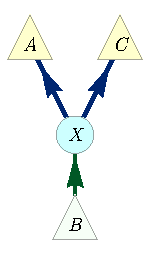
\includegraphics[scale=1]{shannonnocopy.pdf}
\caption{A causal structure that is compatible with any distribution $P_{ABC}$.}\label{fig:beforecopy}
\end{minipage}
\hfill
\begin{minipage}[t]{0.38\linewidth}
\centering
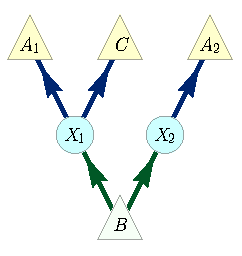
\includegraphics[scale=1]{shannonyescopy}
\caption{An inflation.}\label{fig:aftercopy}
\end{minipage}
\hspace{40pt}
\end{figure}

\begin{proof}
	Consider the original DAG of~\cref{fig:beforecopy} and the associated inflation DAG of~\cref{fig:aftercopy}. If the original distribution $P_{ABC}$ is compatible with~\cref{fig:beforecopy}, then the associated inflation model marginalizes to a distribution $P_{AA'BC}$ which has the required properties. Hence it remains to be shown that every $P_{ABC}$ is compatible with~\cref{fig:beforecopy}. But this is easy: take $\lambda$ to be any sufficient statistic for the joint variable $(A,B)$ given $C$, such as $\lambda := (A,B,C)$.
\end{proof}

While it is also not hard to write down a distribution with the desired properties explicitly~\cite[Lemma~15.8]{yeung_network_2008}, our purpose of rederiving the lemma via inflation is our hope that more sophisticated applications of the inflation technique will result in \emph{new} non-Shannon type entropic inequalities.


\section{Classifying polynomial inequalities for the Triangle scenario}
\label{sec:38ineqs}

The following polynomial inequalities for the Triangle scenario have been derived via the linear quantifier elimination method of~\cref{sec:ineqs} using the inflation DAG of~\cref{fig:Tri222}. Initially this has resulted in 64 symmetry classes of inequalities, where the symmetries are given by permuting the variables and inverting the outcomes. For the resulting 64 inequalities, numerical checks have found violations of only 38 of them: although they are all facets of the marginal polytope over the distributions on pre-injectable sets, there is no guarantee that they are also nontrivial inequalities at the level of the original DAG, and this has indeed turned out not to be the case for 26 of these symmetry classes of inequalities. Moreover, it is still likely to be the case that some of these inequalities are redundant; we have not yet checked whether for every inequality there is a distribution which violates the inequality but satisfies all others.

In the following table, the inequalities are listed in expectation-value form, where we assume the two possible outcomes of each variables to be $\{-1,+1\}$.

\purp{T: it may be better to list this as a table of coefficients, as e.g.~in \href{http://arxiv.org/abs/1101.2477}{arXiv:1101.2477}, p.14/15?}

\begin{table*}[ht]\centering\caption{List of coefficients}
\resizebox{\textwidth}{!}{
\begin{tabularx}{\linewidth}{ccccccccccccccc} 
%\begin{array}{rrrrrrrrrrrrrrrr}
  constant & \(\expec{A}\) & \(\expec{B}\) & \(\expec{C}\) & \(\expec{A B}\) & \(\expec{A C}\) & \(\expec{B C}\) & \(\expec{A B C}\) & \(\expec{A}\expec{B}\) & \(\expec{A}\expec{C}\) & \(\expec{B}\expec{C}\) & \(\expec{C}\expec{A B}\) & \(\expec{B}\expec{A C}\) &
   {\(\expec{A}\expec{B C}\)} & {\(\expec{A}\expec{B}\expec{C}\)}   \\\bottomrule
 1 & 0 & 0 & 0 & 1 & 1 & 0 & 0 & 0 & 0 & 1 & 0 & 0 & 0 & 0 \\
 2 & 0 & 0 & 0 & 0 & -2 & 0 & 0 & 0 & 0 & 0 & -1 & 0 & 0 & 1 \\
 3 & 1 & 1 & 1 & 3 & -1 & 0 & 0 & 0 & 0 & -1 & 1 & -1 & 0 & 1 \\
 3 & 1 & 1 & -1 & 3 & 1 & 0 & 0 & 0 & 0 & 1 & -1 & -1 & 0 & 1 \\
 3 & 0 & 0 & 1 & -2 & 0 & -2 & 0 & 1 & 0 & 0 & -1 & -1 & 0 & 1 \\
 3 & 0 & 1 & 0 & 1 & 0 & -2 & 0 & -1 & 1 & 0 & 1 & -1 & 0 & 1 \\
 3 & 0 & 1 & 0 & 1 & 0 & -2 & 0 & 1 & -1 & 0 & 1 & 1 & 0 & -1 \\
 3 & 1 & 1 & 1 & 2 & 2 & 2 & -1 & 1 & 1 & 1 & 1 & 1 & 1 & -1 \\
 3 & 1 & 1 & 1 & 2 & 0 & -2 & 1 & 1 & -1 & 1 & 1 & 1 & -1 & -1 \\
 4 & 0 & 0 & 2 & -2 & -2 & 0 & -1 & 2 & 0 & 2 & 1 & 1 & 1 & 0 \\
 4 & 0 & -2 & 0 & -2 & 0 & -3 & 1 & 0 & 0 & 1 & 1 & -1 & 0 & 1 \\
 4 & 0 & 0 & -2 & -2 & -2 & -3 & 1 & 2 & 0 & 1 & 1 & 1 & 0 & -1 \\
 4 & 0 & 0 & 0 & 2 & -2 & 1 & 1 & 2 & 2 & -1 & 1 & -1 & 0 & -1 \\
 4 & 0 & 0 & 0 & 2 & -2 & 1 & 1 & -2 & 2 & -1 & 1 & 1 & 0 & 1 \\
 4 & 0 & 0 & 0 & -2 & 0 & 3 & 1 & 2 & 0 & 1 & -1 & -1 & 0 & 1 \\
 4 & 0 & 0 & -2 & -2 & -2 & -2 & 1 & 2 & 0 & 0 & 1 & 1 & -1 & 0 \\
 4 & 0 & 0 & 0 & -2 & -2 & -2 & 1 & 2 & 2 & 2 & 1 & 1 & 1 & 0 \\
 5 & 1 & 1 & 1 & 3 & 1 & -4 & 0 & -2 & 0 & 1 & 1 & -1 & 0 & 1 \\
 5 & 1 & 1 & 1 & 3 & -1 & -4 & 0 & 2 & -2 & 1 & 1 & 1 & 0 & -1 \\
 5 & 1 & -1 & 1 & 1 & 2 & -2 & -2 & -2 & -1 & 1 & 1 & -2 & -2 & 0 \\
 5 & 3 & 1 & 1 & 1 & 3 & 1 & -1 & 2 & 0 & 0 & -2 & 0 & 0 & 2 \\
 5 & 1 & 1 & 1 & 1 & 2 & -2 & -1 & 0 & -1 & -1 & 2 & 1 & 1 & -2 \\
 5 & -1 & 1 & 1 & 1 & 1 & -1 & 1 & -2 & -2 & 2 & -2 & -2 & -2 & 0 \\
 5 & 1 & 1 & 1 & 2 & 1 & -1 & 1 & -1 & 0 & 2 & -1 & -2 & -2 & 1 \\
 5 & 1 & 1 & 1 & -1 & 2 & 2 & 1 & -2 & -1 & -1 & 2 & 1 & -1 & -2 \\
 6 & 0 & 0 & 0 & -3 & -4 & 0 & 0 & 1 & 2 & 2 & -1 & -2 & -2 & 1 \\
 6 & 0 & 2 & 0 & 3 & -4 & 0 & 0 & 1 & 2 & 0 & 1 & -2 & -2 & 1 \\
 6 & -2 & 2 & 0 & -3 & -5 & 0 & 0 & 1 & 1 & 0 & 1 & -1 & -2 & 2 \\
 6 & 0 & 0 & 0 & 1 & -3 & 2 & 0 & 1 & 1 & -4 & 1 & -1 & -2 & -2 \\
 6 & 0 & 0 & 2 & 0 & 3 & -5 & 0 & -2 & 1 & 1 & 2 & 1 & 1 & -2 \\
 6 & 0 & 0 & -2 & 2 & -2 & 1 & 0 & -4 & 2 & -1 & 2 & 2 & 1 & 1 \\
 6 & 0 & 0 & 0 & -3 & -2 & -2 & -2 & 1 & 0 & 4 & -1 & -2 & 0 & 1 \\
 7 & 1 & 1 & 1 & 2 & 1 & -3 & 3 & 1 & -2 & 2 & 3 & 2 & -2 & -1 \\
 8 & 0 & 0 & 0 & -4 & -2 & -2 & -3 & 4 & 2 & -2 & 1 & -1 & -3 & 2 \\
 8 & 2 & -2 & 0 & 1 & -6 & 0 & 1 & -1 & 0 & 2 & 2 & 1 & -3 & 3 \\
 8 & 2 & 0 & 0 & 6 & 1 & -2 & 1 & 0 & 1 & 2 & -1 & -2 & -3 & 3 \\
 8 & 0 & -2 & -2 & 0 & -6 & 1 & 1 & 2 & 0 & -1 & 3 & 1 & -2 & -3 \\
 8 & 0 & 0 & 2 & 2 & 1 & -6 & 1 & -2 & 1 & 0 & 3 & 2 & -1 & -3 
\end{tabularx}}
\end{table*}


\section{Other possibilities for the form of the observational data and causal hypotheses}

 A causal hypothesis is deemed \tblue{compatible} with a given distribution over observed variables if there is some causal model in the set defined by the causal hypothesis which yields this distribution, 
\begin{align}
H_{G} \quad \text{is compatible with}\quad D^{\textrm{obs}} \quad \text{iff} \quad \exists M \in H_{G} : \pdf{\SmallNamedFunction{ObservedNodes}{G}} \in D^{\textrm{obs}},
\end{align}
where $\pdf{\SmallNamedFunction{ObservedNodes}{G}}$ is fixed by the causal model $M$ through Eqs. \eqref{Markov} and \eqref{MarkovObserved}.

 
In broad strokes, the inflation DAG technique is a way of mapping a causal inference problem of this sort to a new such problem where the observational and causal inputs of the new problem are determined by the observational and causal inputs of the original problem and where compatibility between the observational and causal inputs of the original problem implies compatibility between the observational and causal inputs of the new problem.  The technique is useful because, as we show, simple witnesses of incompatibility in the new problem yield nontrivial witnesses of incompatibility in the original problem. 

The inflation DAG technique can accommodate many different forms for the observational constraints and for the causal hypothesis that appear in the original problem.  It also imposes a restriction on the forms for the observational constraints and the causal hypothesis appearing in the new problem.  It is therefore useful to pause and consider the range of possibilities for the two inputs of a causal decision problem. 

Possibilities for the form of the observational constraints include a specification of:
\begin{enumerate}
\item[O1] a joint distribution over the observed variables.
\item[O2] a confidence interval around a joint distribution over the observed variables 
\item[O3] conditional independence relations among the observed variables
\item[O3] marginals of the joint distribution for certain subsets of the observed variables
\end{enumerate}
In addition to this sort of variety, one can imagine that the statistical dependences among a set of variables may be specified not by a joint distribution but by covariance matrices or the values of entropic quantities such as mutual information.  Combinations of these possibilities are also possible.

The specification of the joint distribution, example O1, is the most restrictive form that the observational constraints can take.  Specifying a region, example O2, provides a means of expressing uncertainty about the joint distribution.  Specifying conditional independences, example O3, is the form of observational data that has been most thoroughly exploited in the development of tools for causal inference.   If one specifies marginals, as in example O4, then the causal inference problem becomes a version of the marginals problem (described in the introduction), but where the space of joint distributions from which the marginals may arise is constrained by the causal hypothesis.  

The inflation DAG technique can be applied for {\em any} of these types of observational constraints.   Nonetheless. the particular concrete applications of the inflation DAG technique that we will describe in detail in this article will consider problems where the joint distribution is specified, i.e., constraints of the form of O1.  The new causal inference problem to which this original problem is mapped by inflation, however, is one where the constraints concern marginals, i.e., they are of the form of O4.


It is also useful to exhibit some of the possibilities for the form that the causal hypothesis may take:
\begin{enumerate}
\item[H1] the full set of causal models for a particular DAG $G$
\item[H2] the full set of causal models for a particular DAG $G$ excluding those that yield conditional independence relations beyond those implies by d-separation in $G$
\item[H3] the set of causal models for a particular DAG $G$ wherein there are constraints on the manner in which particular nodes causally depend on their parents  and/or constraints on the cardinality of the set of values for particular latent variables
\item[H4] the set of causal models for a particular DAG $G$ wherein the manner in which a particular node causally depends on its parents is constrained to be equivalent, under some mapping between nodes, to the manner in which another node causally depends on its parents
\end{enumerate}
In all cases, we have left implicit the trivial constraint that the causal hypothesis must include only those DAGs for which the set of observed nodes coincides with the set of variables described in the observational data. 

The motivation for considering hypotheses of the form of H2 rather than H1 is the principle that a causal explanation should not be fine-tuned [reference]\cite{WoodSpekkens}.  If, for some observational data, a causal hypothesis of type H1 is compatible but one of type H2 is not, then it means that the conditional independences in the observational data are not a consequence of the causal structure, but rather are a consequence of the choice of parameters.  Such an explanation can be criticized on the grounds that it is fine-tuned.  Finding a causal hypothesis of type H2 that is compatible with the observational data implies that one has a non-fine-tuned explanation of that data.  The fine-tuning issue will come up in \cref{sec:classicallity} where we discuss quantum causal models. \purp{Note, not there yet...}


An example of a causal hypothesis of type H3 is that of an additive noise model: if an observed variable $Y$ has an observed variable $X$ and a latent variable $U$ as parents, then the noise is deemed additive if $Y=\alpha X + \beta U$ for some scalars $\alpha$ and $\beta$ [provide references].  Clearly, the conditional probability distributions $\pfunc{Y|XU}$ that can be achieved in such an additive noise model are a subset of the valid conditional distributions.  More general constraints on the conditional distributions have also been explored alongside constraints on the sizes of the latent variables [cite Lee-Spekkens].  
%(Note that constraints on the probability distributions over the latent variables can be understood as a kind of constraint on the causal dependences.)
%Another conceivable constraint on the parameters is a constraint on the form of the probabilities distributions over the latent variables.  

A causal hypothesis of type H4 involves a novel and unusual sort of constraint, which has not, to our knowledge been studied previously.  We include it on our list because it is the sort of causal hypothesis that appears in the new causal problem that is defined by our inflation DAG technique.  Insofar as it is usually assumed that the manner in which one node in a DAG causally depends on its parents should be completely independent of the manner in which another depends on its parents---sometimes described as the assumption of {\em autonomy} of different causal mechanisms [Pearl]---it is quite conceivable that hypotheses of type H4 have {\em no} significance besides the role that they play in the inflation DAG technique.\footnote{\color{red} We could say something here about how this suggests that one does better to think of the inflation DAG in terms of counterfactuals and twin diagrams. \color{black}.}

The inflation map takes a causal hypothesis of type H1 and maps it to a causal hypothesis of type H4.



\clearpage
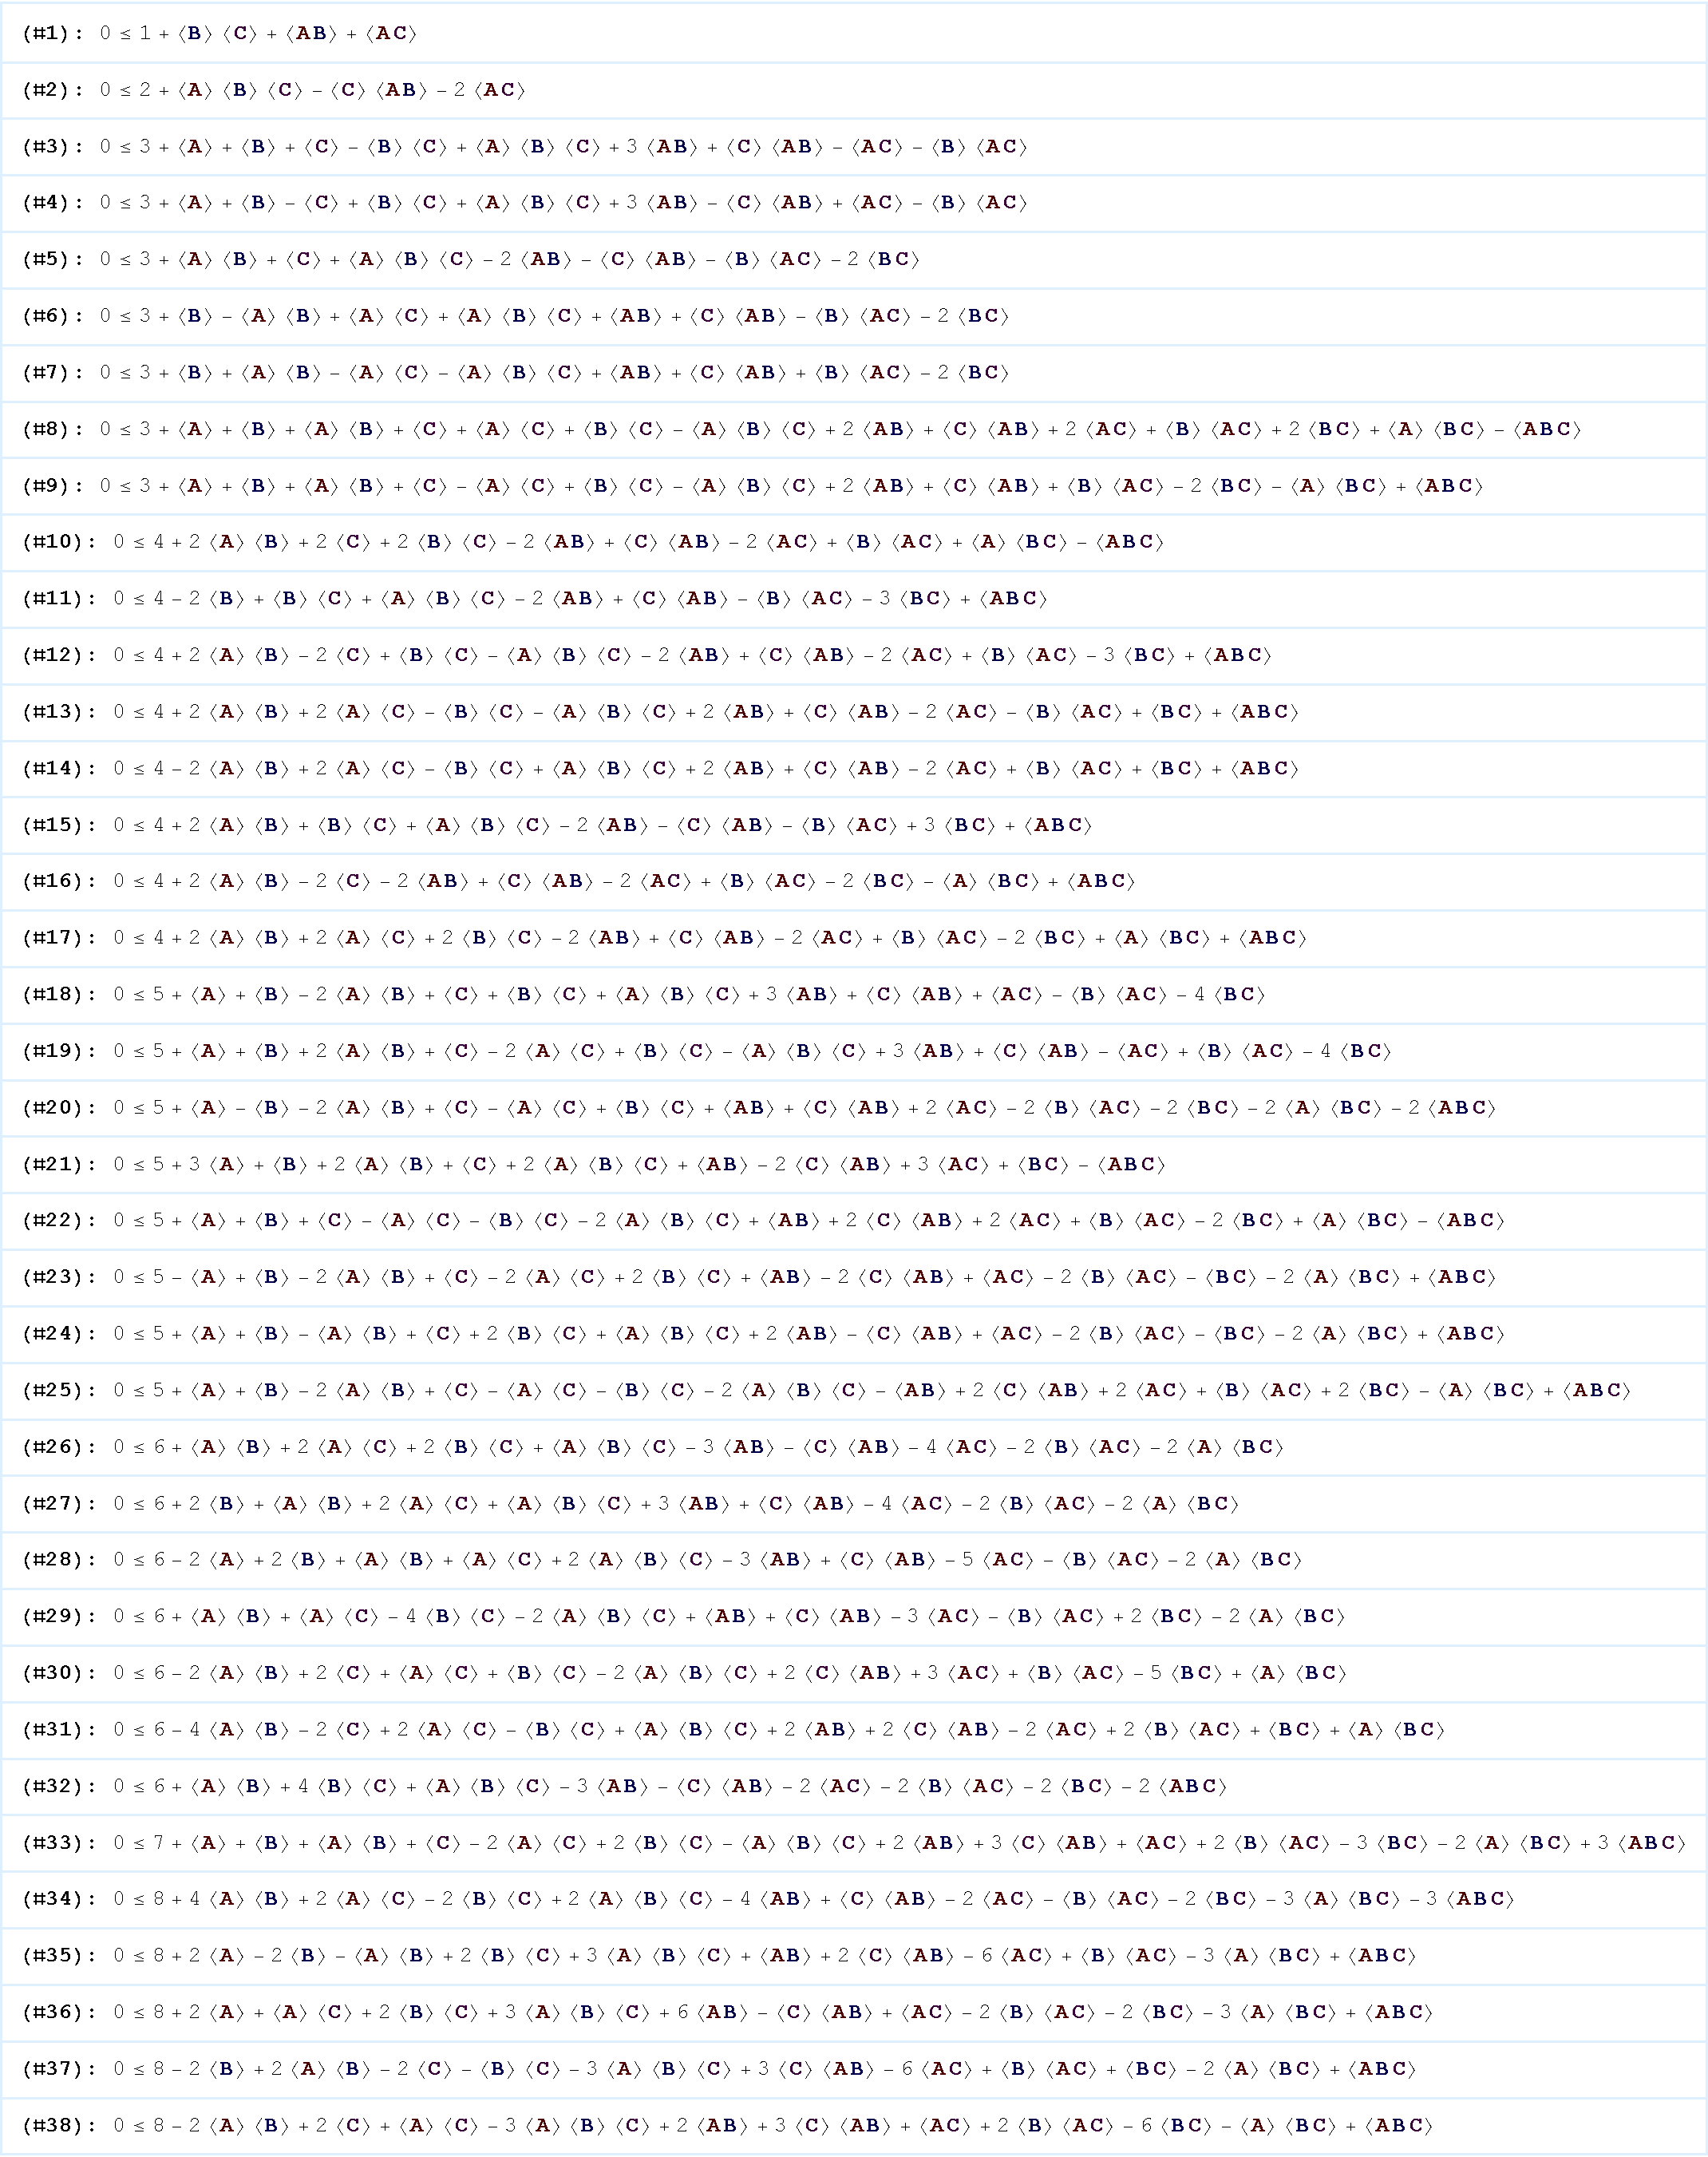
\includepdf[pages=-,scale=0.90]{nontrivlist.pdf}

%\section*{References}
%\nocite{*}
%\setlength{\bibsep}{\smallskipamount}
%\clearpage
\setlength{\bibsep}{3pt plus 3pt minus 2pt}
\bibliographystyle{apsrev4-1}
\nocite{apsrev41Control}
\bibliography{hardyinference}


\end{document}
